\documentclass[12pt,a4paper]{report}

\usepackage[margin=1in]{geometry}
\usepackage{graphicx}
\usepackage{booktabs}
\usepackage{array}
\usepackage{amsmath,amssymb}
\usepackage{siunitx}
\usepackage{caption}
\usepackage{subcaption}
\usepackage{float}
\usepackage{placeins}
\usepackage{setspace}
\usepackage{enumitem}
\usepackage{xcolor}
\usepackage{listings}
\usepackage{fancyhdr}
\usepackage[hidelinks]{hyperref}

\graphicspath{{figures/}}
\onehalfspacing
\setlength{\parindent}{1.5em}
\setlength{\parskip}{0.25em}
% Keep isolated final lines and hyphenated word fragments off the next page.
\clubpenalty=10000
\widowpenalty=10000
\displaywidowpenalty=10000
\brokenpenalty=10000
\setlength{\textfloatsep}{22pt plus 3pt minus 3pt}
\setlength{\intextsep}{18pt plus 3pt minus 3pt}
\setlength{\floatsep}{16pt plus 3pt minus 3pt}
\setcounter{secnumdepth}{3}
\setcounter{tocdepth}{2}
\sisetup{scientific-notation=true,round-mode=places,round-precision=3}
\lstset{
  language=C++,
  basicstyle=\ttfamily\footnotesize,
  columns=fullflexible,
  keepspaces=true,
  frame=single,
  rulecolor=\color{black!25},
  backgroundcolor=\color{black!3},
  showstringspaces=false,
  breaklines=true,
  xleftmargin=0.6em,
  xrightmargin=0.6em
}

\pagestyle{fancy}
\fancyhf{}
\fancyhead[LE,RO]{\thepage}
\fancyhead[LO]{Report 2}
\fancyhead[RE]{Performance of Higher-Order Methods on GPU Hardware}
\renewcommand{\headrulewidth}{0.4pt}

\begin{document}

\begin{titlepage}
\centering
\vspace*{1.0cm}
{\LARGE\bfseries Performance of Higher-Order Methods on GPU Hardware\par}
\vspace{0.45cm}
{\Large Report 2\par}
\vspace{1.6cm}

\includegraphics[width=0.19\textwidth]{University_Crest.pdf}
\vfill
{\Large Shuli Xu\par}
\vspace{0.5cm}
{\large Department of Physics\\University of Cambridge\par}
\vfill
{\large MPhil in Scientific Computing\par}
\vspace{1.1cm}
\begin{flushright}
\large Supervisor: William Bennett
\end{flushright}
\vspace{0.8cm}
{\large July 2026\par}
\end{titlepage}

\pagenumbering{roman}
% \chapter*{Abstract}
\addcontentsline{toc}{chapter}{Abstract}

Report 1 established the finite-volume Euler framework and its serial, OpenMP, and CUDA backends. Report 2 extends that framework to examine whether higher-order accuracy justifies its additional computational cost. Three schemes are compared: WENO-2 with SSPRK2 as the second-order reference, WENO-3 with SSPRK3 as a third-order method-of-lines scheme, and ADER-3 as a third-order one-step space--time method. HLLC is the official interface flux because the test set contains contact discontinuities. The validation campaign combines one- and two-dimensional smooth advection with the Sod shock tube, a two-dimensional quadrant Riemann problem, and a shock--bubble interaction. All headline values below come from the canonical HLLC results; the earlier HLL route is retained only as a matched accuracy--efficiency comparator.

Both high-order schemes recover their designed behaviour on smooth problems. On two-dimensional periodic Gaussian advection, the observed density-error orders over the finest \(800^2\)-to-\(1600^2\) refinement interval are 2.000 for WENO-2, 3.000 for WENO-3, and 3.000 for ADER-3. Complete-field comparisons also verify the numerical equivalence of the three backends: 16-thread OpenMP matches serial exactly in the stored tests, while CUDA differences are normally at or close to roundoff. The largest recorded discrepancy is the branch-sensitive shock--bubble ADER-3 energy difference of \(2.02\times10^{-7}\); the corresponding fields remain finite and positive and preserve the same resolved flow structure.

At \(600\times600\), the HLLC CUDA runs give \(L_1(\rho)\) errors of \(4.703\times10^{-7}\), \(1.726\times10^{-8}\), and \(1.681\times10^{-8}\) for WENO-2, WENO-3, and ADER-3, with runtimes of 2.08, 2.71, and 10.51 s. Thus WENO-3 and ADER-3 reduce the WENO-2 error by factors of 27.2 and 28.0, while their CUDA speedups over serial are 83.84 and 392.01; WENO-2 reaches 38.43. The discontinuous fields show that HLLC retains sharp contact-driven structure, but ADER-3 remains costly and more sensitive to its troubled-interface fallback. Phase profiling identifies reconstruction, prediction, and flux evaluation as the dominant accelerated work, with CFL reduction and state update becoming residual bottlenecks. The CUDA-only study through \(5000\times5000\) continues to reduce error without establishing a sharp saturation point. Across the tested smooth and discontinuous cases, WENO-3 with HLLC on CUDA provides the strongest overall balance of accuracy, robustness, and runtime.
 % Temporarily hidden; excluded from the body word-count check.
\tableofcontents
\clearpage

\pagenumbering{arabic}
\chapter{Introduction}
\label{chap:introduction}

 Report 1 supplies the Euler finite-volume formulation, boundary treatment, test problems, and serial/OpenMP/CUDA framework used here. Report 2 does not repeat that derivation. It compares one accepted second-order reference, WENO-2, with two new third-order routes: WENO-3 with SSPRK3 time integration and one-step ADER-3. All official Report 2 calculations use HLLC, which restores the contact wave omitted by the earlier two-wave HLL flux \cite{harten1983,toro1994,toro2009}.

The central question is whether the error reduction from WENO-3 or ADER-3 compensates for extra reconstruction, prediction, and memory traffic. The evidence is organised as follows:
\begin{enumerate}[label=\textbf{Stage \Alph*:},leftmargin=2.4cm]
    \item establish the designed convergence order on problems with exact smooth solutions.
    \item verify that serial, OpenMP, and CUDA implementations produce the same resolved flow.
    \item measure runtime, speedup, and accuracy--runtime trade-offs.
    \item compare robustness and resolved structure in discontinuous flows.
\end{enumerate}
The first two stages establish numerical correctness before performance is interpreted. The later analysis then asks which backend recovers the added cost of third-order reconstruction or prediction, and whether that cost buys a useful reduction in error. Keeping these questions separate prevents a fast but inconsistent backend, or a sharp but unstable discontinuous result, from being treated as a successful method.

\chapter{Methodology}
\label{chap:methodology}

\section{Inherited finite-volume framework}

The conserved state remains \(\mathbf U=(\rho,\rho u,\rho v,E)^T\), with the ideal-gas closure and cell-average finite-volume update defined in Report 1. Report 2 changes the interface flux, reconstruction, and temporal discretisation, but not the conservation law or data layout. In two dimensions the common spatial operator is
\begin{equation}
\mathcal L(\overline{\mathbf U}_{ij})=
-\frac{\widehat{\mathbf F}_{i+1/2,j}-\widehat{\mathbf F}_{i-1/2,j}}{\Delta x}
-\frac{\widehat{\mathbf G}_{i,j+1/2}-\widehat{\mathbf G}_{i,j-1/2}}{\Delta y}.
\label{eq:fvoperator}
\end{equation}
Here \(\overline{\mathbf U}_{ij}\) is the cell average in cell \((i,j)\),
\(\mathcal L\) is the semi-discrete finite-volume spatial operator,
\(\widehat{\mathbf F}\) and \(\widehat{\mathbf G}\) are numerical face fluxes in
the \(x\)- and \(y\)-directions, and \(\Delta x,\Delta y\) are the grid
spacings.
Reconstruction is performed separately along rows and columns, but both flux divergences enter the same update. No Strang time splitting is used.

\section{HLLC interface flux}
\label{sec:hllc}

For left and right primitive states \(\mathbf W_K=(\rho_K,u_K,v_K,p_K)\) at an \(x\)-normal face, the standard HLLC construction \cite{toro1994,toro2009} estimates the outer waves as
\begin{equation}
S_L=\min(u_L-c_L,u_R-c_R),\qquad
S_R=\max(u_L+c_L,u_R+c_R),
\end{equation}
and the contact speed is
\begin{equation}
S_M=
\frac{p_R-p_L+\rho_Lu_L(S_L-u_L)-\rho_Ru_R(S_R-u_R)}
{\rho_L(S_L-u_L)-\rho_R(S_R-u_R)}.
\label{eq:hllccontact}
\end{equation}
The subscript \(K\in\{L,R\}\) denotes the state on either side of the face,
\(c_K\) is its sound speed, \(S_L\) and \(S_R\) estimate the two outer wave
speeds, and \(S_M\) is the contact-wave speed between them.
The star-state density and energy are
\begin{equation}
\rho_K^*=\rho_K\frac{S_K-u_K}{S_K-S_M},\qquad
E_K^*=\rho_K^*\left[\frac{E_K}{\rho_K}+(S_M-u_K)
\left(S_M+\frac{p_K}{\rho_K(S_K-u_K)}\right)\right].
\end{equation}
The corresponding star pressure and conservative state are
\begin{equation}
p^*=p_K+\rho_K(S_K-u_K)(S_M-u_K),\qquad
\mathbf U_K^*=\left(\rho_K^*,\rho_K^*S_M,
\rho_K^*v_K,E_K^*\right)^T.
\label{eq:hllcstar}
\end{equation}
The superscript \(^*\) identifies a quantity in the left or right HLLC
star region, rather than in the original reconstructed state.
Thus the normal momentum is set by the contact speed, while the tangential velocity is preserved. Equations~\eqref{eq:hllccontact}--\eqref{eq:hllcstar} enforce the Rankine--Hugoniot jump relation across each outer wave and retain the linearly degenerate contact wave. This is the main distinction from the two-wave HLL flux used as the historical comparison: HLL averages over the contact-containing star region, whereas HLLC divides it into left and right star states. The flux is selected from
\begin{equation}
\widehat{\mathbf F}_{\mathrm{HLLC}}=
\begin{cases}
\mathbf F_L, & 0\le S_L,\\
\mathbf F_L+S_L(\mathbf U_L^*-\mathbf U_L), & S_L\le0\le S_M,\\
\mathbf F_R+S_R(\mathbf U_R^*-\mathbf U_R), & S_M\le0\le S_R,\\
\mathbf F_R, & S_R\le0.
\end{cases}
\label{eq:hllcflux}
\end{equation}
The \(y\)-normal form exchanges \(u\) and \(v\). A local Rusanov flux is used only when the denominator in Equation~\eqref{eq:hllccontact} is below \(10^{-14}\). This protects a degenerate interface and is not the normal flux path.

\section{WENO-3 with SSPRK3}

WENO-2 is retained unchanged as the second-order reference. Following the classical WENO construction based on candidate stencils and nonlinear smoothness weights \cite{jiang1996}, WENO-3 reconstructs a left interface value from
\begin{equation}
q_0=-\tfrac12U_{i-1}+\tfrac32U_i,\qquad
q_1=\tfrac12U_i+\tfrac12U_{i+1},
\end{equation}
where \(q_0\) and \(q_1\) are the two candidate interface values.
The quantities \(\beta_0=(U_i-U_{i-1})^2\) and
\(\beta_1=(U_{i+1}-U_i)^2\) measure the smoothness of their stencils, while
\(\tau=|\beta_0-\beta_1|\) is the WENO-Z global smoothness measure. WENO-Z
weights use
\begin{equation}
\alpha_k=d_k\left[1+\left(\frac{\tau}{\varepsilon+\beta_k}\right)^2\right],
\qquad (d_0,d_1)=(1/3,2/3),\quad \varepsilon=10^{-6},
\end{equation}
where \(d_k\) is the optimal linear weight, \(\alpha_k\) is its unnormalised
nonlinear counterpart, and \(\varepsilon\) prevents division by zero.
Normalising the \(\alpha_k\) values gives \(\omega_k\), followed by the
mapped-weight correction \cite{henrick2005,borges2008}. The mapping used in
the implementation is
\begin{equation}
g_k(\omega)=
\frac{\omega\left(d_k+d_k^2-3d_k\omega+\omega^2\right)}
{d_k^2+\omega(1-2d_k)},
\qquad
\widetilde\omega_k=\frac{g_k(\omega_k)}{\sum_j g_j(\omega_j)}.
\label{eq:mapped-weno}
\end{equation}
Here \(g_k\) is the mapping associated with stencil \(k\), and
\(\widetilde\omega_k\) is the final normalised weight used to combine the
candidate values.
The WENO-Z factor makes \(\omega_k\) approach its linear value in smooth regions, while a large smoothness indicator suppresses a stencil that crosses a discontinuity. Equation~\eqref{eq:mapped-weno} further restores the designed order near smooth critical points. Reconstruction is component-wise in \((\rho,\rho u,\rho v,E)\), with the same scalar operation applied in both coordinate directions. The right state uses the reflected stencil and weights. HLLC fluxes built from these states define \(\mathcal L\), which is advanced by SSPRK3 \cite{gottlieb2001}:
\begin{align}
\mathbf U^{(1)}&=\mathbf U^n+\Delta t\mathcal L(\mathbf U^n),\\
\mathbf U^{(2)}&=\tfrac34\mathbf U^n+\tfrac14[\mathbf U^{(1)}+\Delta t\mathcal L(\mathbf U^{(1)})],\\
\mathbf U^{n+1}&=\tfrac13\mathbf U^n+\tfrac23[\mathbf U^{(2)}+\Delta t\mathcal L(\mathbf U^{(2)})].
\end{align}
The superscript \(n\) denotes the current time level, while \((1)\) and
\((2)\) label the two intermediate Runge--Kutta stage states.

\section{One-step ADER-3}

ADER-3 replaces Runge--Kutta stages by a local space--time predictor \cite{dumbser2008}. Each cell carries the quadratic polynomial
\begin{equation}
\mathbf w_h(\xi,\eta)=\mathbf a_0+\xi\mathbf a_x+\eta\mathbf a_y
+\tfrac12\xi^2\mathbf a_{xx}+\xi\eta\mathbf a_{xy}
+\tfrac12\eta^2\mathbf a_{yy},
\end{equation}
where \(\mathbf w_h\) is the reconstructed polynomial and the
\(\mathbf a\)-coefficients represent its constant, first-derivative, and
second-derivative terms. The correction
\(\mathbf a_0=\overline{\mathbf U}_{ij}-(\mathbf a_{xx}+\mathbf a_{yy})/24\)
preserves its cell average. The predictor
\begin{equation}
\mathbf q_h=\mathbf w_h+\tau\,\partial_t\mathbf w_h
+\tfrac12\tau^2\partial_{tt}\mathbf w_h
\label{eq:aderpredictor}
\end{equation}
defines the local space--time polynomial \(\mathbf q_h\). It uses the Euler
equations to replace time derivatives by spatial flux derivatives. Two-point
Gauss quadrature in face position and time produces four HLLC evaluations per
face, averaged into one conservative update.

Here \(\xi,\eta\in[-1/2,1/2]\) are cell-local coordinates and \(\tau\in[0,\Delta t]\) is local time. The correction in \(\mathbf a_0\) is important: without it, the polynomial value at the cell centre would be mistaken for the finite-volume average and the conservative update would acquire a resolution-dependent bias. The predictor evaluates the evolving face states directly over the time step, so ADER-3 needs one flux-divergence update rather than the three complete spatial-operator evaluations used by SSPRK3. Its predictor is more expensive per face, but exposes considerably more arithmetic inside one update.

Near discontinuities, unlimited high-order prediction can form non-admissible states. An interface therefore falls back to first-order cell-average HLLC when the maximum relative jump in density, pressure, or normal velocity exceeds 0.15, or when a predicted state has non-positive density or pressure. A failed full update is retried with \(\Delta t/2\), up to eight reductions. The fallback is local, so smooth cells retain the third-order predictor.

\section{Time-step selection}

All methods use the multidimensional CFL restriction \cite{courant1967}
\begin{equation}
\Delta t=\frac{\mathrm{CFL}}
{\max(|u|+c)/\Delta x+\max(|v|+c)/\Delta y},
\label{eq:cfl}
\end{equation}
where \(c\) is the local sound speed and each maximum is taken over the active
cells in the corresponding coordinate direction. The resulting
\(\Delta t\) is the accepted time-step length and is clipped so that the last
step ends exactly at the requested final time. Smooth runs use CFL 0.4 for WENO-2/WENO-3 and 0.25 for ADER-3. Discontinuous WENO runs use 0.20. The
common ADER-3 value 0.14 is justified in Section~\ref{sec:cfl-study}.

The CFL number is method-dependent because the SSP Runge--Kutta and ADER updates have different stability limits, and the discontinuous ADER predictor also contains admissibility, fallback, and retry branches. A single CFL imposed on every method would therefore either make one scheme unreliable or force all schemes to use the most restrictive value, adding time steps that the less restrictive methods do not require. The values above were selected by stability and accuracy tests, not by timing alone: for each method and problem class, the largest tested value was retained only when the solution remained finite and positive, achieved the expected smooth-grid accuracy, and gave reproducible backend behaviour. This evaluates each scheme in a practical stable configuration while preserving a strict control within that scheme: serial, OpenMP, and CUDA always use the same CFL, grid, final time, and accepted time-step rule.

\section{Core implementation}

The C++17 code keeps the Report 1 field containers and backend interface. The new numerical work is concentrated in the WENO-3 reconstruction, SSPRK3 update, ADER-3 predictor, and HLLC flux. Serial and OpenMP call the same numerical functions. OpenMP changes loop execution only, following the shared-memory work-sharing model \cite{openmp52}. CUDA keeps the evolving field in device memory and reproduces the same method as kernels under the CUDA execution and memory model \cite{nvidia129}.

Listing~\ref{lst:weno3-core} shows the WENO-3 operation that differs from WENO-2: asymmetric third-order linear weights, WENO-Z nonlinearisation, and mapped weights. The same scalar function is applied to each conserved component in both coordinate directions.

\begin{lstlisting}[caption={Core left-state WENO-3 reconstruction used by the CPU implementation.},label={lst:weno3-core}]
const double q0 = -0.5 * uim1 + 1.5 * ui;
const double q1 =  0.5 * ui   + 0.5 * uip1;
const double beta0 = (ui - uim1) * (ui - uim1);
const double beta1 = (uip1 - ui) * (uip1 - ui);
const double tau = std::abs(beta0 - beta1);

double omega0 = nonlinear_weight_z(beta0, tau, 1.0 / 3.0);
double omega1 = nonlinear_weight_z(beta1, tau, 2.0 / 3.0);
const double alpha_sum = omega0 + omega1;
omega0 = mapped_weight(omega0 / alpha_sum, 1.0 / 3.0);
omega1 = mapped_weight(omega1 / alpha_sum, 2.0 / 3.0);
return (omega0 * q0 + omega1 * q1) / (omega0 + omega1);
\end{lstlisting}

Listing~\ref{lst:ader-core} captures the corresponding ADER-3 decision. Smooth admissible interfaces use four predicted space--time states. Troubled or non-admissible interfaces use cell-average HLLC. This branch is central to both robustness and the backend sensitivity examined later.

\begin{lstlisting}[caption={Condensed ADER-3 face-flux and local-fallback logic.},label={lst:ader-core}]
if (interface_is_troubled(left_average, right_average,
                          config.gamma, true) ||
    !polynomial_is_admissible(left_polynomial, config.gamma) ||
    !polynomial_is_admissible(right_polynomial, config.gamma)) {
    return hllc_flux_x(left_average, right_average, config.gamma);
}

Conservative2D flux_average{};
for (const double eta : face_nodes) {
    for (const double tau : time_nodes) {
        const auto left = predict_local_state(
            left_polynomial, 0.5, eta, tau,
            cell_dx, cell_dy, config.gamma);
        const auto right = predict_local_state(
            right_polynomial, -0.5, eta, tau,
            cell_dx, cell_dy, config.gamma);
        if (!is_admissible(left, config.gamma) ||
            !is_admissible(right, config.gamma))
            return hllc_flux_x(
                left_average, right_average, config.gamma);
        flux_average +=
            0.25 * hllc_flux_x(left, right, config.gamma);
    }
}
\end{lstlisting}

The submitted source repository contains the complete CPU and CUDA implementations. The excerpts above isolate the new algorithmic choices without repeating the shared storage, boundary, CSV, and command-line infrastructure already described in Report~1.

\section{Validation and backend-test design}

The convergence study uses serial smooth advection because it tests the discretisation rather than parallel execution. Density errors are evaluated against exact finite-volume cell averages using
\begin{equation}
L_1=\frac1N\sum|e_{ij}|,\qquad
L_2=\left(\frac1N\sum e_{ij}^2\right)^{1/2},\qquad
L_\infty=\max|e_{ij}|,
\end{equation}
where \(e_{ij}\) is the numerical-minus-exact cell-average density error and
\(N\) is the number of cells. The observed order between a coarse and fine
grid is
\(p_{\mathrm{obs}}=\log(\mathcal E_c/\mathcal E_f)/
\log(h_c/h_f)\), where \(\mathcal E_c,\mathcal E_f\) are the selected error
norms and \(h_c,h_f\) are the corresponding grid spacings.

The backend-consistency study fixes the grid and numerical parameters, then compares every stored primitive and conserved field from serial, 16-thread OpenMP, and CUDA. It includes periodic Gaussian advection, the four-state quadrant Riemann problem, and a planar-shock/low-density-bubble interaction. The completed Lovelace tests use double precision, two Intel Xeon Silver 4314 CPUs, and one NVIDIA A30 compiled with CUDA 12.9. Timing is not used as evidence in the validation or backend-consistency chapters.

Table~\ref{tab:evidence-matrix} separates the roles of the principal experiments. Smooth refinements test formal order. The Sod tube supplies an exact discontinuous reference. The two-dimensional discontinuous fields test contact and shock structure without an exact multidimensional solution. The backend matrix isolates implementation differences at fixed numerical parameters.

\begin{table}[H]
\centering
\small
\renewcommand{\arraystretch}{1.25}
\begin{tabular}{@{}p{0.23\textwidth}p{0.24\textwidth}p{0.18\textwidth}p{0.25\textwidth}@{}}
\toprule
Purpose & Problem & Resolution & Comparison \\
\midrule
Formal order & 1D smooth and Gaussian advection & $50$--$1600$ & Exact cell averages \\
\addlinespace[0.30em]
Formal order & 2D Gaussian advection & $25^2$--$1600^2$ & Exact cell averages \\
\addlinespace[0.30em]
Discontinuous reference & Sod shock tube, $t=0.2$ & $n=800$ & Exact Riemann solution \\
\addlinespace[0.30em]
Resolved 2D structure & Quadrant Riemann and shock--bubble, $t=0.2$ & $600^2$ & Cross-method fields and slices \\
\addlinespace[0.30em]
Backend consistency & Gaussian, quadrant and shock--bubble & $100^2$ & OpenMP/CUDA fields against serial \\
\bottomrule
\end{tabular}
\caption{Numerical evidence used before the performance analysis.}
\label{tab:evidence-matrix}
\end{table}

\chapter{Order-of-convergence validation}
\label{chap:validation}

\section{One-dimensional convergence study}

The principal order study uses \(n=50,100,200,400,800,1600\) and two smooth
periodic advection profiles. This setting isolates reconstruction and time
integration before multidimensional flux divergence is introduced. The
method-dependent CFL policy is the same as in the later experiments:
\(\mathrm{CFL}=0.40\) for WENO-2 and WENO-3 and \(\mathrm{CFL}=0.25\) for
ADER-3. Figure~\ref{fig:conv1d} gives the overall error trend, while
Tables~\ref{tab:conv1d-smooth} and~\ref{tab:conv1d-gaussian} retain every
measured local order.

\begin{figure}[H]
\centering
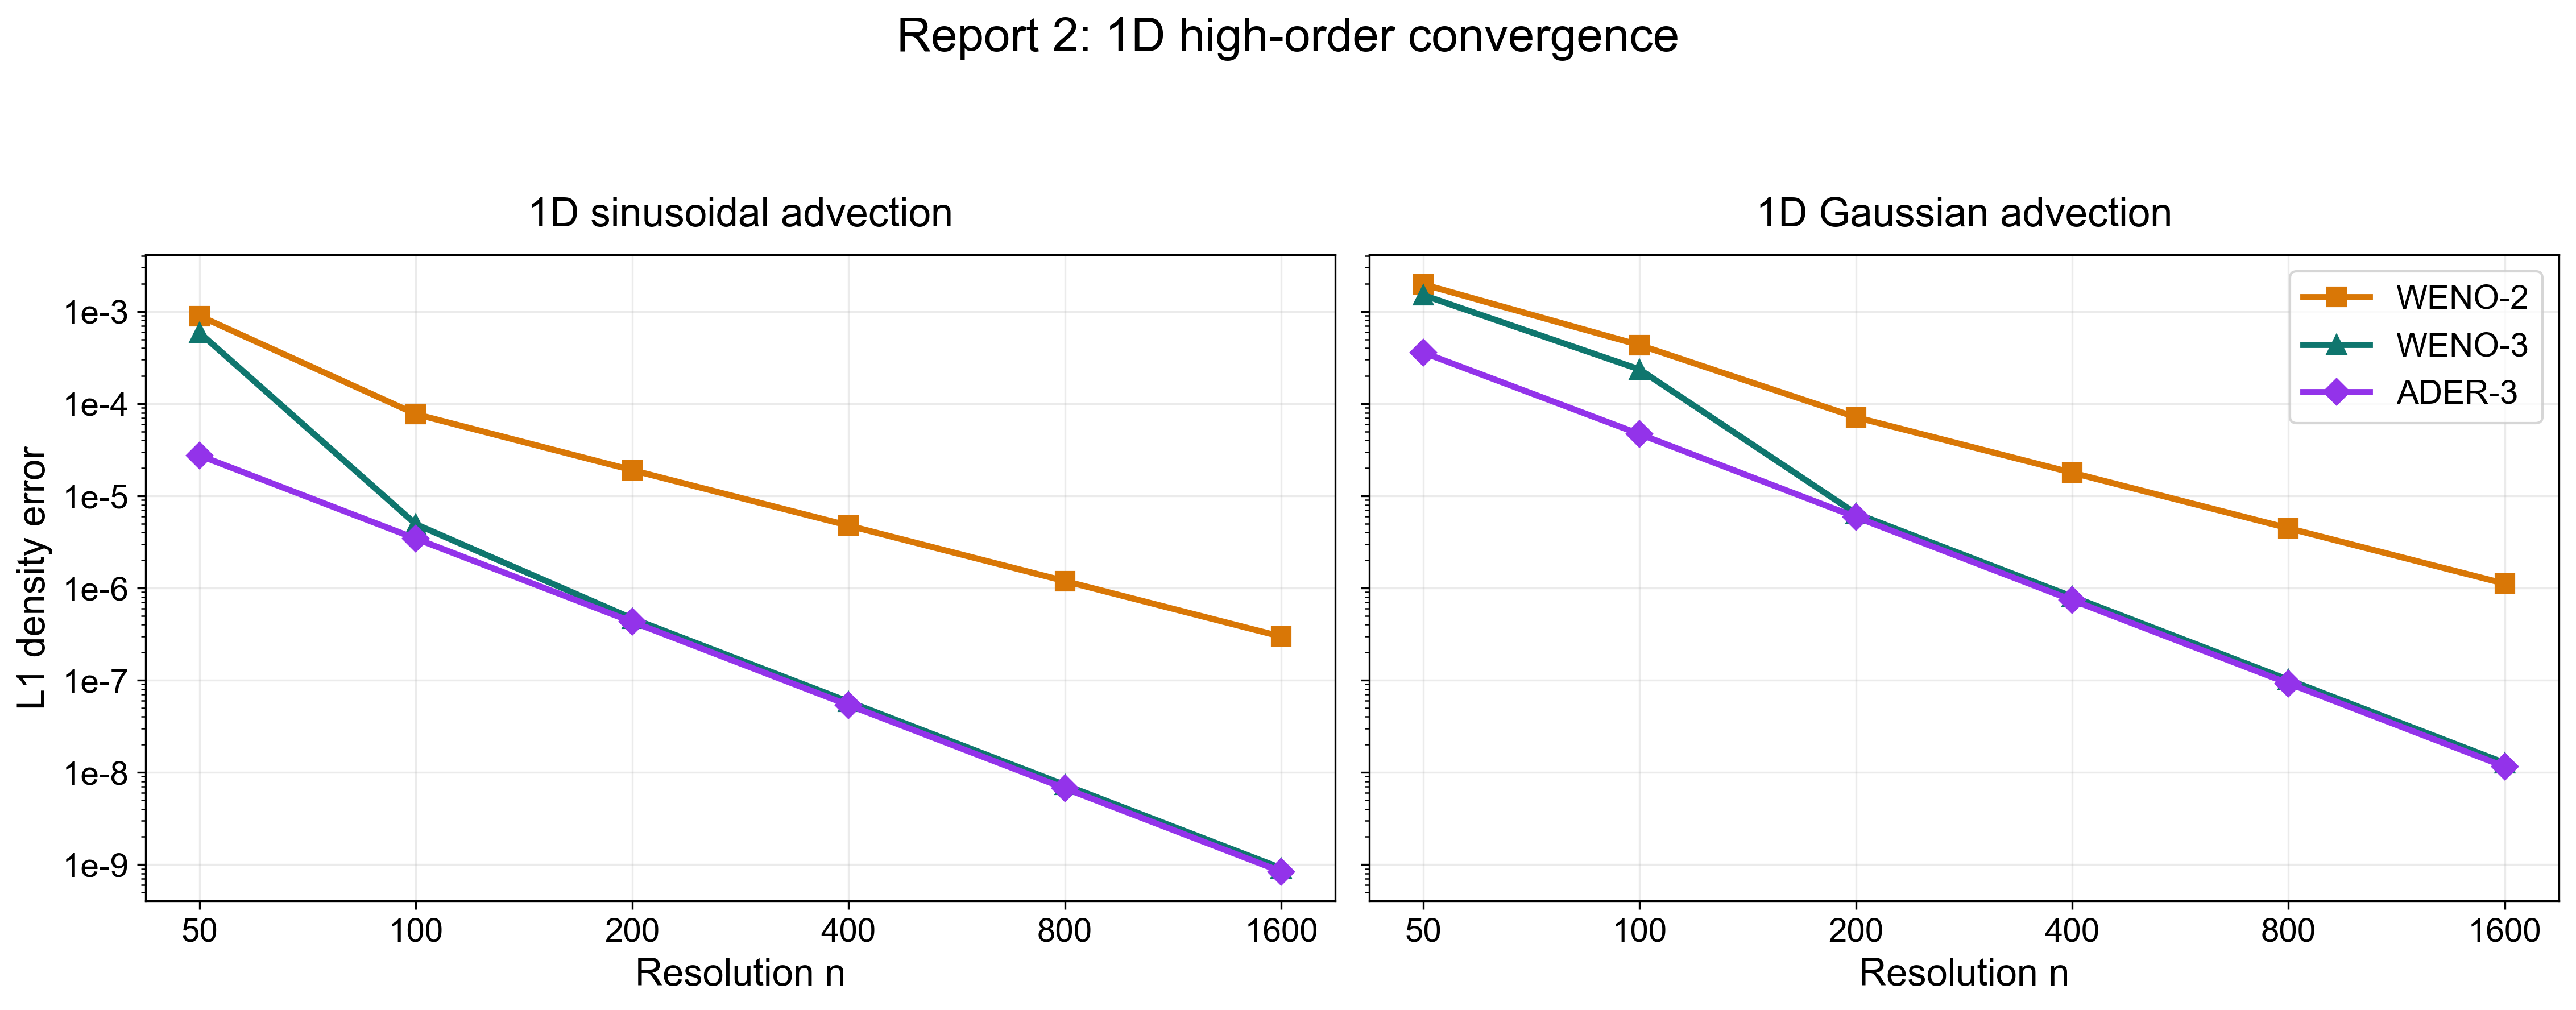
\includegraphics[width=0.97\textwidth]{convergence_1d_l1.png}
\caption{One-dimensional convergence for the smooth and Gaussian advection
profiles. Both axes are logarithmic and the plotted error is \(L_1(\rho)\).}
\label{fig:conv1d}
\end{figure}

\begin{table}[H]
\centering
\small
\setlength{\tabcolsep}{4.2pt}
\renewcommand{\arraystretch}{1.13}
\begin{tabular}{@{}r rr rr rr@{}}
\toprule
& \multicolumn{2}{c}{WENO-2} & \multicolumn{2}{c}{WENO-3}
& \multicolumn{2}{c}{ADER-3} \\
\cmidrule(lr){2-3}\cmidrule(lr){4-5}\cmidrule(l){6-7}
\(n\) & \(L_1(\rho)\) & order & \(L_1(\rho)\) & order
& \(L_1(\rho)\) & order \\
\midrule
50  & \(8.9477\times10^{-4}\) & --    & \(5.8867\times10^{-4}\) & --
    & \(2.7426\times10^{-5}\) & -- \\
100 & \(7.7022\times10^{-5}\) & 3.538 & \(4.9193\times10^{-6}\) & 6.903
    & \(3.4307\times10^{-6}\) & 2.999 \\
200 & \(1.9005\times10^{-5}\) & 2.019 & \(4.6707\times10^{-7}\) & 3.397
    & \(4.2911\times10^{-7}\) & 2.999 \\
400 & \(4.7553\times10^{-6}\) & 1.999 & \(5.8396\times10^{-8}\) & 3.000
    & \(5.3643\times10^{-8}\) & 3.000 \\
800 & \(1.1888\times10^{-6}\) & 2.000 & \(7.2996\times10^{-9}\) & 3.000
    & \(6.7055\times10^{-9}\) & 3.000 \\
1600 & \(2.9720\times10^{-7}\) & 2.000 & \(9.1246\times10^{-10}\) & 3.000
     & \(8.3818\times10^{-10}\) & 3.000 \\
\bottomrule
\end{tabular}
\caption{One-dimensional smooth-advection \(L_1(\rho)\) errors. Each order is
measured relative to the preceding grid.}
\label{tab:conv1d-smooth}
\end{table}

\begin{table}[H]
\centering
\small
\setlength{\tabcolsep}{4.2pt}
\renewcommand{\arraystretch}{1.13}
\begin{tabular}{@{}r rr rr rr@{}}
\toprule
& \multicolumn{2}{c}{WENO-2} & \multicolumn{2}{c}{WENO-3}
& \multicolumn{2}{c}{ADER-3} \\
\cmidrule(lr){2-3}\cmidrule(lr){4-5}\cmidrule(l){6-7}
\(n\) & \(L_1(\rho)\) & order & \(L_1(\rho)\) & order
& \(L_1(\rho)\) & order \\
\midrule
50  & \(1.9730\times10^{-3}\) & --    & \(1.5073\times10^{-3}\) & --
    & \(3.5844\times10^{-4}\) & -- \\
100 & \(4.3245\times10^{-4}\) & 2.190 & \(2.3519\times10^{-4}\) & 2.680
    & \(4.6774\times10^{-5}\) & 2.938 \\
200 & \(7.1327\times10^{-5}\) & 2.600 & \(6.4408\times10^{-6}\) & 5.190
    & \(5.8872\times10^{-6}\) & 2.990 \\
400 & \(1.7811\times10^{-5}\) & 2.002 & \(8.0646\times10^{-7}\) & 2.998
    & \(7.3746\times10^{-7}\) & 2.997 \\
800 & \(4.4526\times10^{-6}\) & 2.000 & \(1.0086\times10^{-7}\) & 2.999
    & \(9.2222\times10^{-8}\) & 2.999 \\
1600 & \(1.1131\times10^{-6}\) & 2.000 & \(1.2609\times10^{-8}\) & 3.000
     & \(1.1529\times10^{-8}\) & 3.000 \\
\bottomrule
\end{tabular}
\caption{One-dimensional Gaussian-advection \(L_1(\rho)\) errors. Each order
is measured relative to the preceding grid.}
\label{tab:conv1d-gaussian}
\end{table}

Both profiles give the intended asymptotic behaviour. WENO-2 settles to
second order, while WENO-3 and ADER-3 settle to third order over the finest
intervals. The isolated WENO-3 orders of 6.903 in
Table~\ref{tab:conv1d-smooth} and 5.190 in
Table~\ref{tab:conv1d-gaussian} are local pre-asymptotic transitions, not
evidence of a sixth- or fifth-order method. On these grids the nonlinear WENO
weights are moving towards their optimal smooth-flow values, while leading
spatial and temporal error components can partially cancel. Since an
observed order is computed from only two consecutive errors, that change in
the leading error coefficient temporarily produces a steep slope.

More generally, local orders on the coarsest meshes need not equal the formal
order. A smooth profile is then represented by relatively few cells, the WENO
smoothness weights have not yet reached their optimal linear limits, and
spatial, temporal, phase, and amplitude errors can have comparable sizes.
Refinement suppresses the higher error terms until a single leading term
\(C h^p\) dominates, where \(h\) is the grid spacing, \(p\) is the formal
order, and \(C\) is a grid-independent leading-error coefficient.
Consequently, the order claim is based on the stable
fine-grid sequence and its normalised-error plateau, rather than on an average
that would mix pre-asymptotic and asymptotic intervals.

The subsequent data distinguish this effect from a failed convergence test.
For smooth advection, \(L_1(\rho)n^3\) is 3.737 throughout
\(n=200,400,800,1600\). For Gaussian advection it is 51.53, 51.61, 51.64,
and 51.65.
Multiplication by \(n^3\) removes the expected third-order grid dependence,
so a nearly constant value is the estimated leading coefficient rather than
another error norm. These nearly constant normalised errors demonstrate a stable \(n^{-3}\)
asymptote. The anomalous local slopes are therefore retained as part of the
measured transition, but the formal conclusion is taken from the stable fine
grid sequence rather than from a single coarse-to-fine interval.

\section{Two-dimensional confirmation}

The two-dimensional cell-averaged Gaussian benchmark provides a concise
multidimensional check at \(t=0.1\). Rather than repeating the full 1D
refinement discussion, Figure~\ref{fig:conv2d} shows the complete refinement
sequence. The 1D results show that formal order is most reliably measured once
the grid is sufficiently fine, so Table~\ref{tab:conv2d} concentrates on the
three intervals from \(200^2\) to \(1600^2\). The reference values are exact
finite-volume cell averages, and the official smooth CFL values are used.

\begin{figure}[H]
\centering
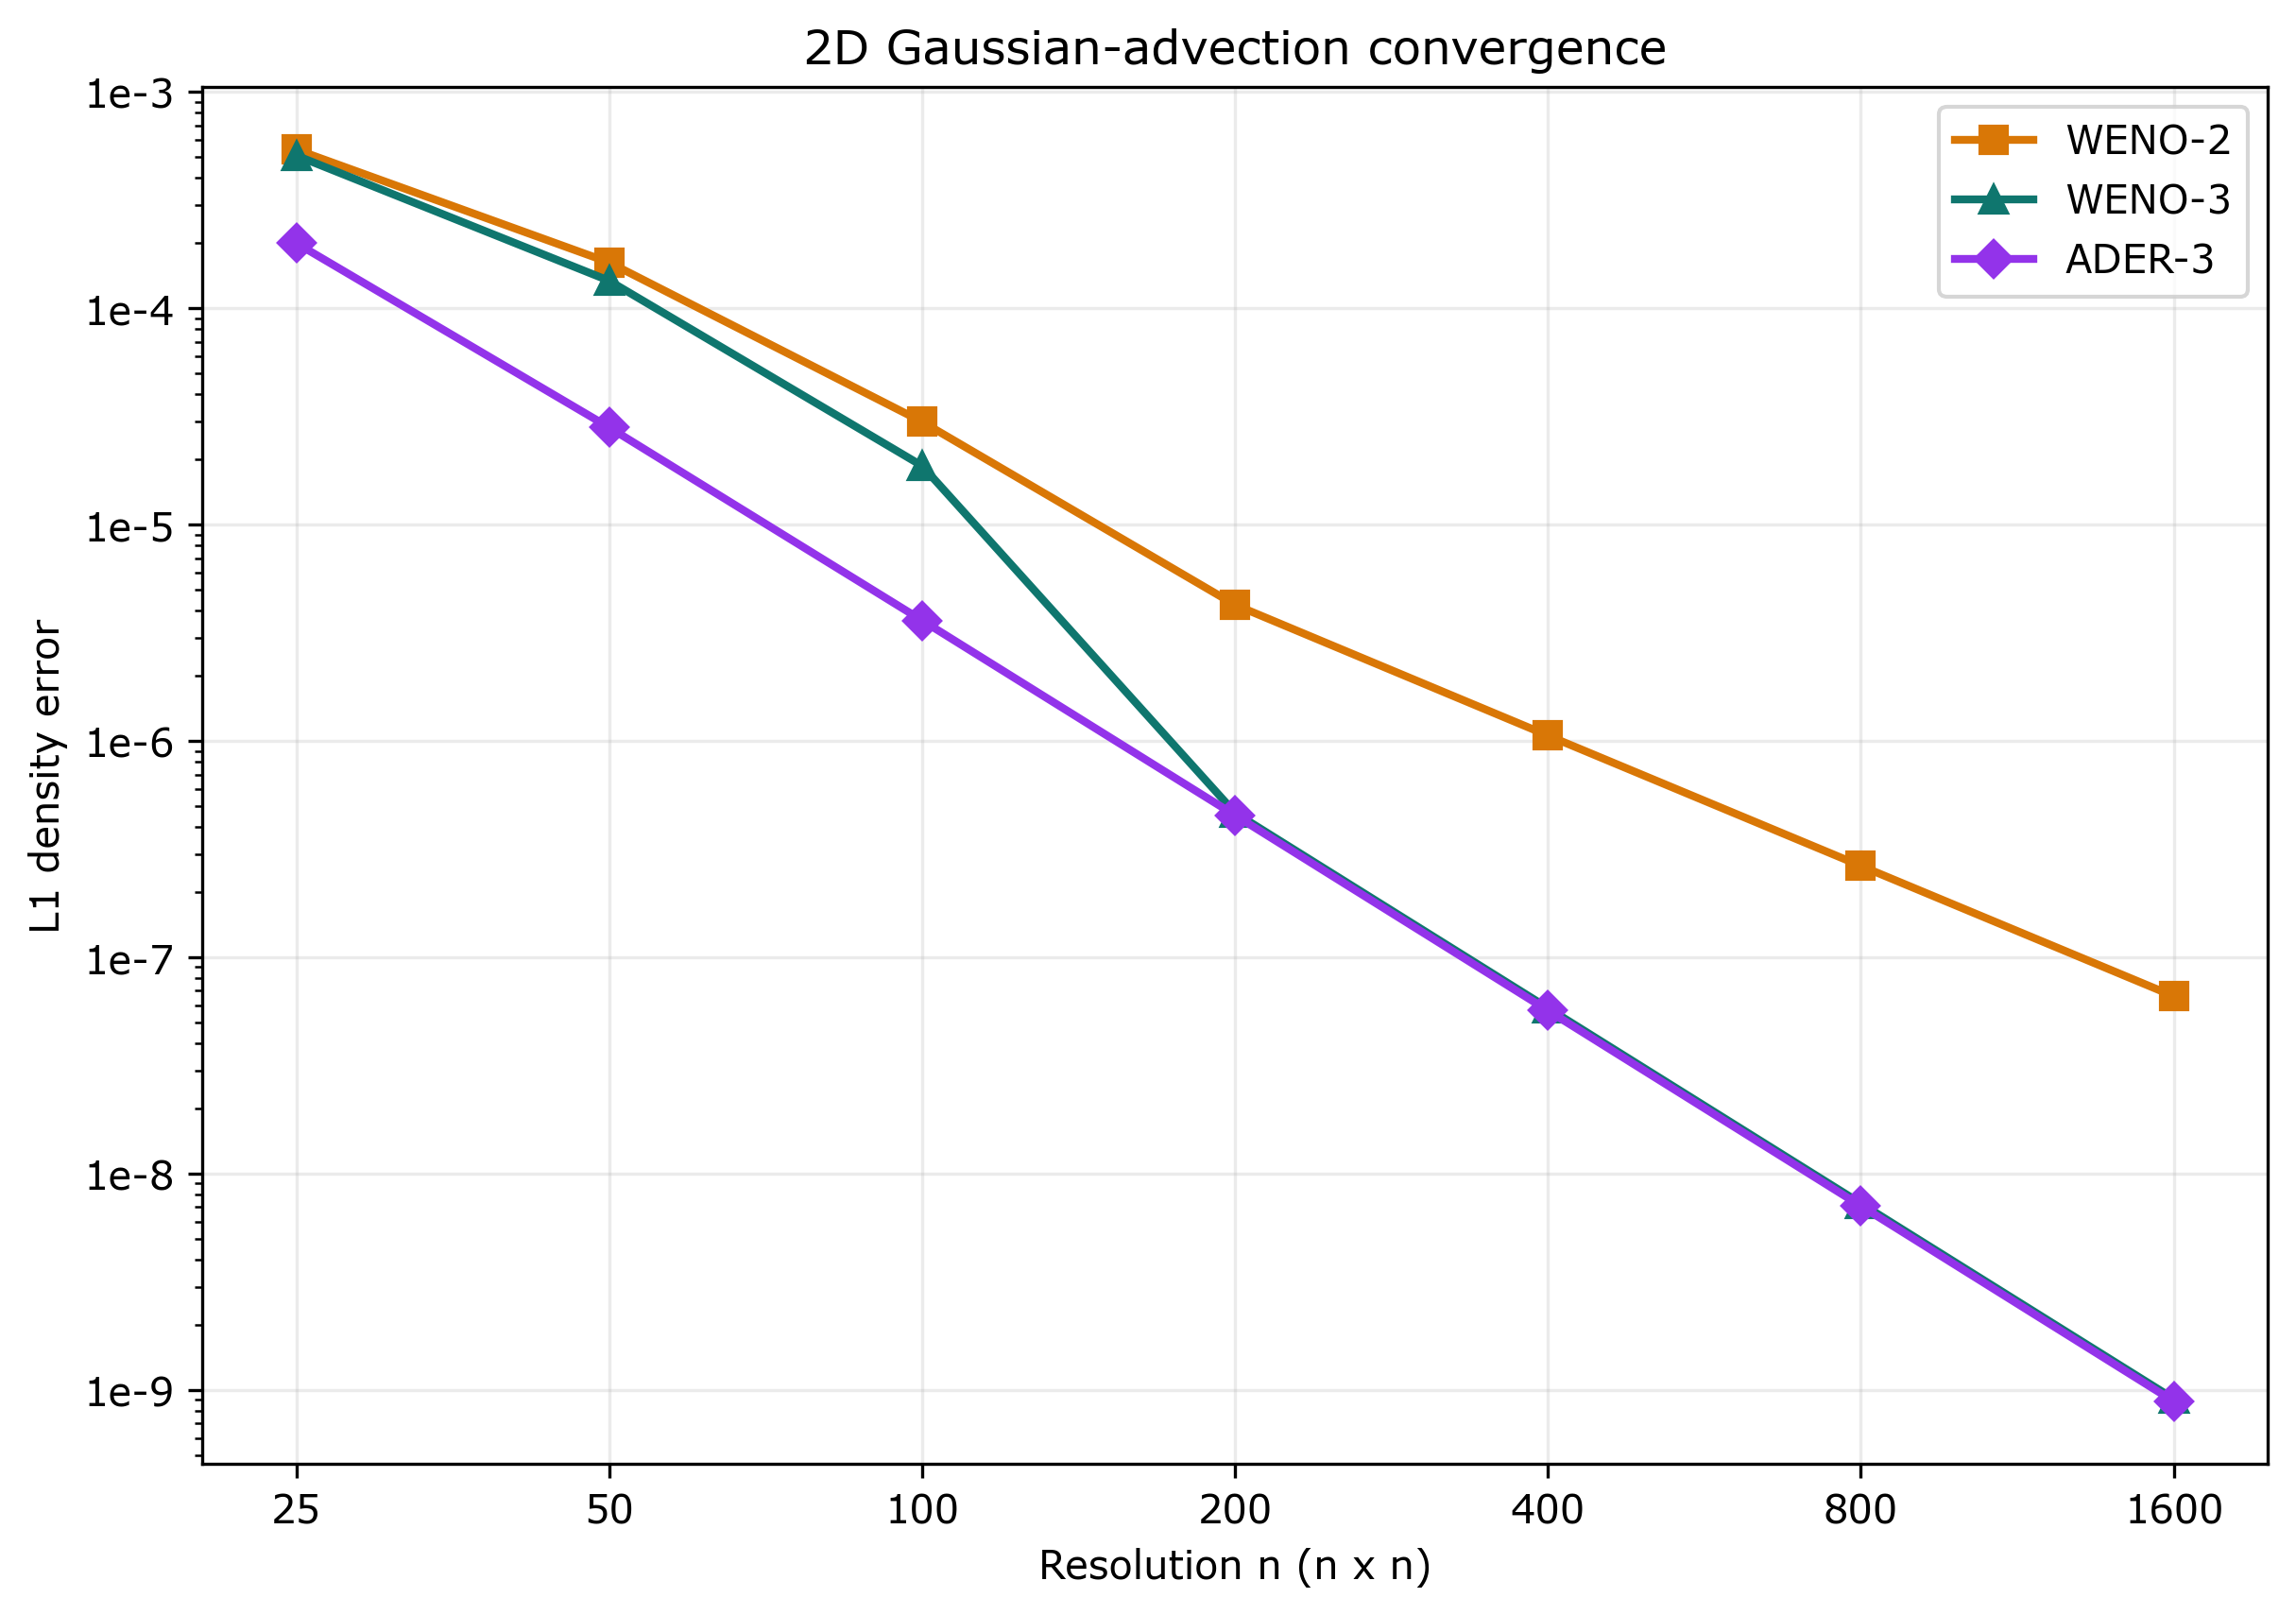
\includegraphics[width=0.86\textwidth]{convergence_2d_l1.png}
\caption{Two-dimensional Gaussian-advection \(L_1(\rho)\) convergence over
the complete \(25^2\)-to-\(1600^2\) refinement sequence.}
\label{fig:conv2d}
\end{figure}

All three errors decrease monotonically. WENO-2 settles onto its second-order
trend, while WENO-3 and ADER-3 become parallel on the fine grids and follow a
third-order trend. The unusually steep WENO-3 segment between \(100^2\) and
\(200^2\) is the same pre-asymptotic cancellation effect discussed above. It
is not interpreted as fifth-order convergence. The final three intervals
therefore provide the clean quantitative comparison.

\begin{table}[H]
\centering
\renewcommand{\arraystretch}{1.15}
\begin{tabular}{lrrrr}
\toprule
Method & \(p_{200\to400}\) & \(p_{400\to800}\) & \(p_{800\to1600}\)
& \(L_1(\rho)\) at \(1600^2\) \\
\midrule
WENO-2 & 2.007 & 2.001 & 2.000 & \(6.6102\times10^{-8}\) \\
WENO-3 & 2.998 & 3.000 & 3.000 & \(9.1051\times10^{-10}\) \\
ADER-3 & 2.998 & 3.000 & 3.000 & \(8.8664\times10^{-10}\) \\
\bottomrule
\end{tabular}
\caption{Fine-grid two-dimensional Gaussian-advection \(L_1(\rho)\) orders.
Each order is measured relative to the preceding grid.}
\label{tab:conv2d}
\end{table}

Across all three fine-grid intervals, the multidimensional result independently
recovers second order for WENO-2 and third order for WENO-3 and ADER-3. The
stability of these consecutive slopes confirms that the methods have entered
their asymptotic regimes, rather than merely producing one favourable order
estimate. On the \(1600^2\) grid, the two
third-order methods reduce the \(L_1\) density error by factors of 72.6 and
74.6 relative to WENO-2, and their errors differ by only 2.7 percent. This
fine-grid confirmation is sufficient to show that multidimensional flux
divergence and the ADER space--time construction preserve the orders already
established by the more complete 1D studies.

\chapter{Backend consistency and physical verification}
\label{chap:backend-consistency}

This chapter begins the computational-results part of the report. Its purpose is to establish
that later runtime comparisons refer to physically credible solutions and to the same
resolved numerical solution on each backend. A backend-difference map is meaningful only
when viewed beside the physical field from which it was obtained. Each two-dimensional
case is therefore followed from its resolved evolution and final field to a method-comparison
slice and, finally, the much smaller backend discrepancy. Exact one-dimensional references
and positivity checks complete the verification.

\section{Comparison procedure}

The backend study uses the official HLLC implementations of WENO-2, WENO-3
and ADER-3.  Two resolutions serve different purposes in this chapter.  The
cell-by-cell backend-consistency matrix uses a \(100\times100\) grid, which is
sufficient to expose implementation differences while keeping the full
serial--OpenMP--CUDA matrix manageable.  The resolved physical-field figures
use \(600\times600\) grids so that smooth profiles, contacts and shock-driven
structures are displayed without coarse-grid visualisation error.

For each problem--method pair in the \(100\times100\) consistency matrix, the
complete exported fields from serial, 16-thread OpenMP and CUDA are compared
cell by cell, with serial as the reference.  Maximum absolute backend
differences are evaluated separately for density \(\rho\), velocity components
\(u\) and \(v\), pressure \(p\), and total-energy density \(E\). The largest of
these five discrepancies is reported below.  These are backend-consistency
differences, not errors relative to an exact solution.  The same check verifies
that every exported value is finite and records the minimum density and
pressure for the admissibility assessment.

The CFL values follow the stable method-specific policy established in
Chapter~\ref{chap:methodology}.  Smooth WENO-2 and WENO-3 use CFL \(0.40\),
whereas smooth ADER-3 uses \(0.25\).  For both discontinuous problems, the
WENO methods use CFL \(0.20\) and ADER-3 uses \(0.14\).  Within each
problem--method comparison, all three backends use the same grid, CFL,
final time, initial and boundary conditions, and time-step formula. Only
the execution backend changes.

\section{One-dimensional physical verification}

\subsection*{Continuous advection}

The one-dimensional evidence begins with periodic sinusoidal and Gaussian advection.
These two profiles test complementary aspects of smooth transport: the sinusoid exposes
phase and amplitude errors across the full domain, whereas the compact Gaussian exposes
peak damping and broadening. Figure~\ref{fig:continuous-1d-fields} compares all three
methods with exact cell-average references at \(n=800\).

\begin{figure}[!htbp]
\centering
\begin{subfigure}[t]{0.49\textwidth}
\centering
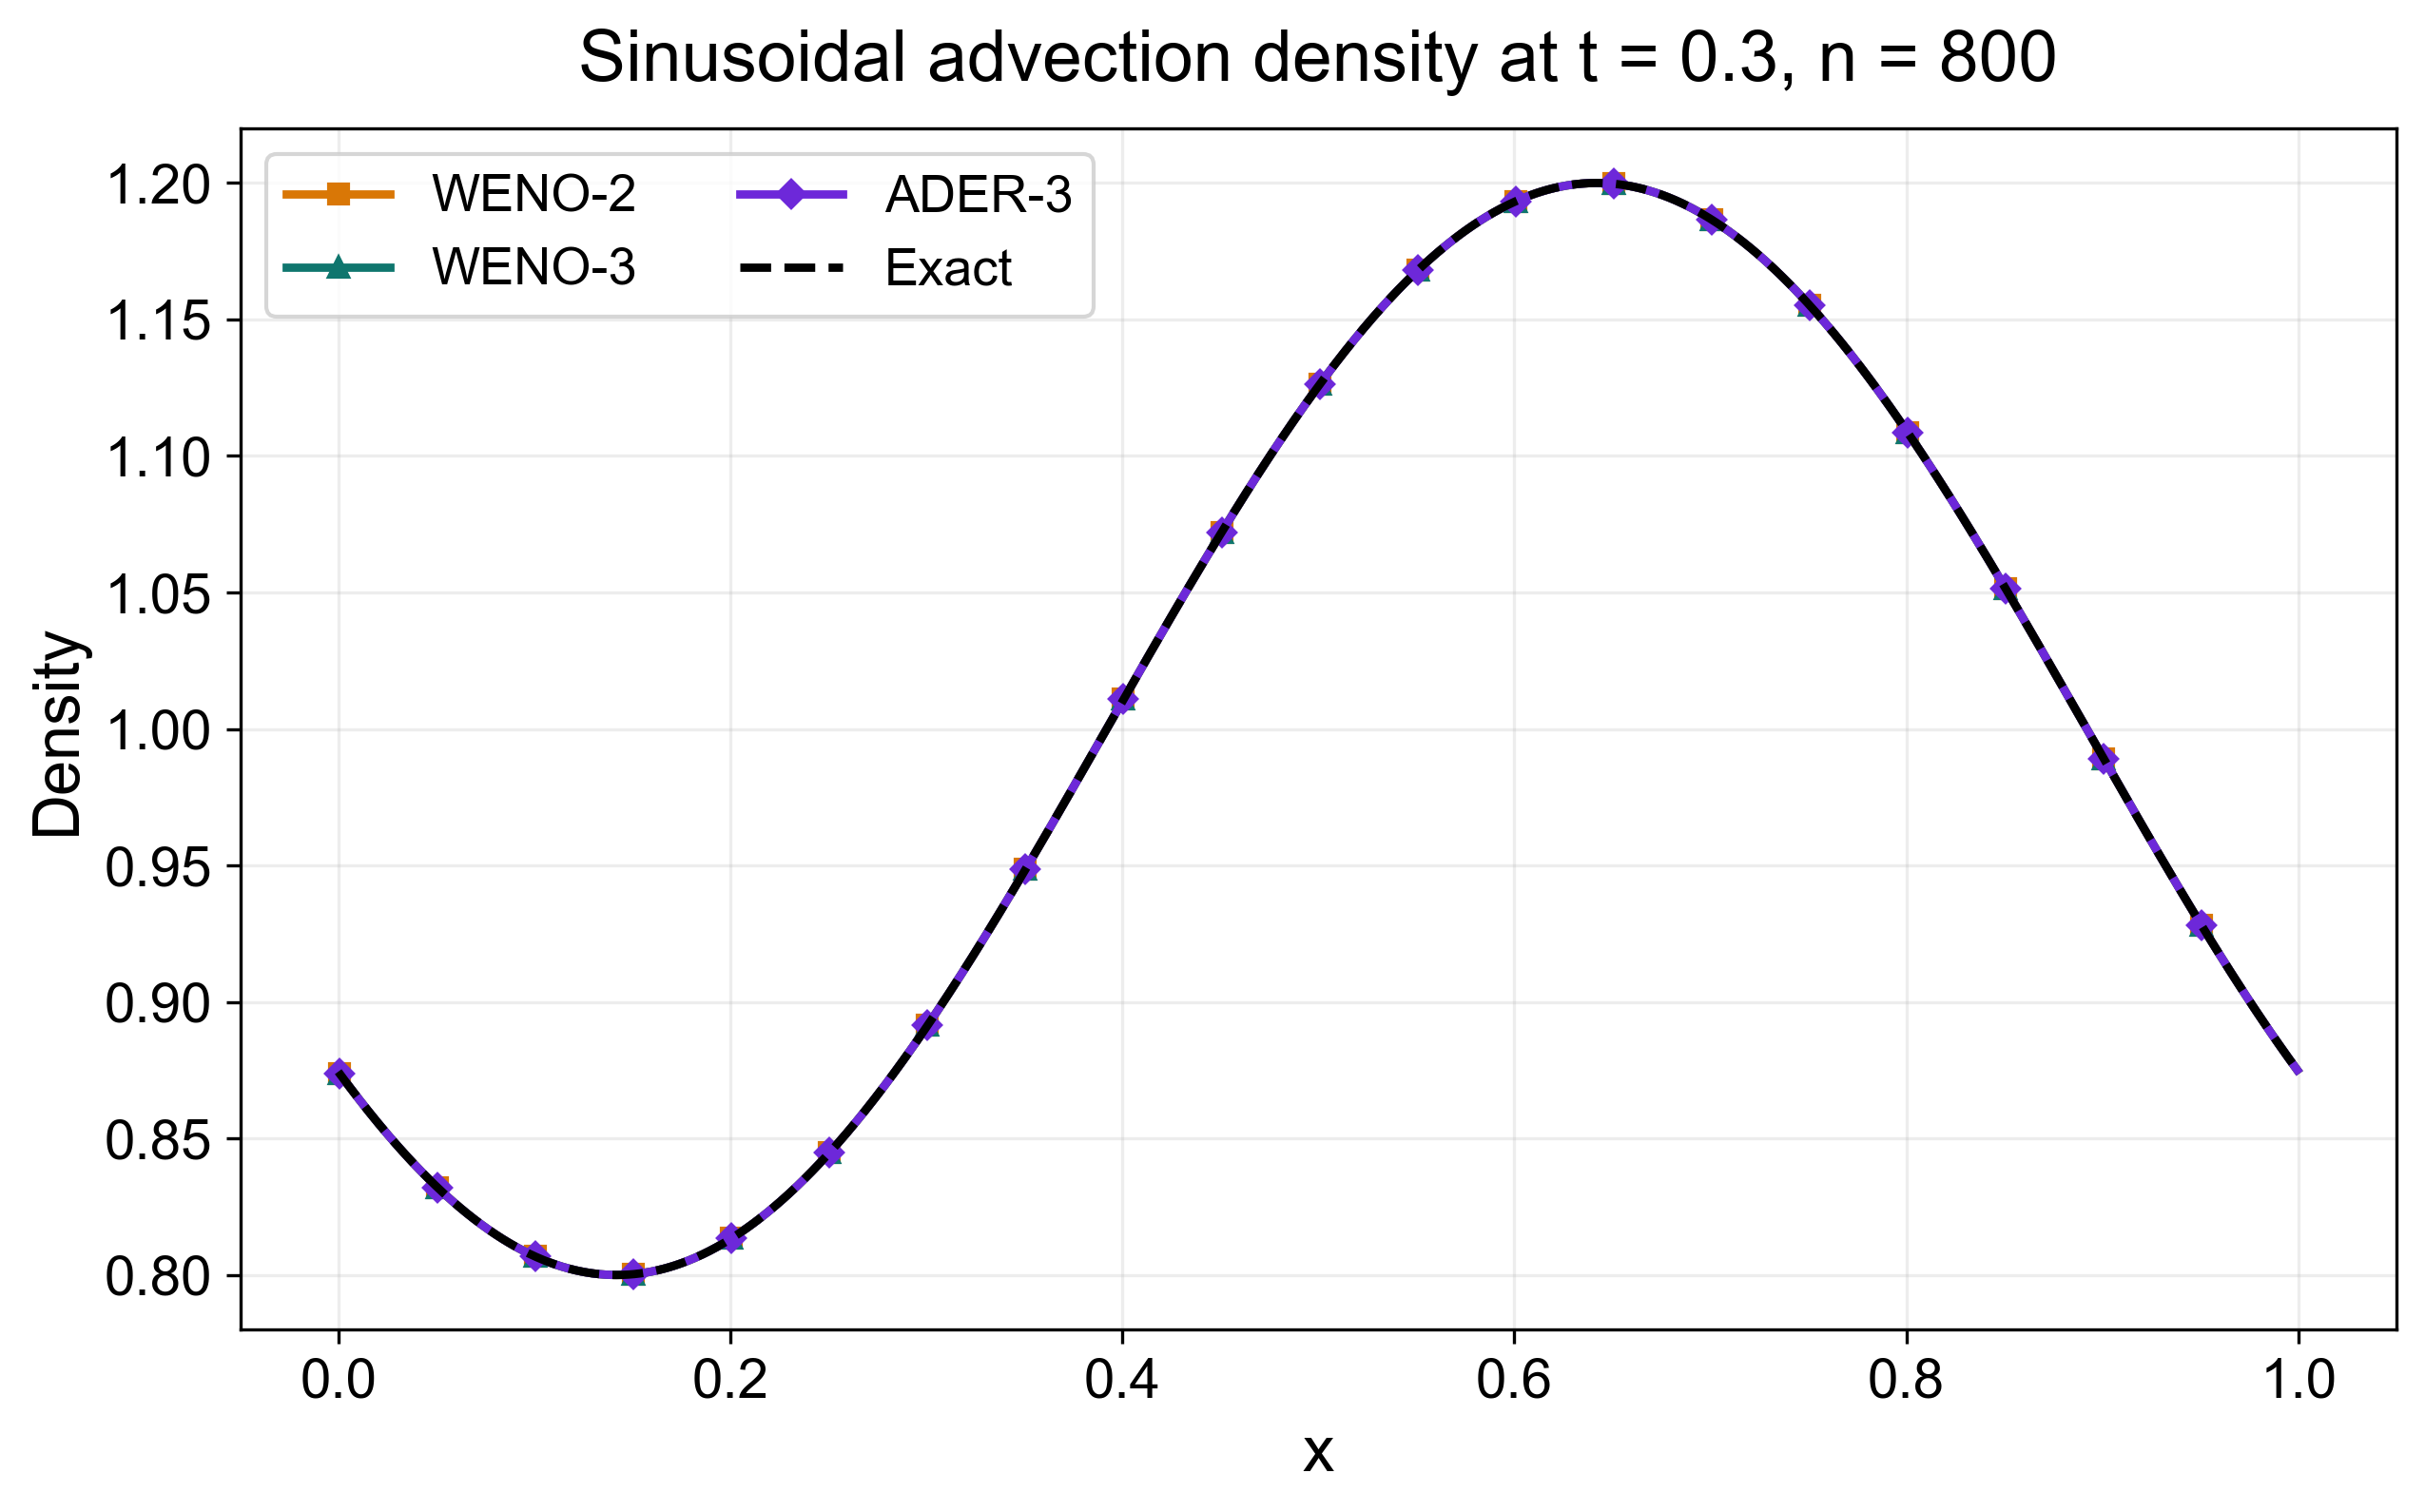
\includegraphics[width=\linewidth]{smooth_advection_hllc_n800.png}
\caption{Sinusoidal advection.}
\end{subfigure}\hfill
\begin{subfigure}[t]{0.49\textwidth}
\centering
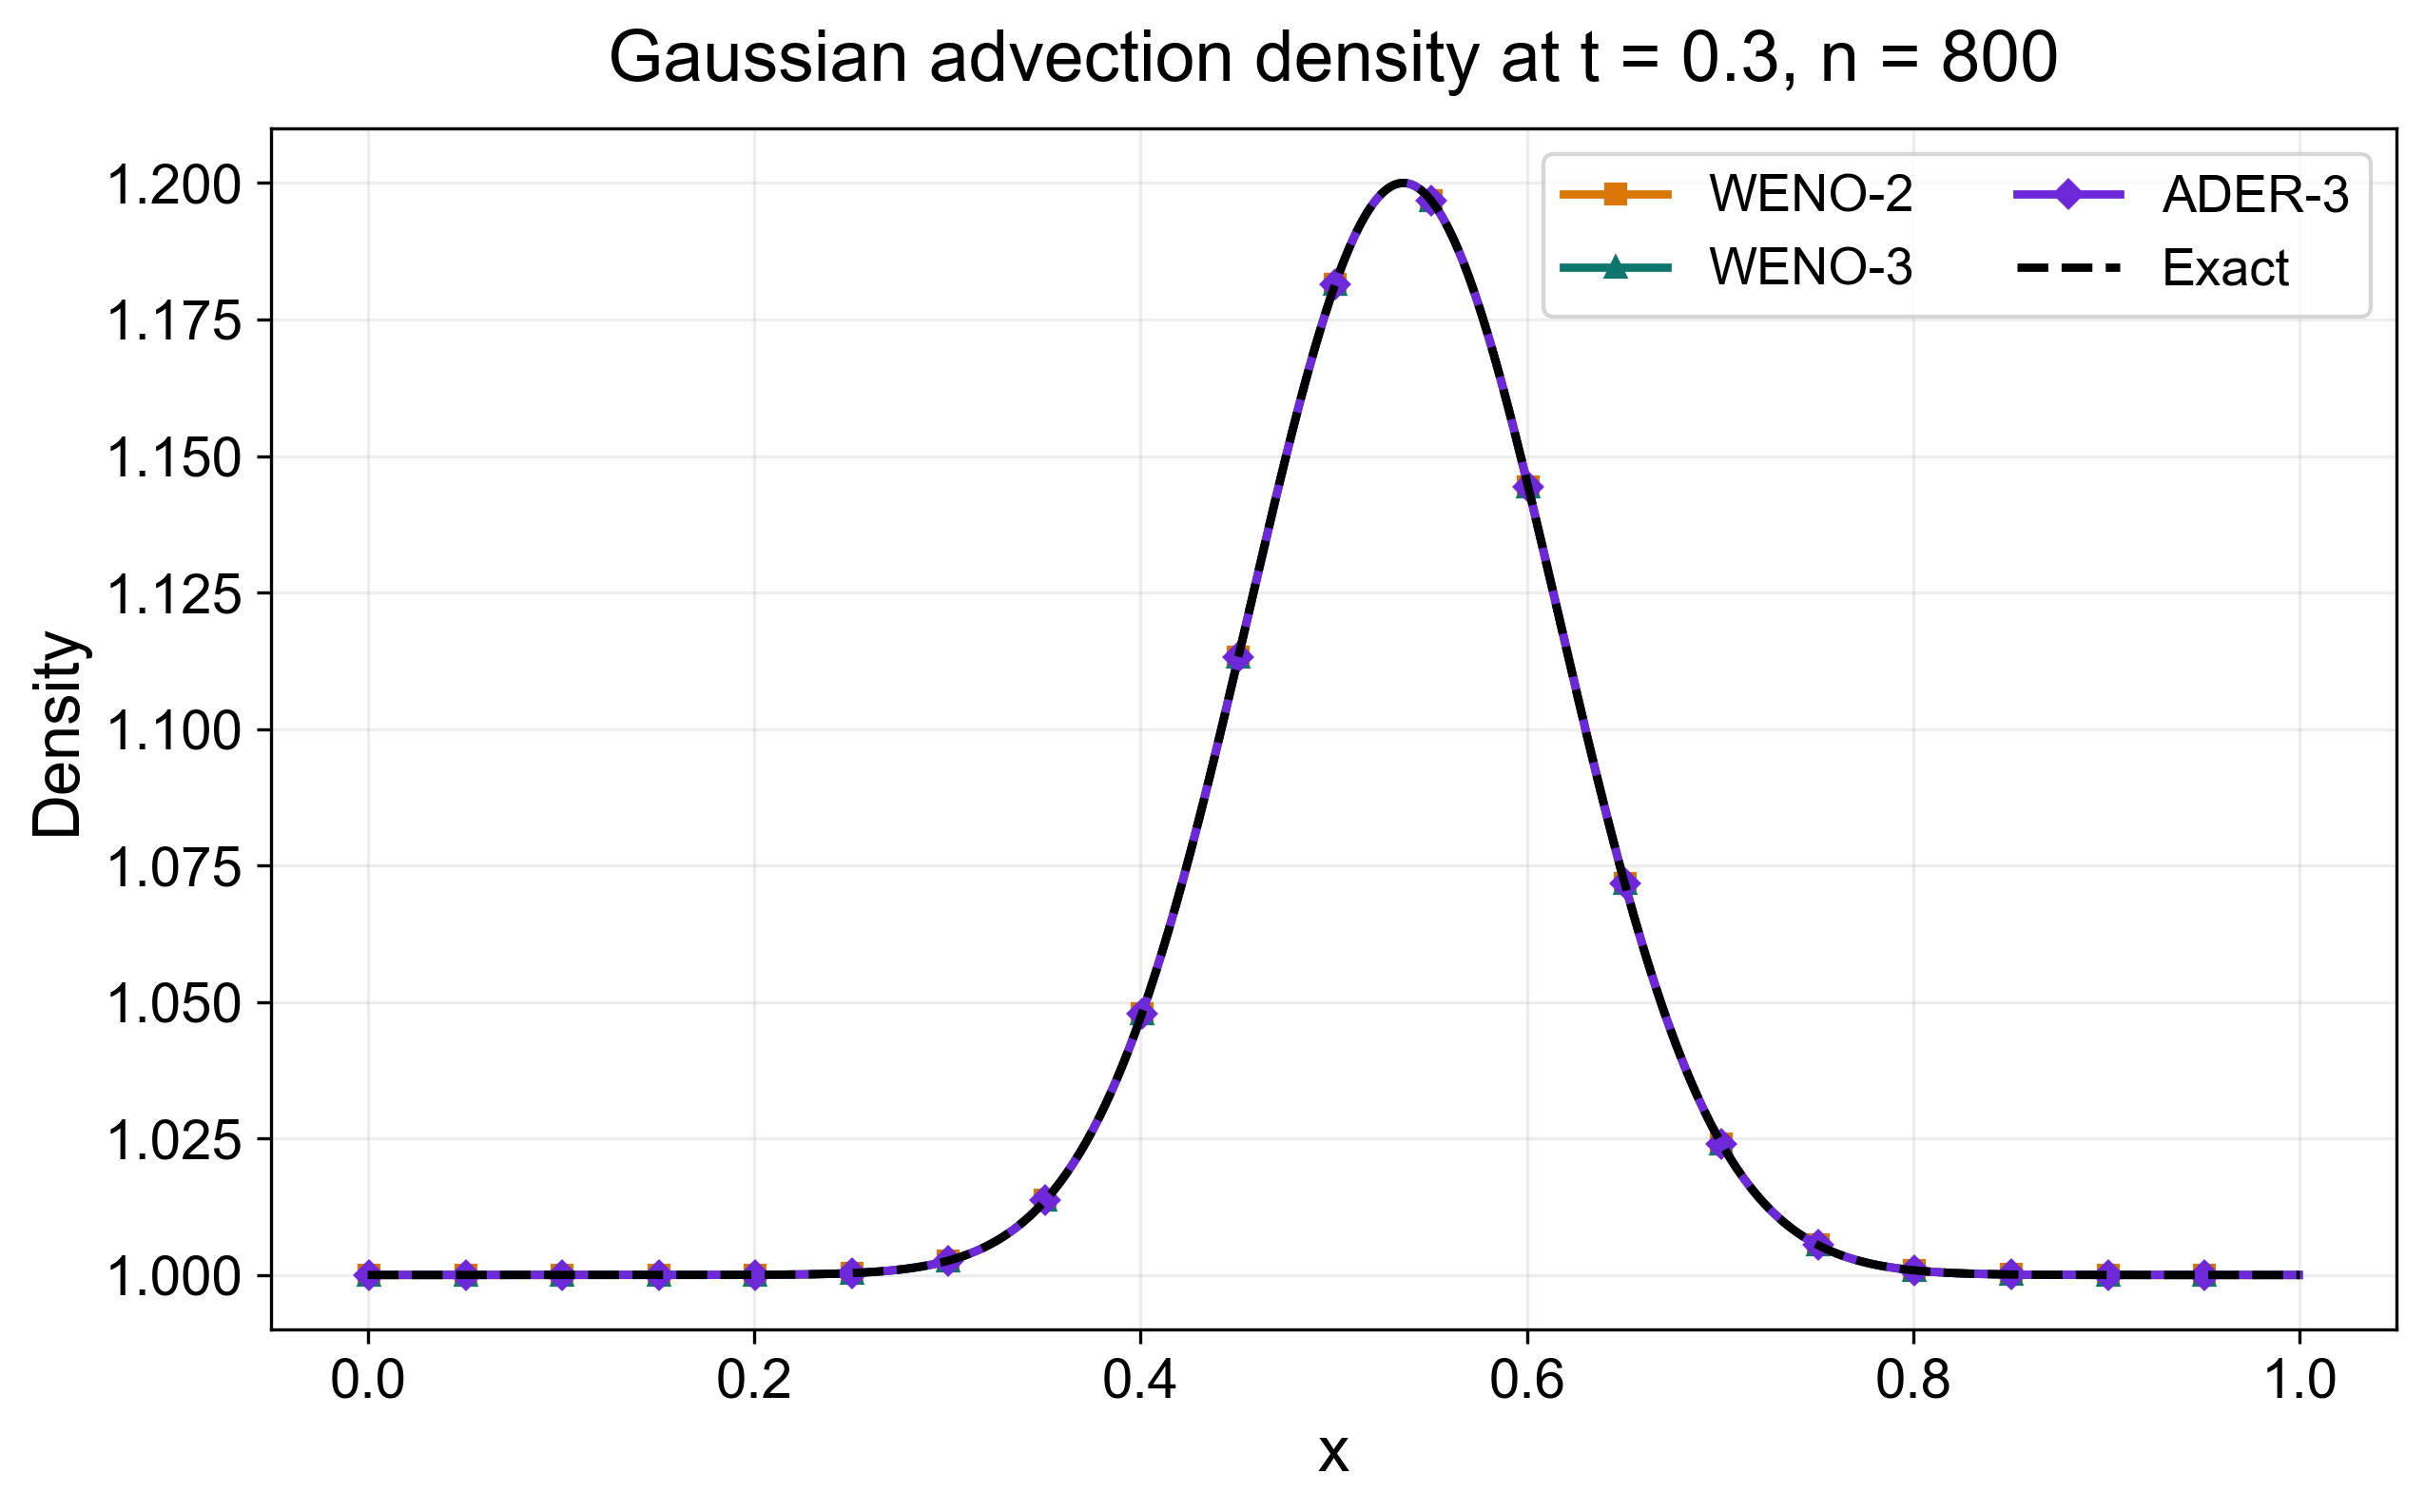
\includegraphics[width=\linewidth]{gaussian_advection_1d_hllc_n800.png}
\caption{Gaussian advection.}
\end{subfigure}
\caption{One-dimensional continuous HLLC validation at \(t=0.3\) and \(n=800\).
The dashed curves are exact cell-average solutions. Numerical markers are thinned for
readability.}
\label{fig:continuous-1d-fields}
\end{figure}

The numerical curves are visually coincident with the exact profiles: the sinusoid has
no resolved phase displacement and the Gaussian peak has no visible shift or flattening.
The corresponding convergence study in Chapter~\ref{chap:validation}, specifically
Figure~\ref{fig:conv1d} and Tables~\ref{tab:conv1d-smooth}--\ref{tab:conv1d-gaussian},
quantifies the \(L_1(\rho)\) errors that are too small to distinguish in
Figure~\ref{fig:continuous-1d-fields}. It shows WENO-2 approaching second order and
WENO-3 and ADER-3 approaching third order through \(n=1600\).

\subsection*{Discontinuous reference}

The Sod shock tube complements that continuous evidence with an exact discontinuous
reference. Its Riemann solution contains a rarefaction, contact discontinuity and shock,
so it tests whether the methods preserve the correct wave ordering and locations.
Figure~\ref{fig:sod-hllc} compares all three HLLC methods with that reference at
\(n=800\).

\begin{figure}[!htbp]
\centering
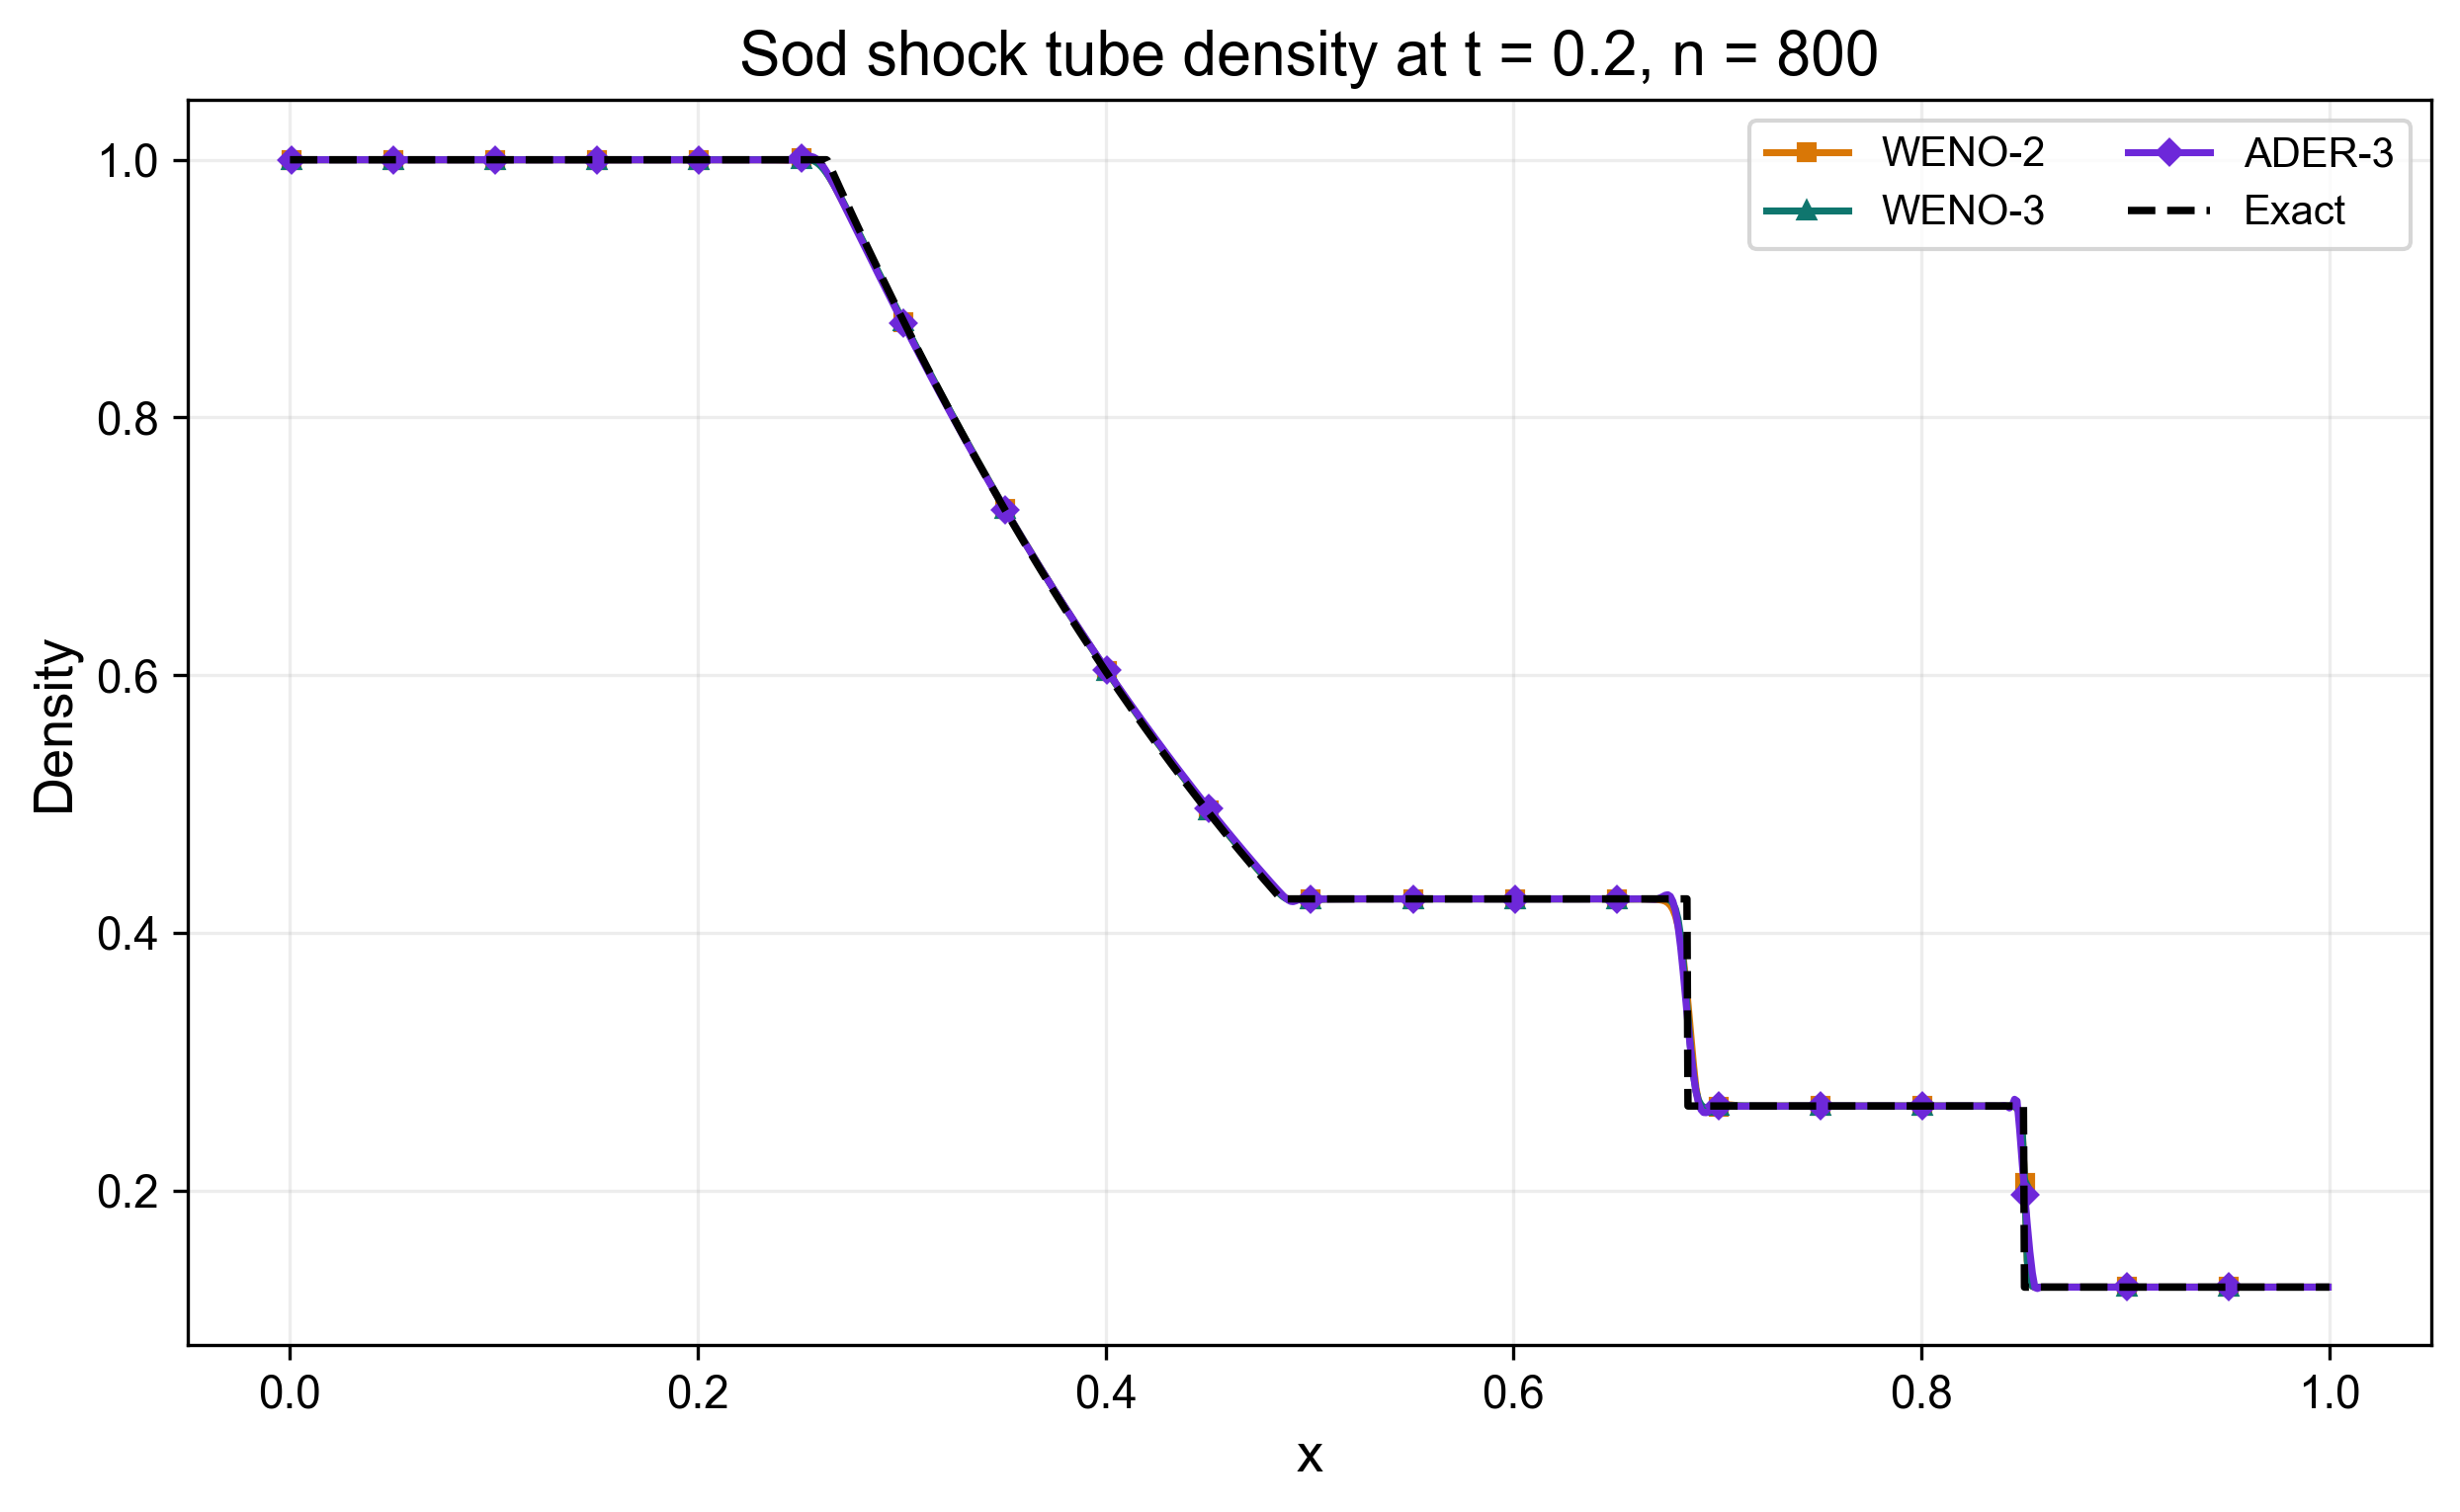
\includegraphics[width=0.91\textwidth]{sod_hllc_n800.png}
\caption{Sod shock-tube density at \(t=0.2\) and \(n=800\). The dashed curve is the exact Riemann solution. Markers are thinned for readability.}
\label{fig:sod-hllc}
\end{figure}

All methods reproduce the rarefaction endpoints, contact and shock locations without a
visible phase error. Their finite thickness is expected for a non-oscillatory finite-volume
solution. Method separation is confined to a few cells around the contact and shock:
WENO-2 gives the broadest transition, while WENO-3 and ADER-3 follow the exact plateaux
more tightly without visible ringing. The recovered contact also verifies the middle-wave
star region in Equation~\eqref{eq:hllcflux} before the analysis moves to interacting
two-dimensional waves.

\section{CFL sensitivity in discontinuous ADER-3}
\label{sec:cfl-study}

The discontinuous ADER-3 calculation required a separate CFL study before the backend comparison could be fixed. This was not a search for a CFL that made one backend appear faster. For every trial, serial and CUDA used the same grid, final time, boundary conditions, HLLC flux and CFL number. The measured quantity was the maximum absolute difference between their exported fields. The two discontinuous problems responded differently because small changes in the accepted time-step sequence can move reconstructed states across an admissibility or troubled-interface threshold.

\begin{table}[H]
\centering
\small
\renewcommand{\arraystretch}{1.18}
\begin{tabular}{@{}ccc>{\raggedright\arraybackslash}p{0.43\textwidth}@{}}
\toprule
CFL & Quadrant Riemann & Shock--bubble & Interpretation \\
\midrule
0.10 & $1.60\times10^{-12}$ & $3.96\times10^{-4}$ & Quadrant stable, shock--bubble branch-sensitive \\
0.12 & $3.36\times10^{-3}$ & $<6\times10^{-8}$ & Shock--bubble stable, quadrant branch-sensitive \\
0.13 & $5.03\times10^{-12}$ & $1.58\times10^{-2}$ & Quadrant stable, shock--bubble mismatch \\
0.14 & $3.68\times10^{-12}$ & $2.02\times10^{-7}$ & Best common compromise \\
0.15 & $4.93\times10^{-12}$ & $\mathcal{O}(10^{-3})$ & Shock--bubble mismatch returns \\
\bottomrule
\end{tabular}
\caption{ADER-3 CFL study used to select the common discontinuous-test value. Entries are the largest absolute CUDA--serial field differences.}
\label{tab:ader3-cfl-study}
\end{table}

The response is non-monotone: reducing CFL does not necessarily reduce the backend difference. A different CFL changes the sequence of accepted time steps, reconstructed interface states and the locations at which the positivity/fallback logic is activated. Values close to a branch threshold can therefore send serial and CUDA through different locally admissible paths even though both calculations remain finite. CFL 0.14 is the only tested common value that keeps the quadrant result near roundoff and the shock--bubble discrepancy below $3\times10^{-7}$. It is consequently used for ADER-3 in all discontinuous backend comparisons. WENO-2 and WENO-3 use CFL 0.20, for which no comparable branch sensitivity was observed.

\FloatBarrier
\section{Two-dimensional physical fields and backend differences}
\label{sec:resolved-fields}

The \(600\times600\) fields below provide the physical reference at a resolution high
enough to expose smooth peaks, shocks and contacts clearly. Backend differences are
measured separately at \(100\times100\), where complete serial, OpenMP and CUDA fields
are compared cell by cell. The two resolutions serve different purposes: the former shows
what was resolved, whereas the latter isolates implementation-dependent differences at
manageable storage cost.

\subsection*{Gaussian advection}

\begin{figure}[!htbp]
\centering
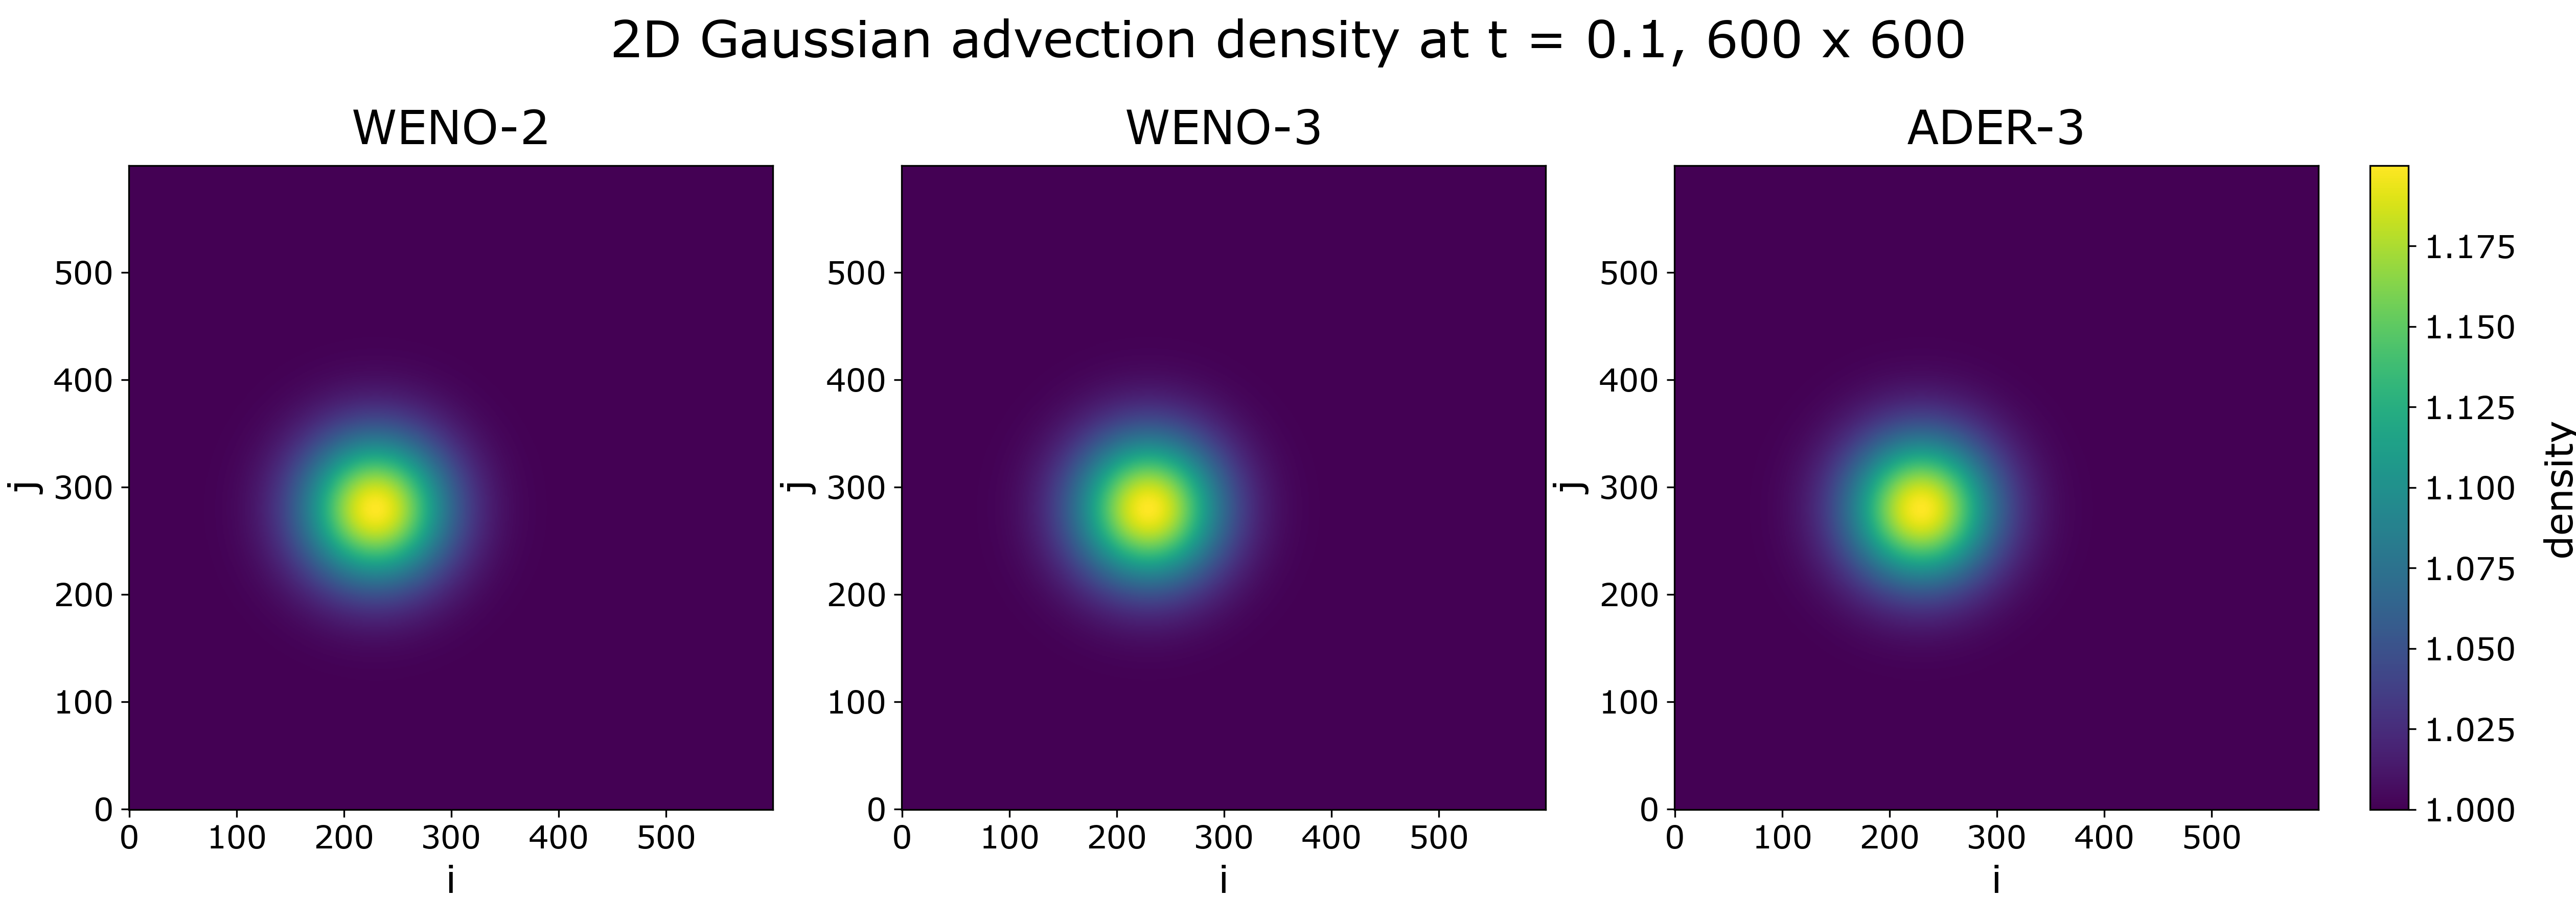
\includegraphics[width=0.98\textwidth]{gaussian_advection_hllc_n600.png}
\caption{HLLC density fields for two-dimensional Gaussian advection at \(t=0.1\) and
\(600\times600\). All methods transport the pulse to the same location and preserve a
smooth, symmetric field. WENO-3 and ADER-3 retain a slightly more compact peak than
WENO-2.}
\label{fig:gaussian-fields-performance}
\end{figure}

Figure~\ref{fig:gaussian-fields-performance} establishes the smooth-flow reference:
the transported pulse is neither displaced nor visibly distorted. On the common colour
scale, WENO-2 has a slightly broader radial footprint, whereas WENO-3 and ADER-3 retain
a more compact peak. All three remain circular, with no directional wake or grid-aligned
deformation. The backend-difference maps below are therefore interpreted against an
unchanged physical solution.

\begin{figure}[!htbp]
\centering
\begin{subfigure}[t]{0.47\textwidth}
\centering
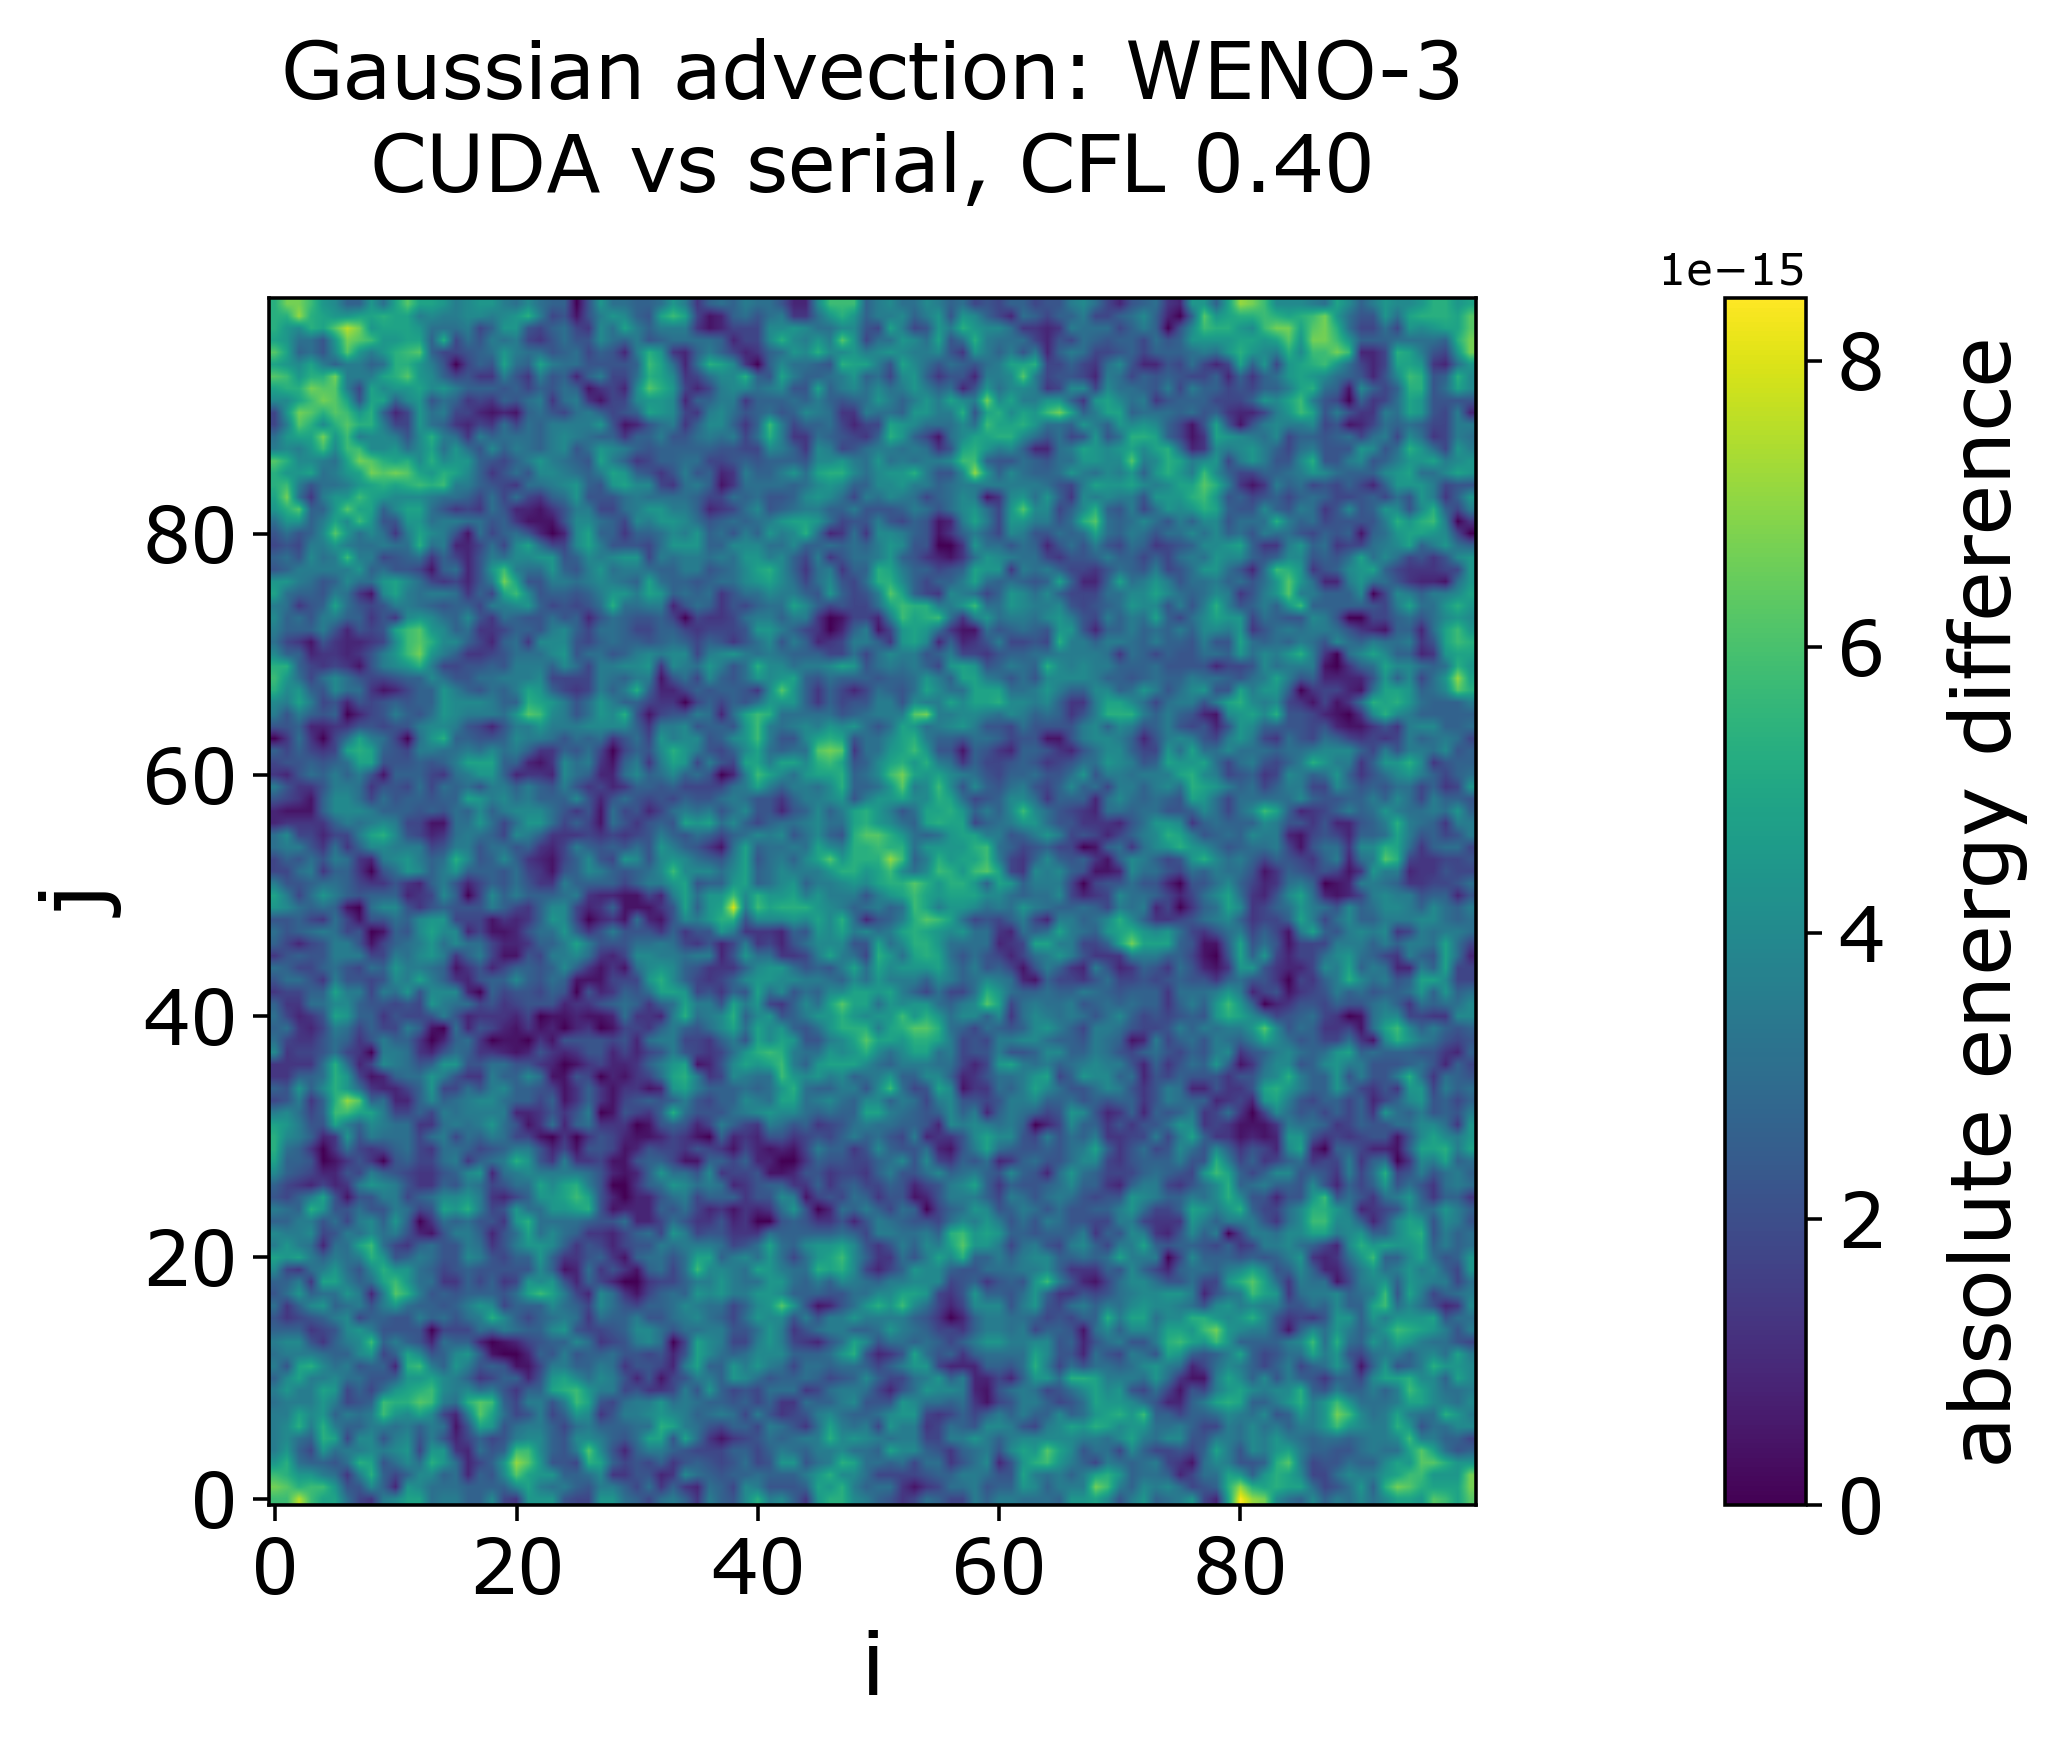
\includegraphics[width=\linewidth]{gaussian_advection_weno3_energy_absdiff.png}
\caption{WENO-3: $\max|\Delta E|=8.438\times10^{-15}$.}
\end{subfigure}\hfill
\begin{subfigure}[t]{0.47\textwidth}
\centering
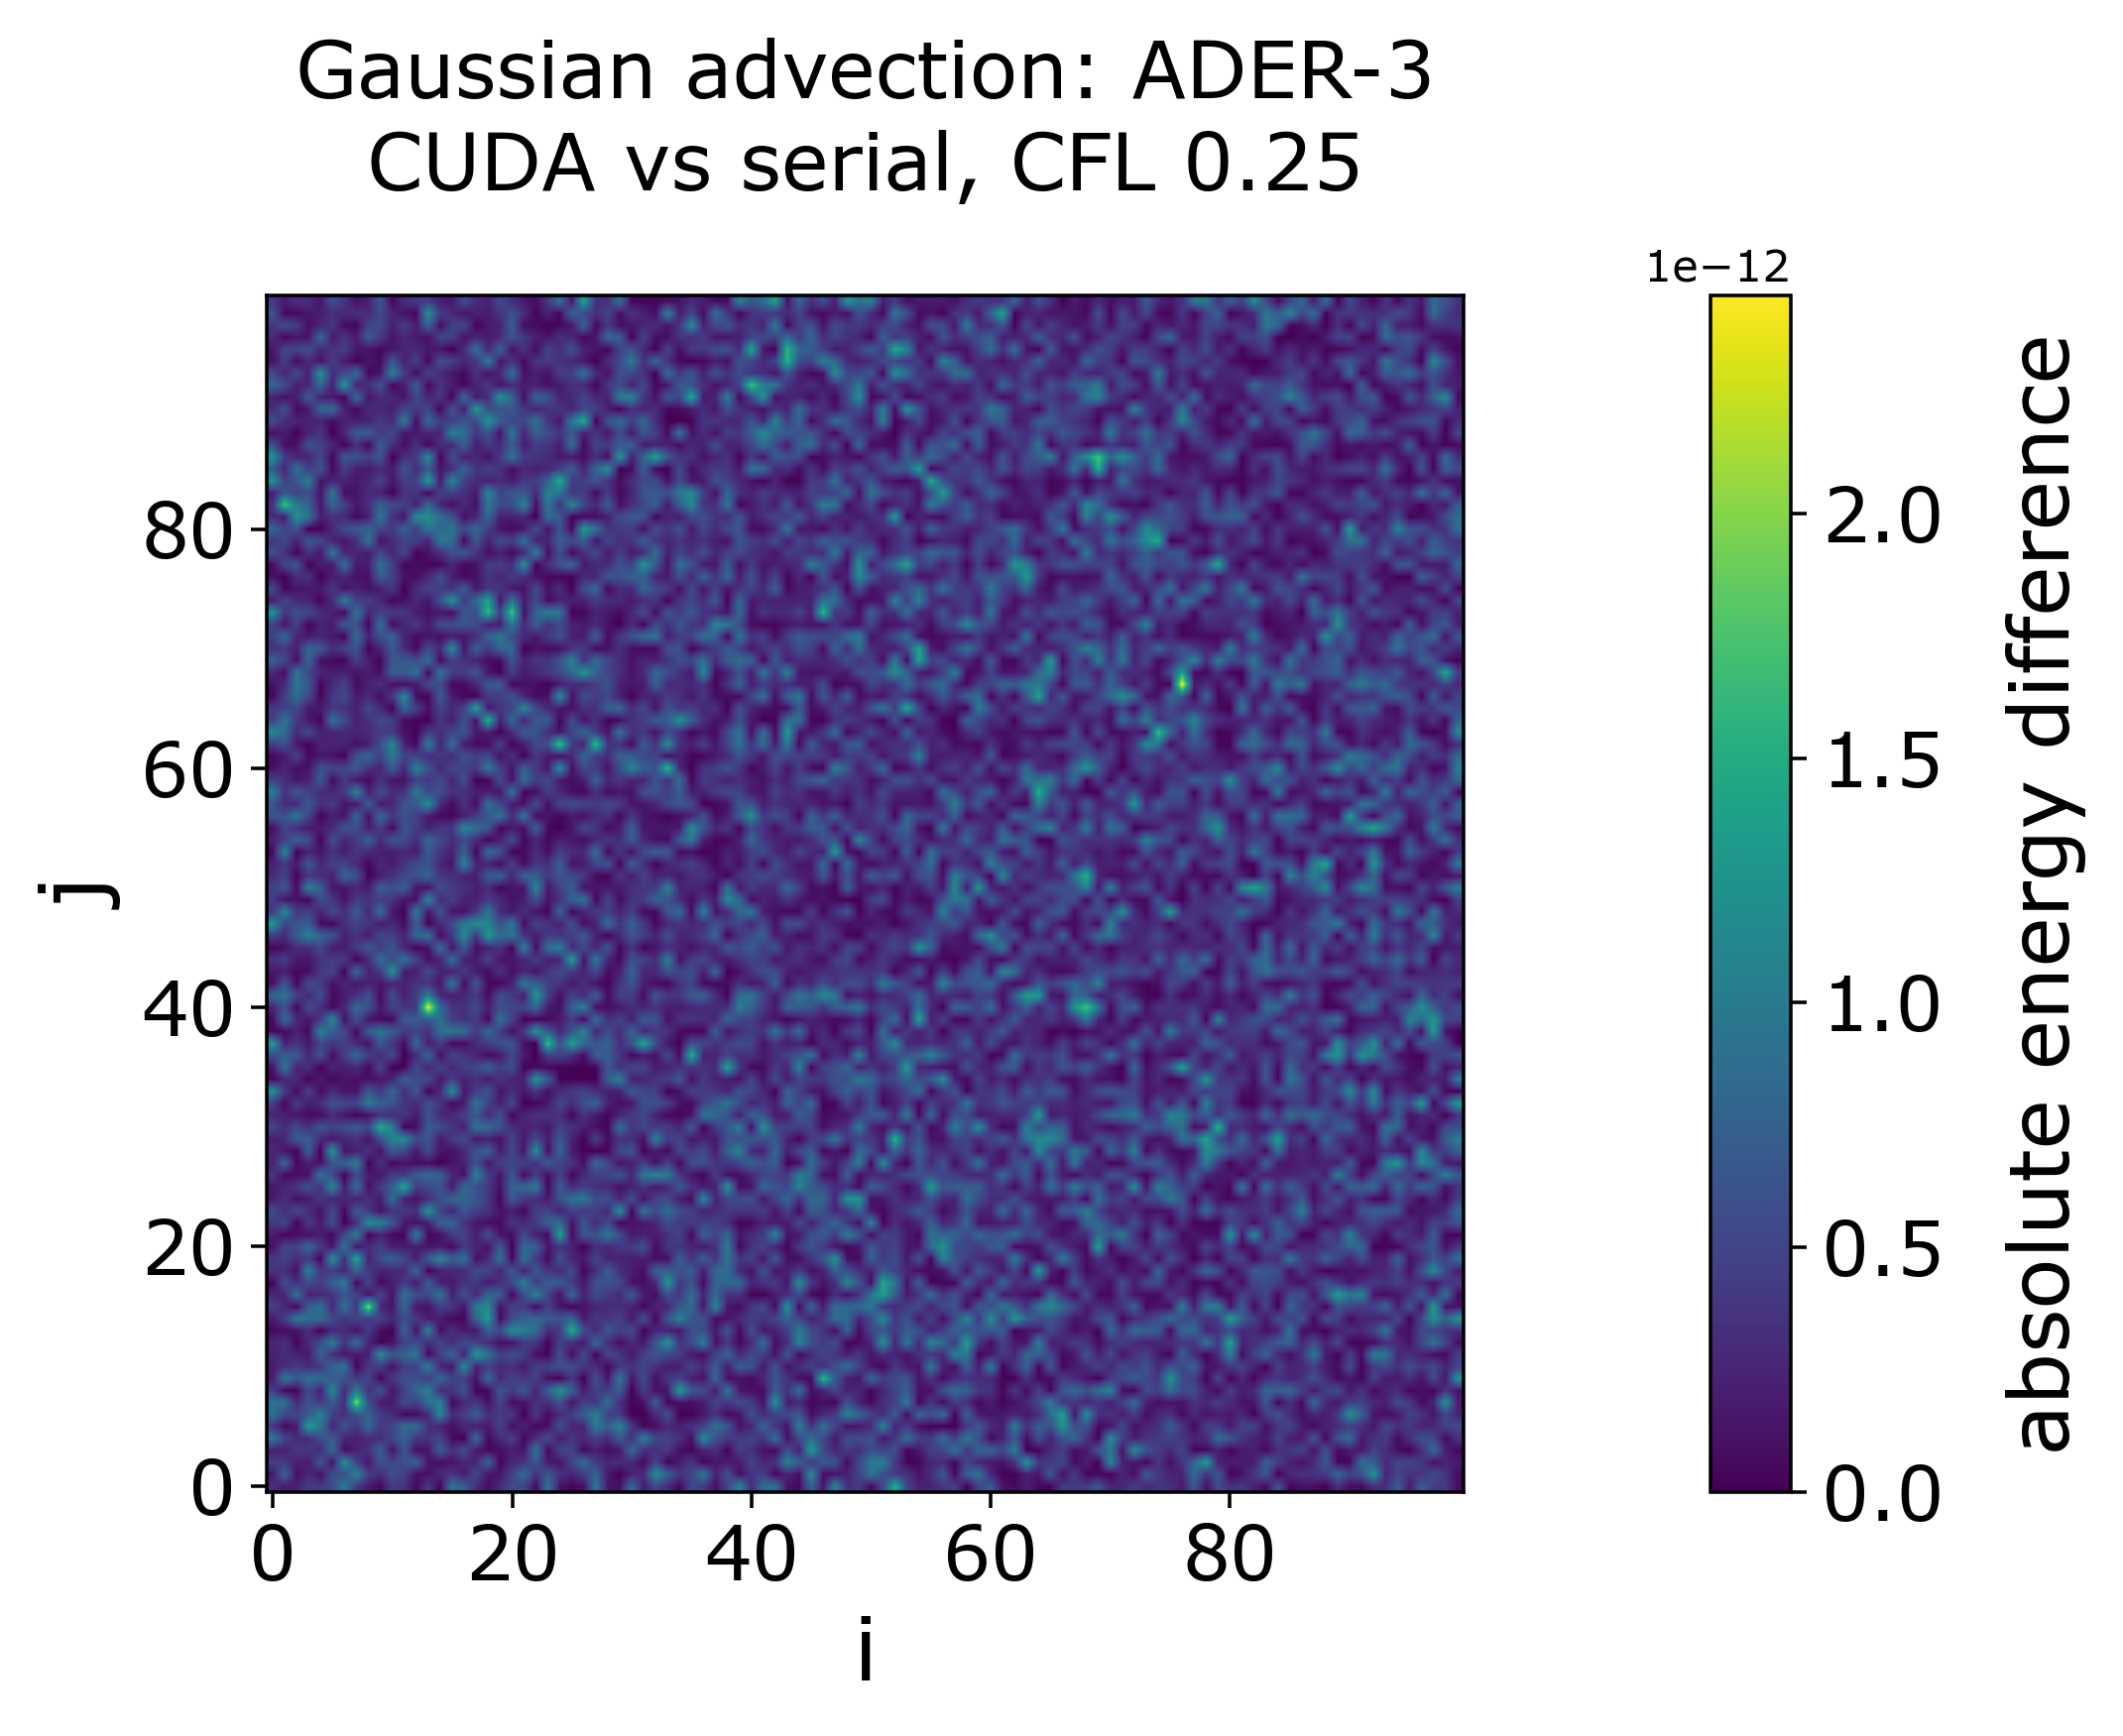
\includegraphics[width=\linewidth]{gaussian_advection_ader3_energy_absdiff.png}
\caption{ADER-3: $\max|\Delta E|=2.445\times10^{-12}$.}
\end{subfigure}
\caption{Absolute CUDA--serial energy differences for Gaussian advection at $100\times100$. Each panel uses its own colour scale.}
\label{fig:third-order-gaussian-difference}
\end{figure}

The absolute differences are extremely small. WENO-3 remains at
$8.438\times10^{-15}$, while the larger ADER-3 energy difference is
$2.445\times10^{-12}$. Both are many orders of magnitude below the resolved density
variation.

Neither map contains a coherent pulse-aligned pattern. Their domain-wide, fine-scale
distribution is characteristic of accumulated floating-point roundoff rather than a
displaced Gaussian pulse, an incorrect boundary treatment, or a backend-dependent
physical branch.

\FloatBarrier
\subsection*{Quadrant Riemann problem}

The quadrant problem contains several waves that meet near the initial intersection, so
reconstruction, HLLC branch selection and multidimensional coupling act in one compact
region. Figure~\ref{fig:quadrant-evolution-discontinuous} first follows a representative
WENO-3 calculation. The four initial constant states begin to interact by \(t=0.1\).
at \(t=0.2\), the central structure is fully developed while regions beyond the wave
fronts retain their prescribed far-field values.

\begin{figure}[!htbp]
\centering
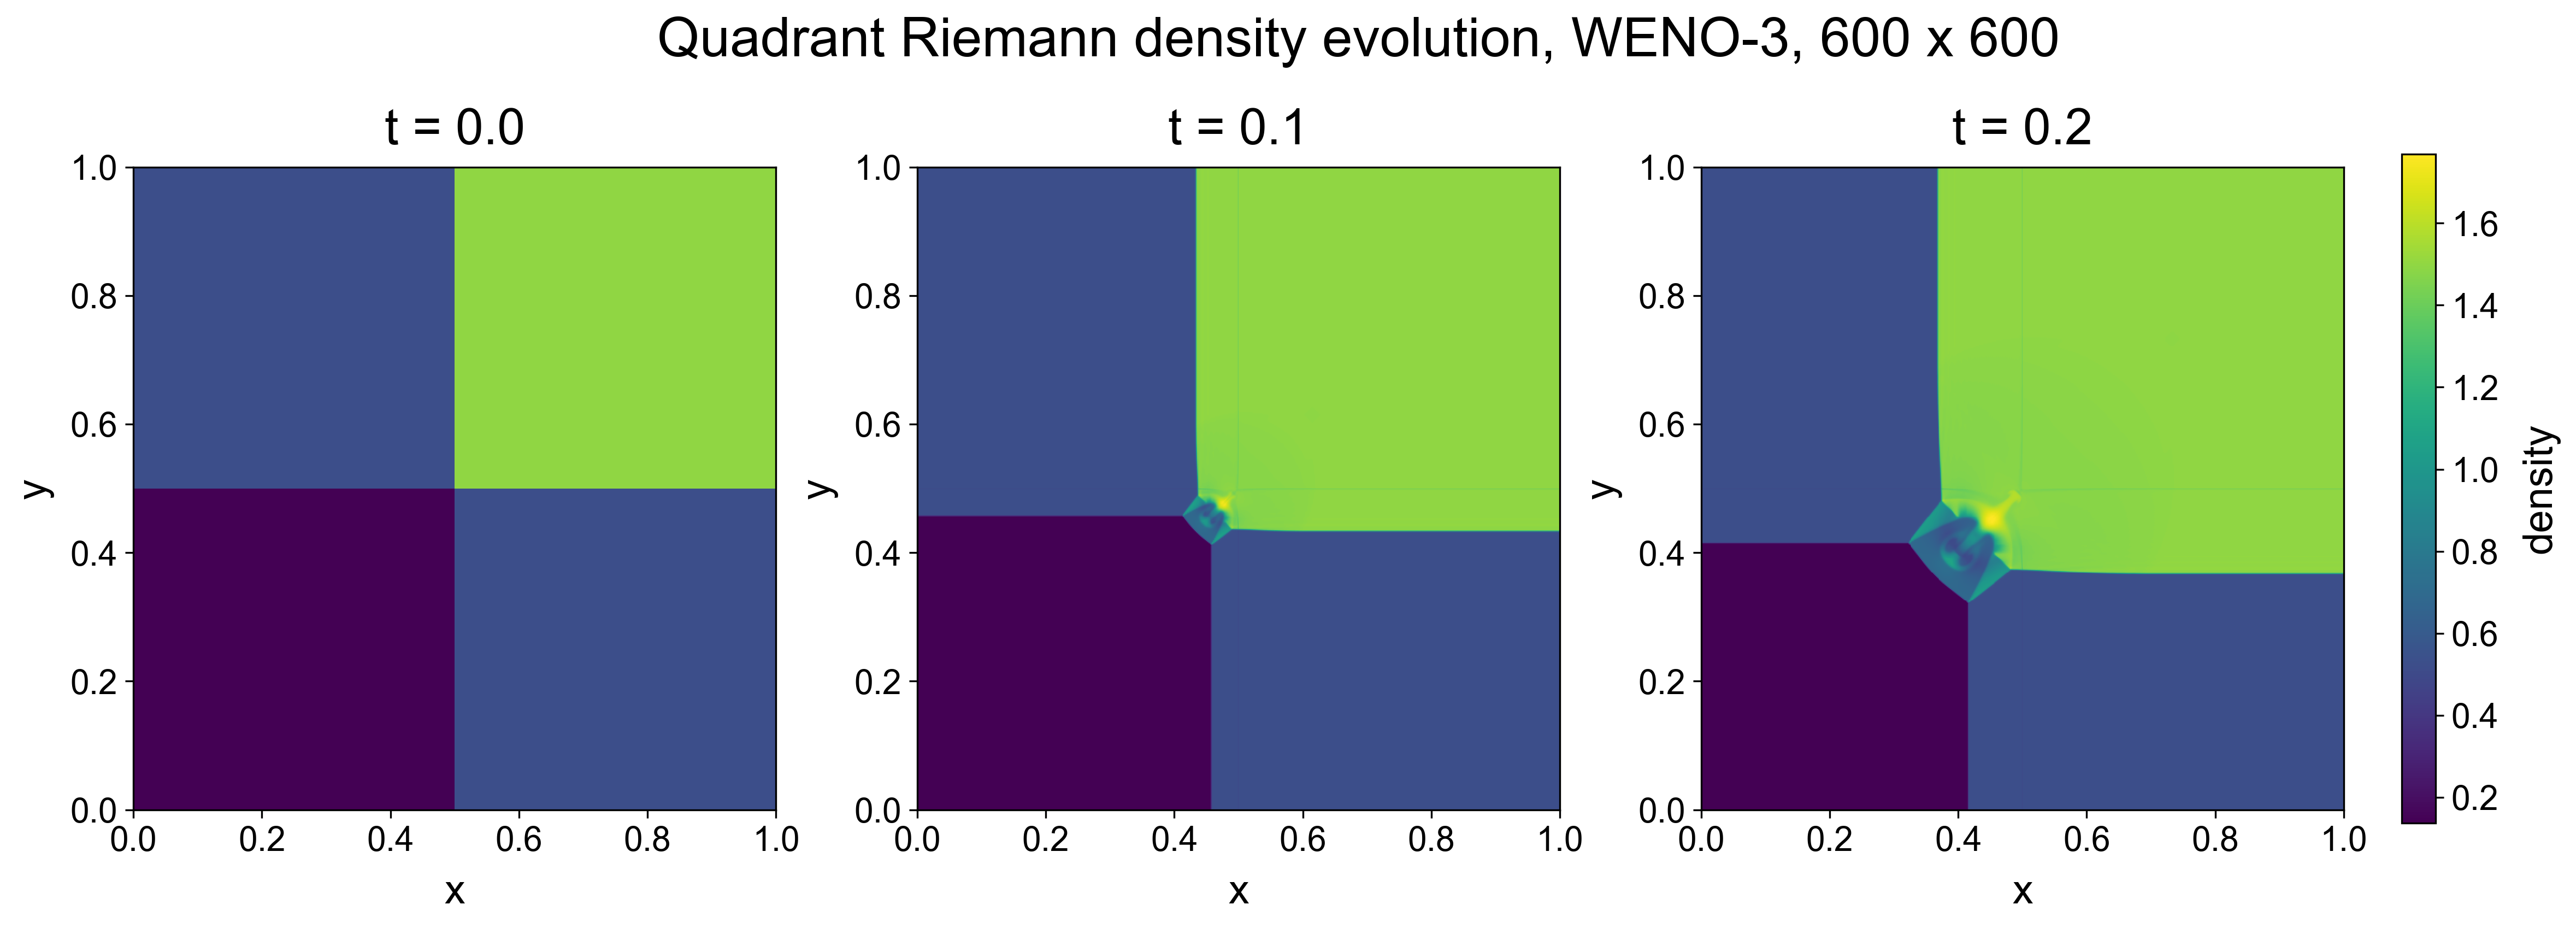
\includegraphics[width=0.98\textwidth]{quadrant_riemann_weno3_evolution_n600.png}
\caption{Density evolution in the \(600\times600\) HLLC WENO-3 quadrant Riemann
calculation. A common colour scale is used at \(t=0\), \(0.1\), and \(0.2\).}
\label{fig:quadrant-evolution-discontinuous}
\end{figure}

Figure~\ref{fig:quadrant-evolution-discontinuous} establishes the temporal development.
Figure~\ref{fig:quadrant-fields-discontinuous} then fixes the final time and colour scale
to compare method-dependent interface thickness and local extrema.

\begin{figure}[!htbp]
\centering
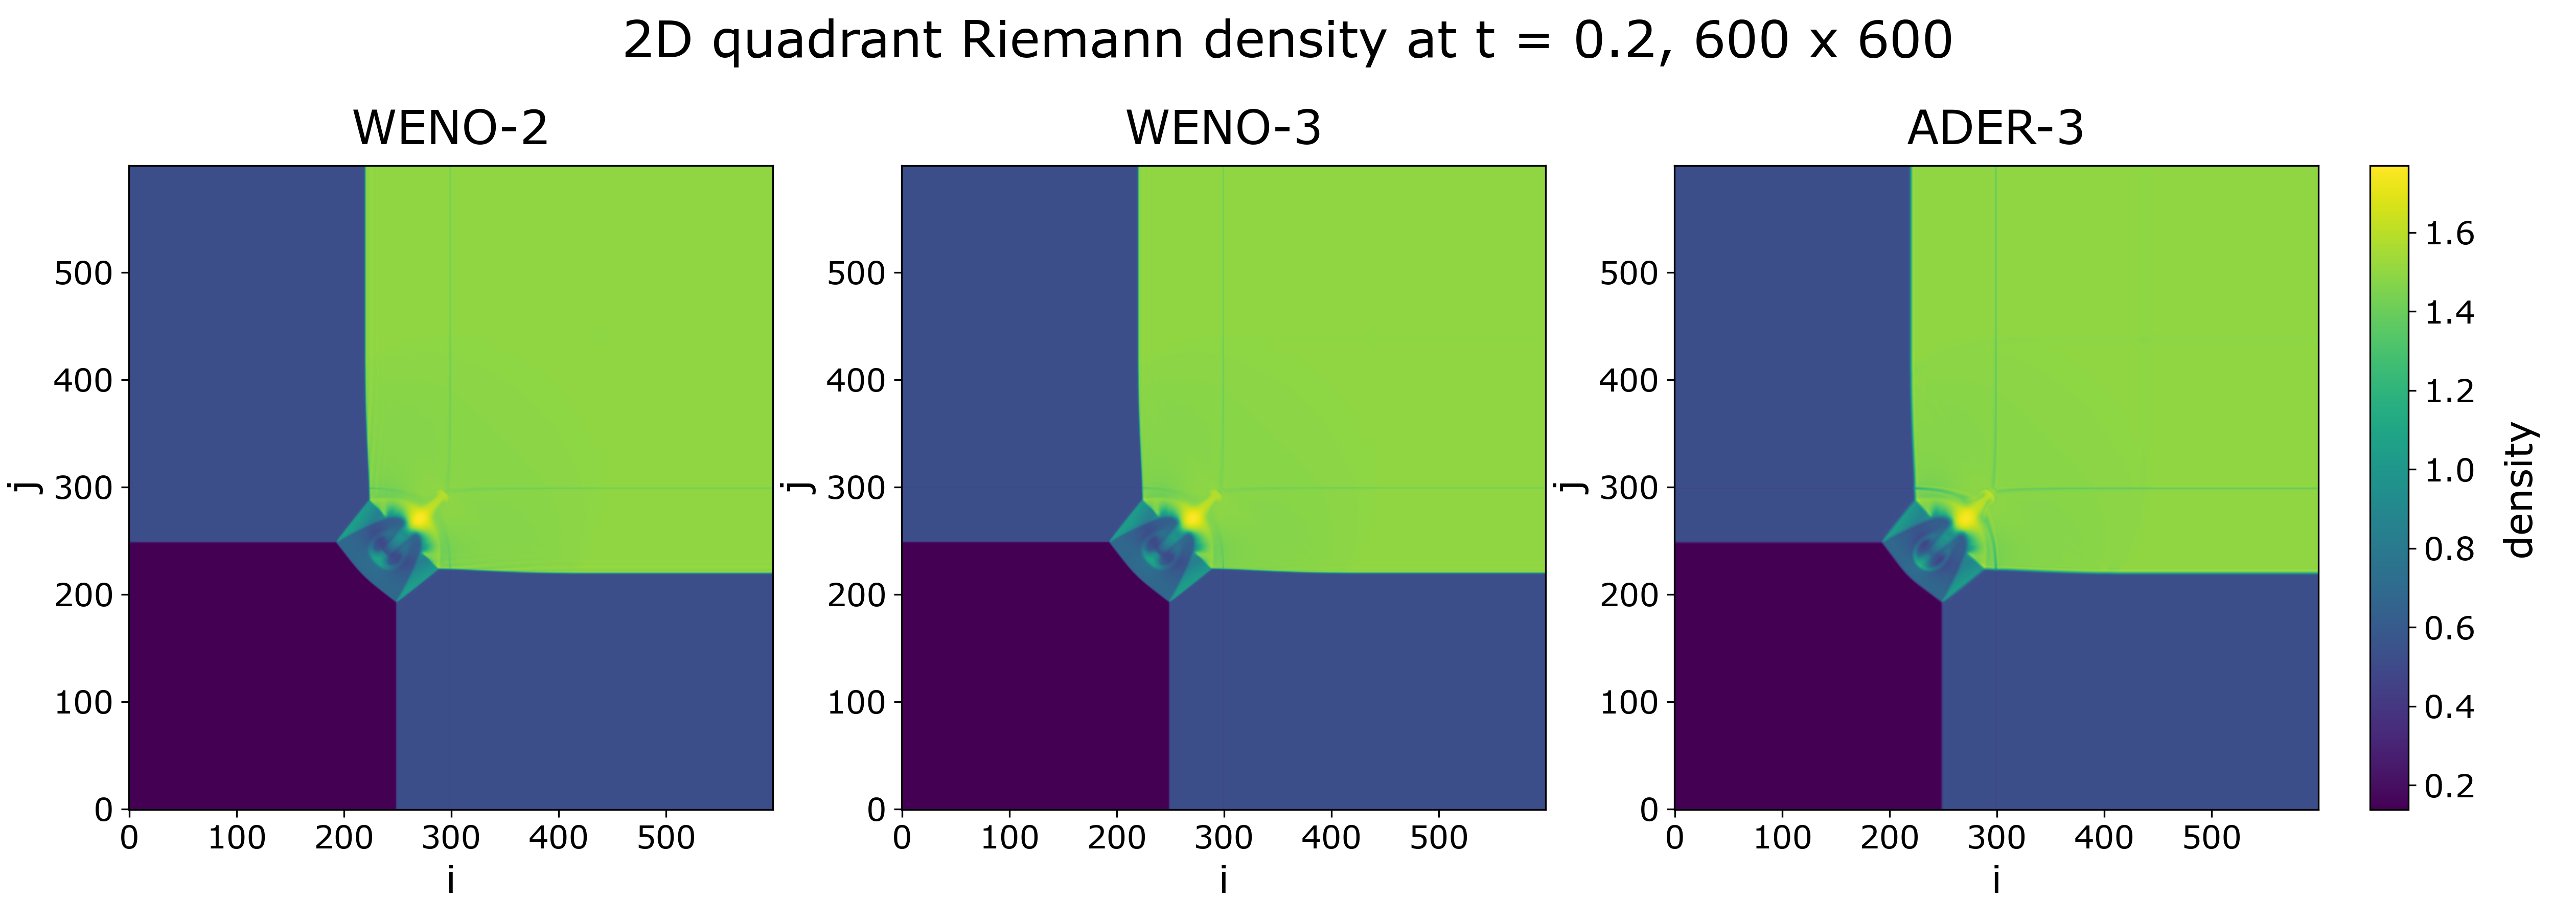
\includegraphics[width=0.98\textwidth]{quadrant_riemann_hllc_n600.png}
\caption{Quadrant Riemann density at \(t=0.2\) and \(600\times600\). Each panel uses
the same colour scale. All methods preserve the four far-field states and resolve the same
large-scale wave pattern. Their differences are concentrated near the compact interaction
region.}
\label{fig:quadrant-fields-discontinuous}
\end{figure}

The three final fields preserve the four far-field states and the same interacting-wave
topology, while their visible differences remain confined to the compact central region.
The off-interface slice in Figure~\ref{fig:quadrant-slice-discontinuous} then gives a more
discriminating comparison: the main jump, intermediate trough and post-interaction plateau
occur at the same coordinates for all three methods.

\begin{figure}[!htbp]
\centering
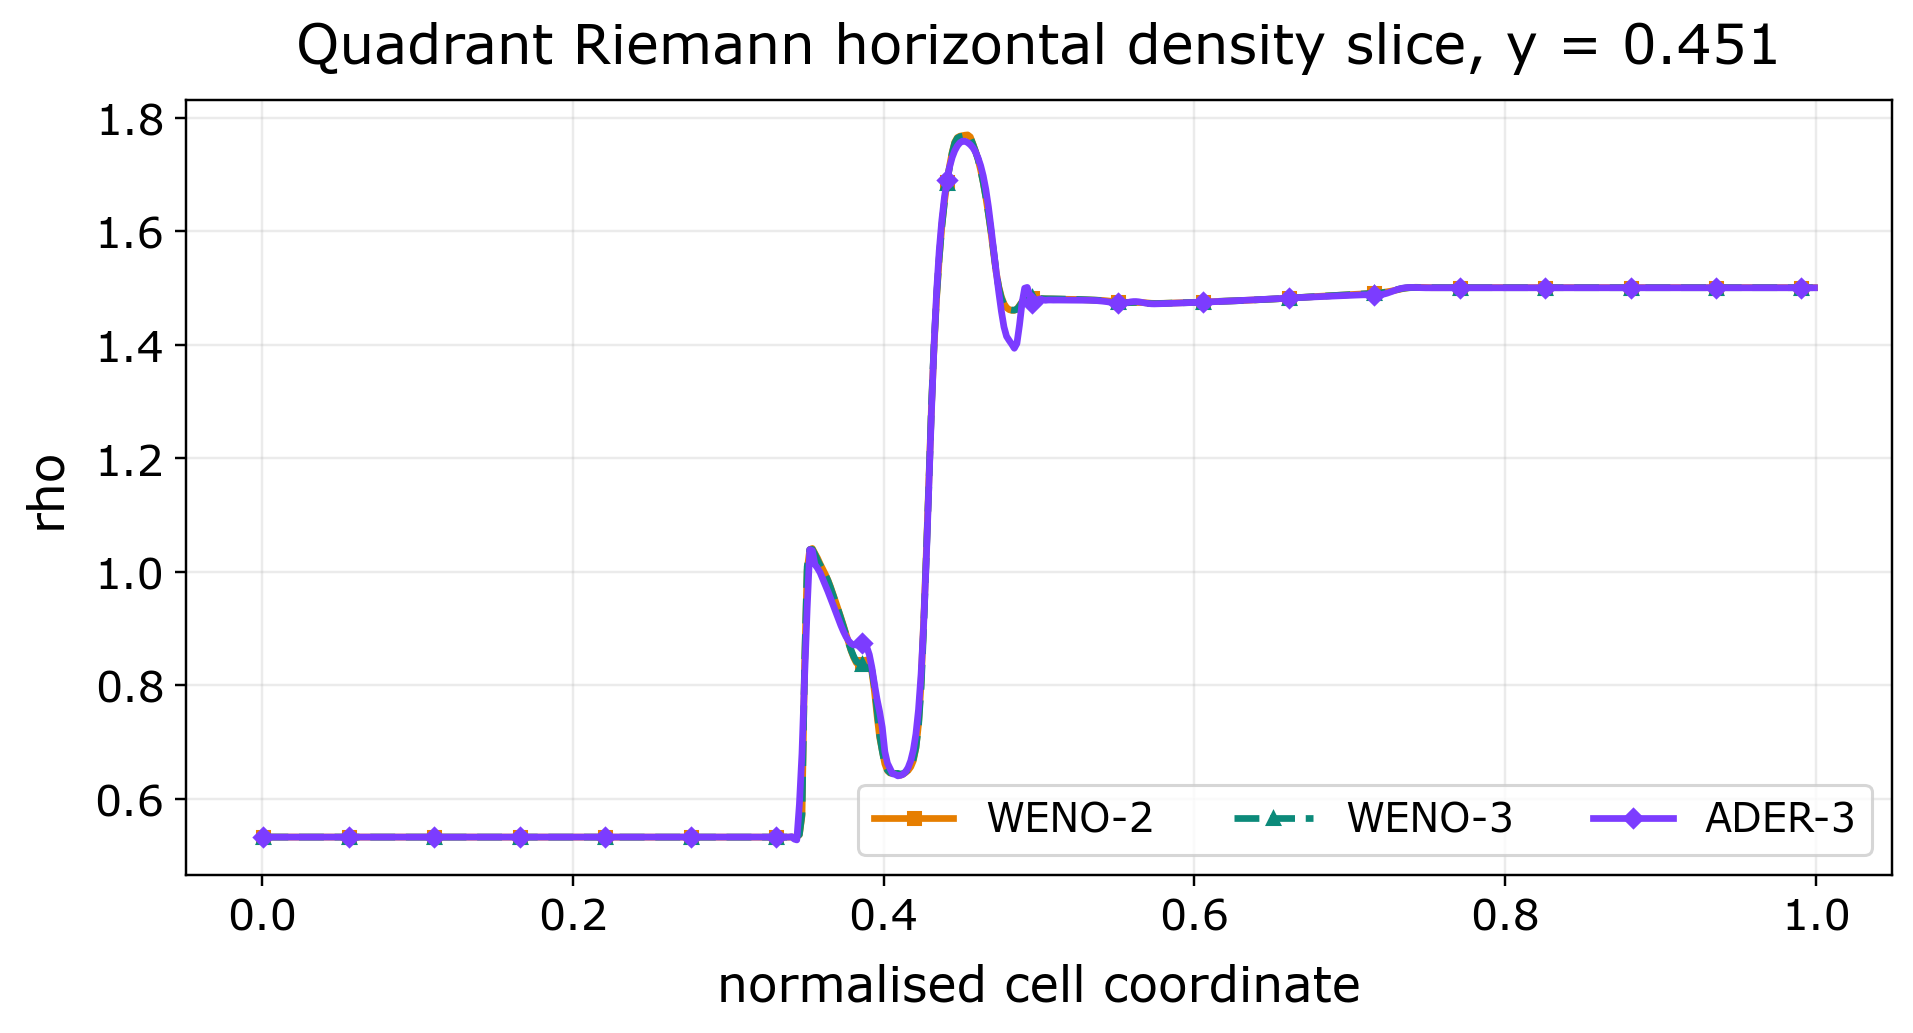
\includegraphics[width=0.90\textwidth]{quadrant_riemann_slice_hllc_n600.png}
\caption{Quadrant Riemann density along \(y=0.451\). Sampling away from the initial
quadrant boundary removes cell-ownership ambiguity while retaining the interacting waves.}
\label{fig:quadrant-slice-discontinuous}
\end{figure}

WENO-3 follows WENO-2 closely but resolves the narrow changes more steeply. ADER-3
captures the same state sequence with a stronger local excursion near the interaction,
where its troubled-interface decision switches between the space--time predictor and
cell-average HLLC fallback. The flat states away from the waves show that these are local
method differences, not an incorrect initial condition. Figure~\ref{fig:third-order-quadrant-difference}
next localises the still smaller backend discrepancies relative to that common solution.

WENO-3 remains near roundoff in energy, whereas the dominant ADER-3
\(x\)-velocity discrepancy reaches $3.679\times10^{-12}$. In both maps the largest
local values follow the discontinuities and central interaction region, where small
backend perturbations encounter the steepest reconstructed gradients.

The WENO-3 map also has a nearly uniform background in the upper-right far-field state.
Its mean energy difference there is approximately \(3.1\times10^{-14}\), compared with
\(2.1\times10^{-16}\) in the lower-left far field. Because the upper-right state has the
largest total-energy magnitude, a higher absolute roundoff floor is expected. The plateau
contains no displaced-wave pattern, while the brighter lines identify local amplification
near discontinuities. Neither feature indicates an incorrect initial condition or a
domain-wide physical displacement.

\begin{figure}[!htbp]
\centering
\begin{subfigure}[t]{0.47\textwidth}
\centering
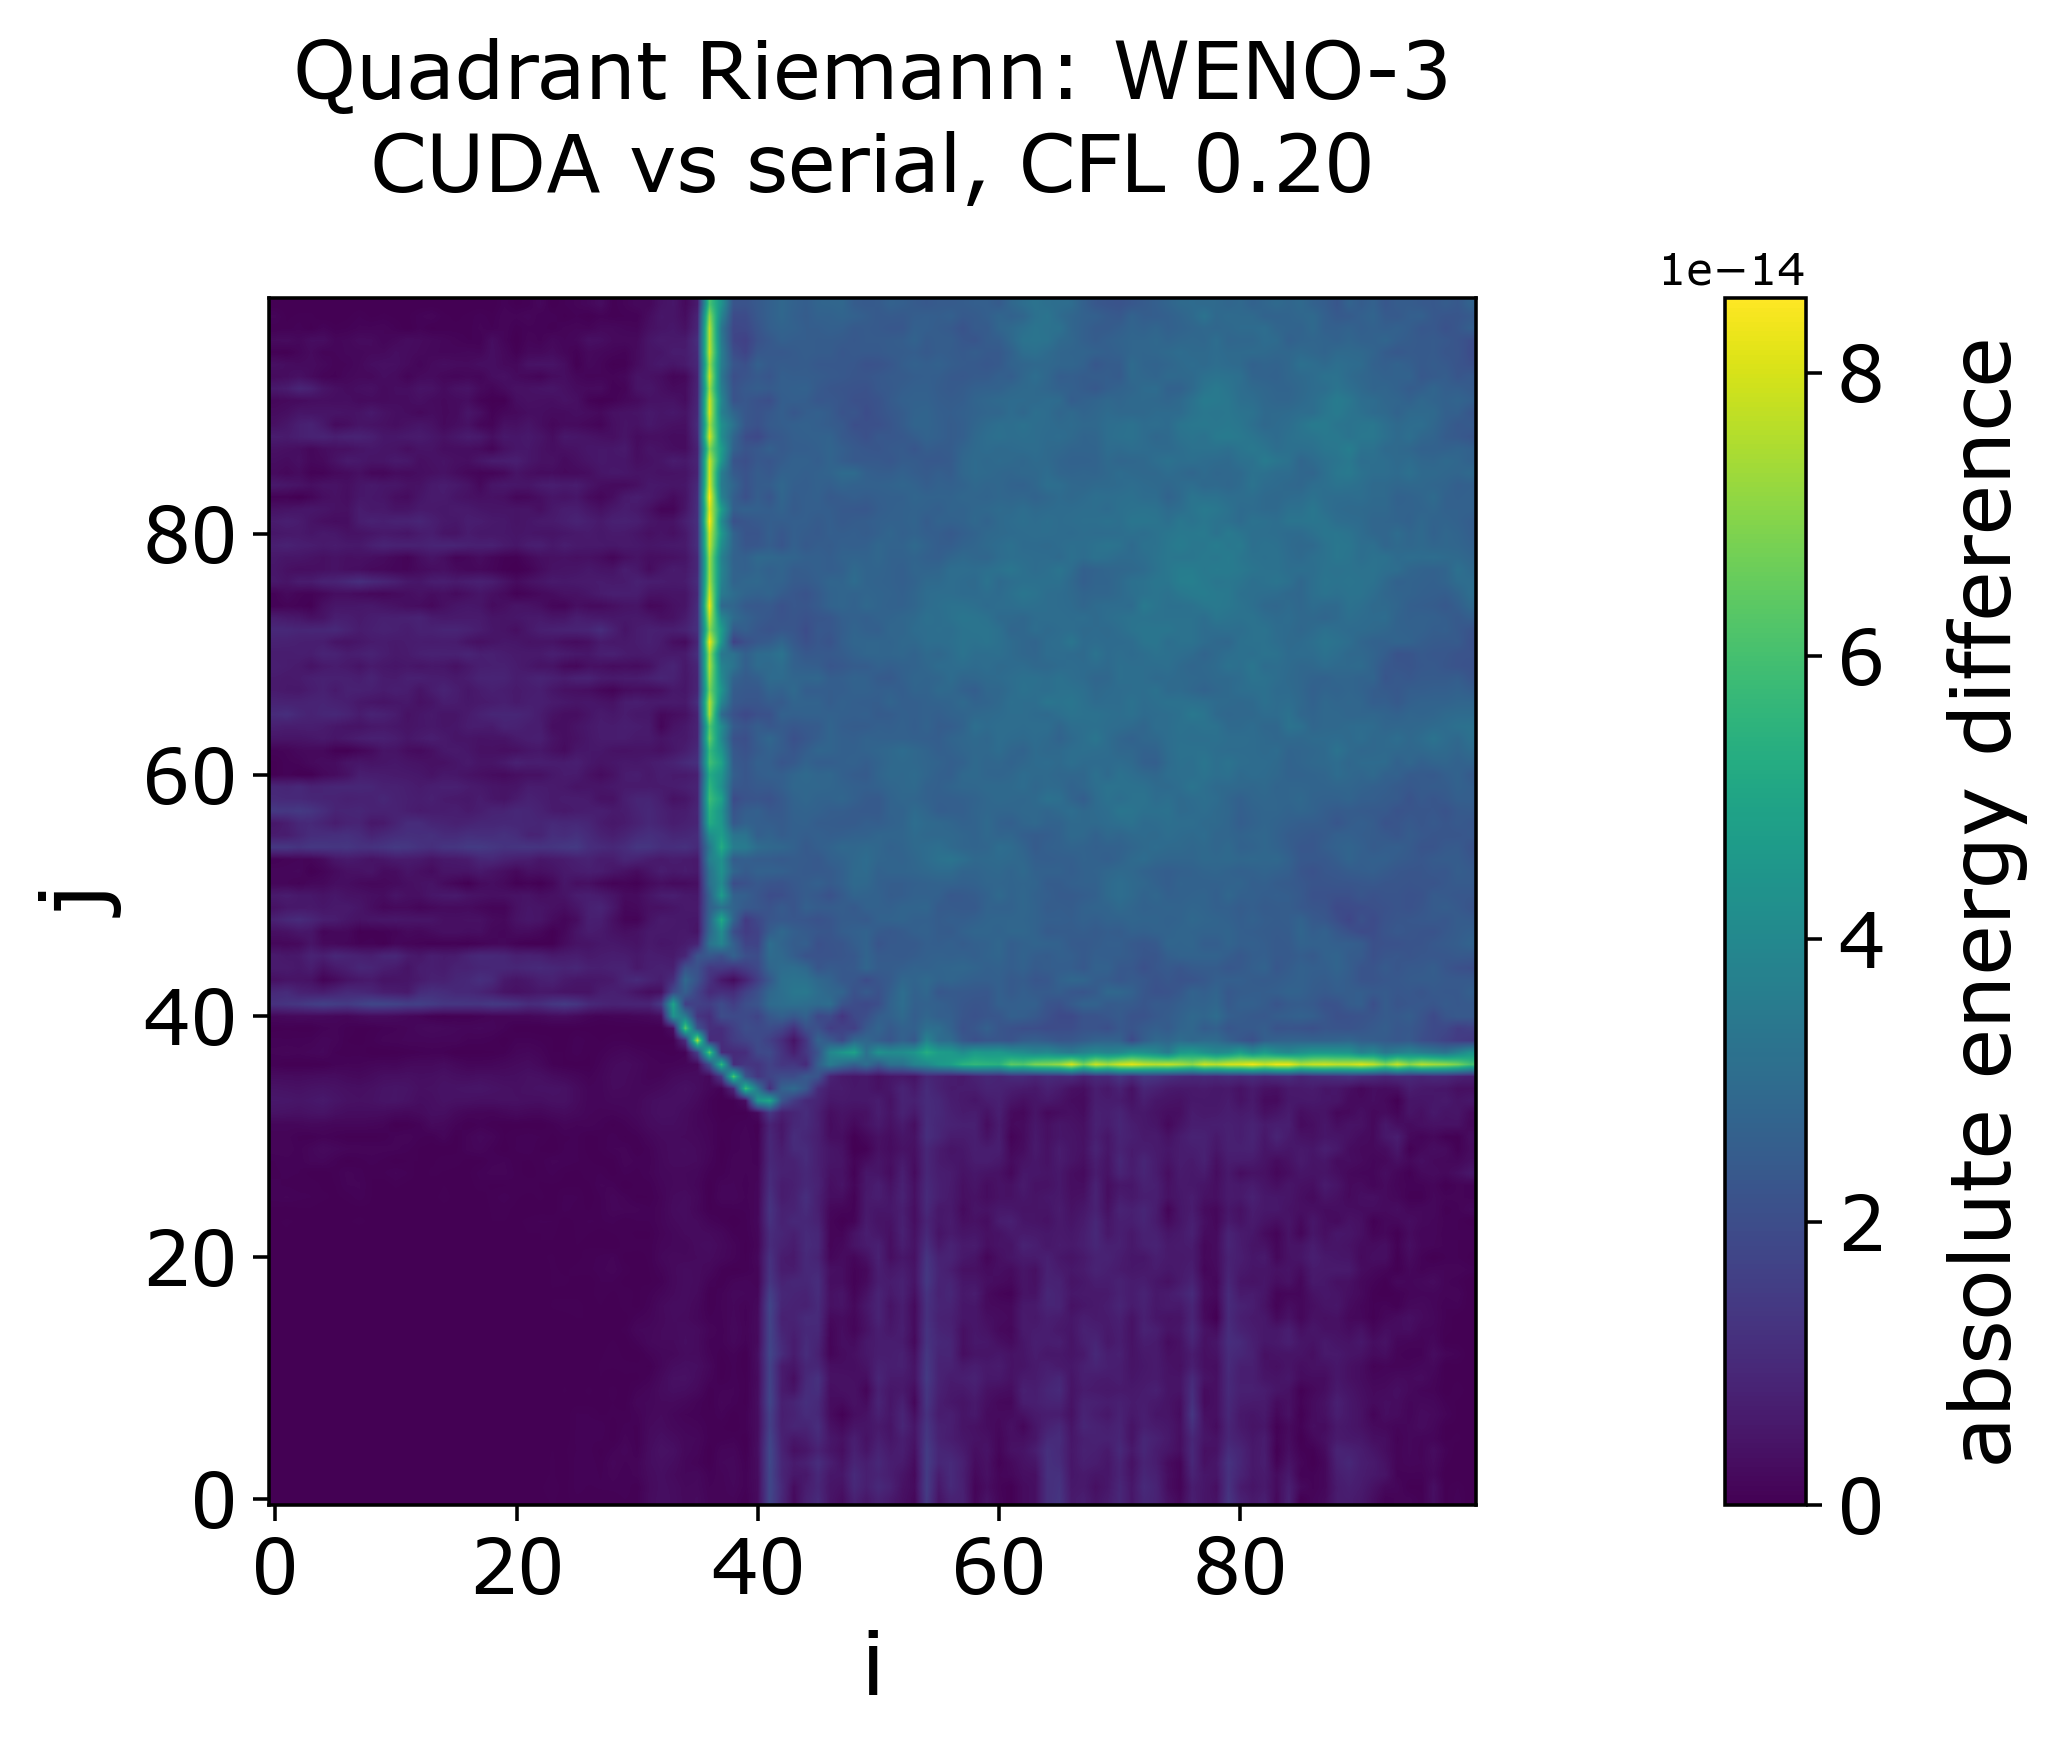
\includegraphics[width=\linewidth]{quadrant_riemann_weno3_energy_absdiff_cfl020.png}
\caption{WENO-3, CFL 0.20: $\max|\Delta E|=8.527\times10^{-14}$.}
\end{subfigure}\hfill
\begin{subfigure}[t]{0.47\textwidth}
\centering
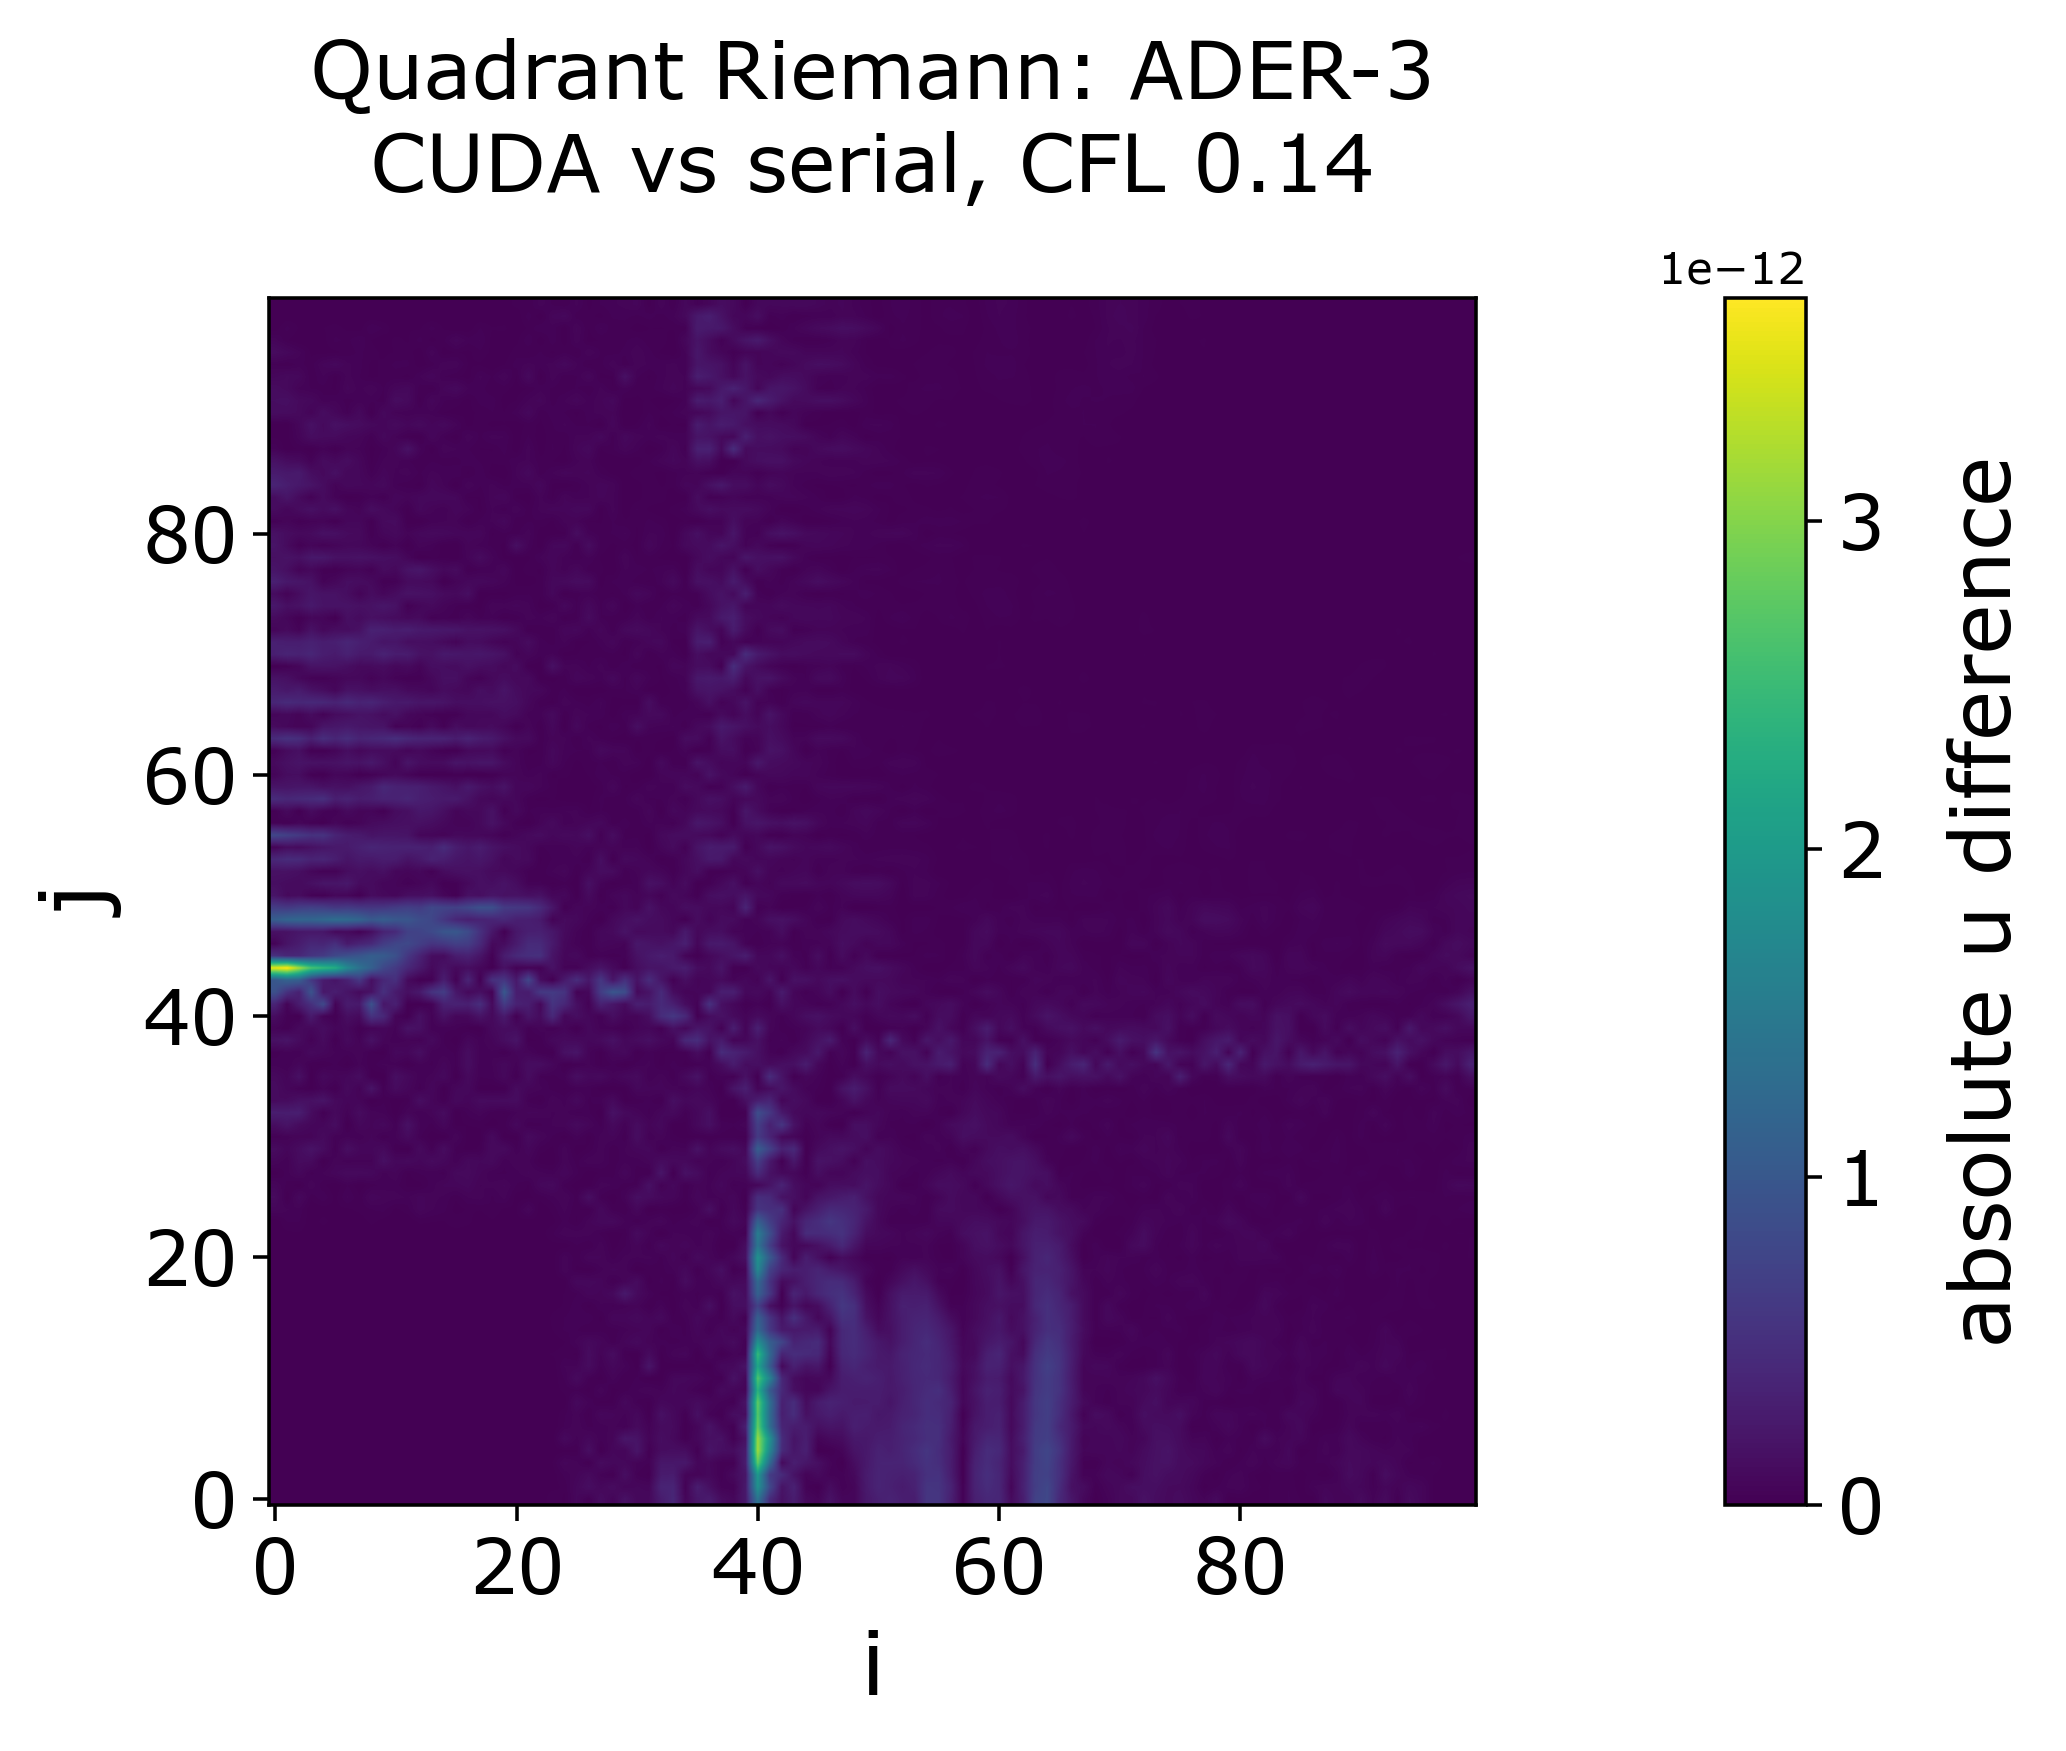
\includegraphics[width=\linewidth]{quadrant_riemann_ader3_u_absdiff_cfl014.png}
\caption{ADER-3, CFL 0.14: $\max|\Delta u|=3.679\times10^{-12}$.}
\end{subfigure}
\caption{Absolute CUDA--serial differences for the quadrant Riemann problem at
$100\times100$. The plotted variable is the dominant field for each method and each panel
uses its own colour scale.}
\label{fig:third-order-quadrant-difference}
\end{figure}

\FloatBarrier
\subsection*{Shock--bubble interaction}

This test is especially relevant to HLLC because the low-density bubble is bounded by a
curved contact. Figure~\ref{fig:shock-evolution-discontinuous} separates the main stages:
a planar shock approaches the bubble at \(t=0\), enters and deforms it by \(t=0.1\), and
leaves reflected and transmitted waves around a distorted low-density region at \(t=0.2\).

\begin{figure}[!htbp]
\centering
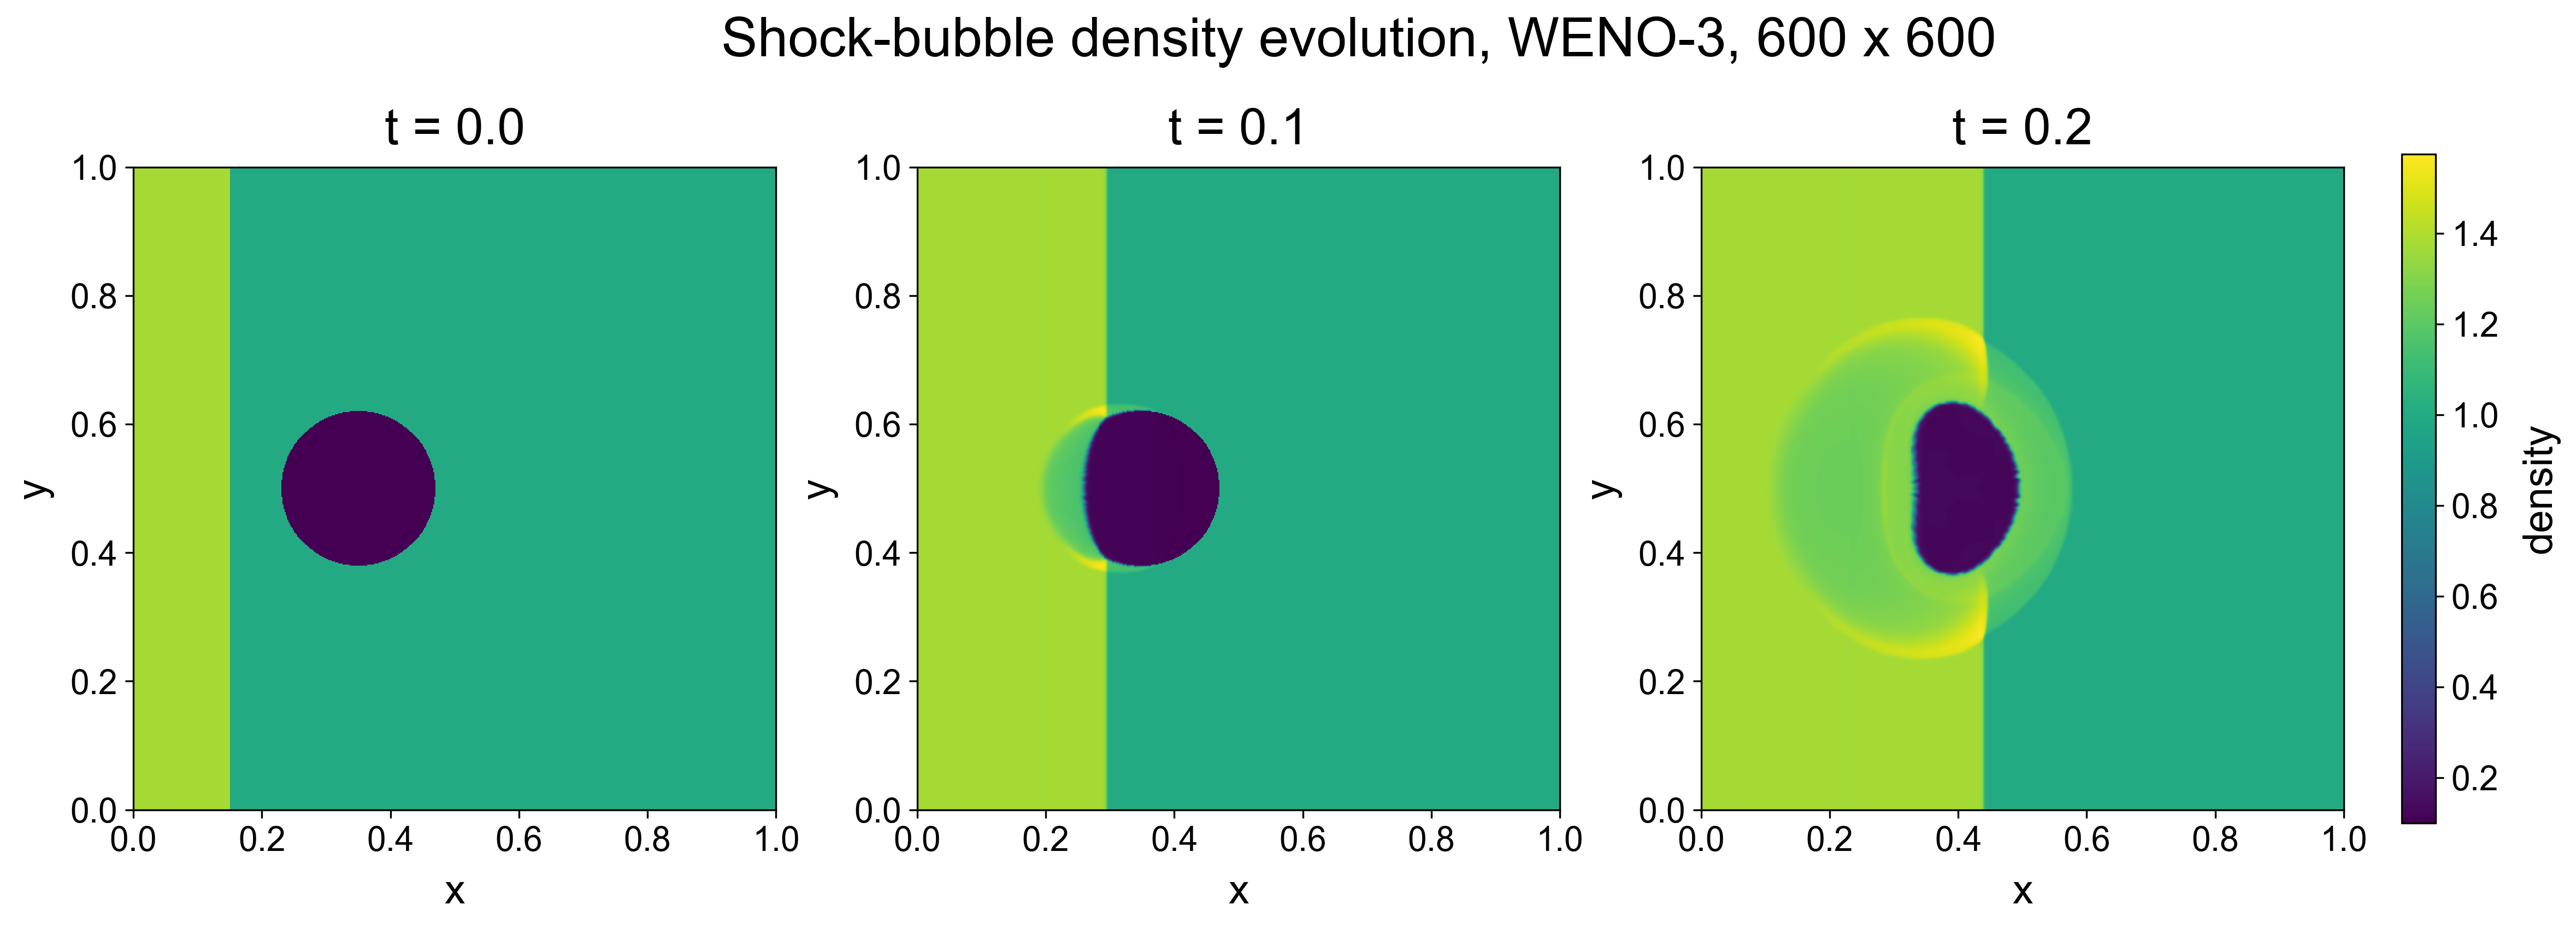
\includegraphics[width=0.98\textwidth]{shock_bubble_weno3_evolution_n600.png}
\caption{Density evolution in the \(600\times600\) HLLC WENO-3 shock--bubble
calculation. The panels at \(t=0\), \(0.1\), and \(0.2\) use one common colour scale.}
\label{fig:shock-evolution-discontinuous}
\end{figure}

The evolution sequence identifies approach, impact and post-interaction deformation.
Figure~\ref{fig:shock-fields-discontinuous} then fixes \(t=0.2\) and the colour scale to
compare numerical diffusion and contact resolution across the three methods.

\begin{figure}[!htbp]
\centering
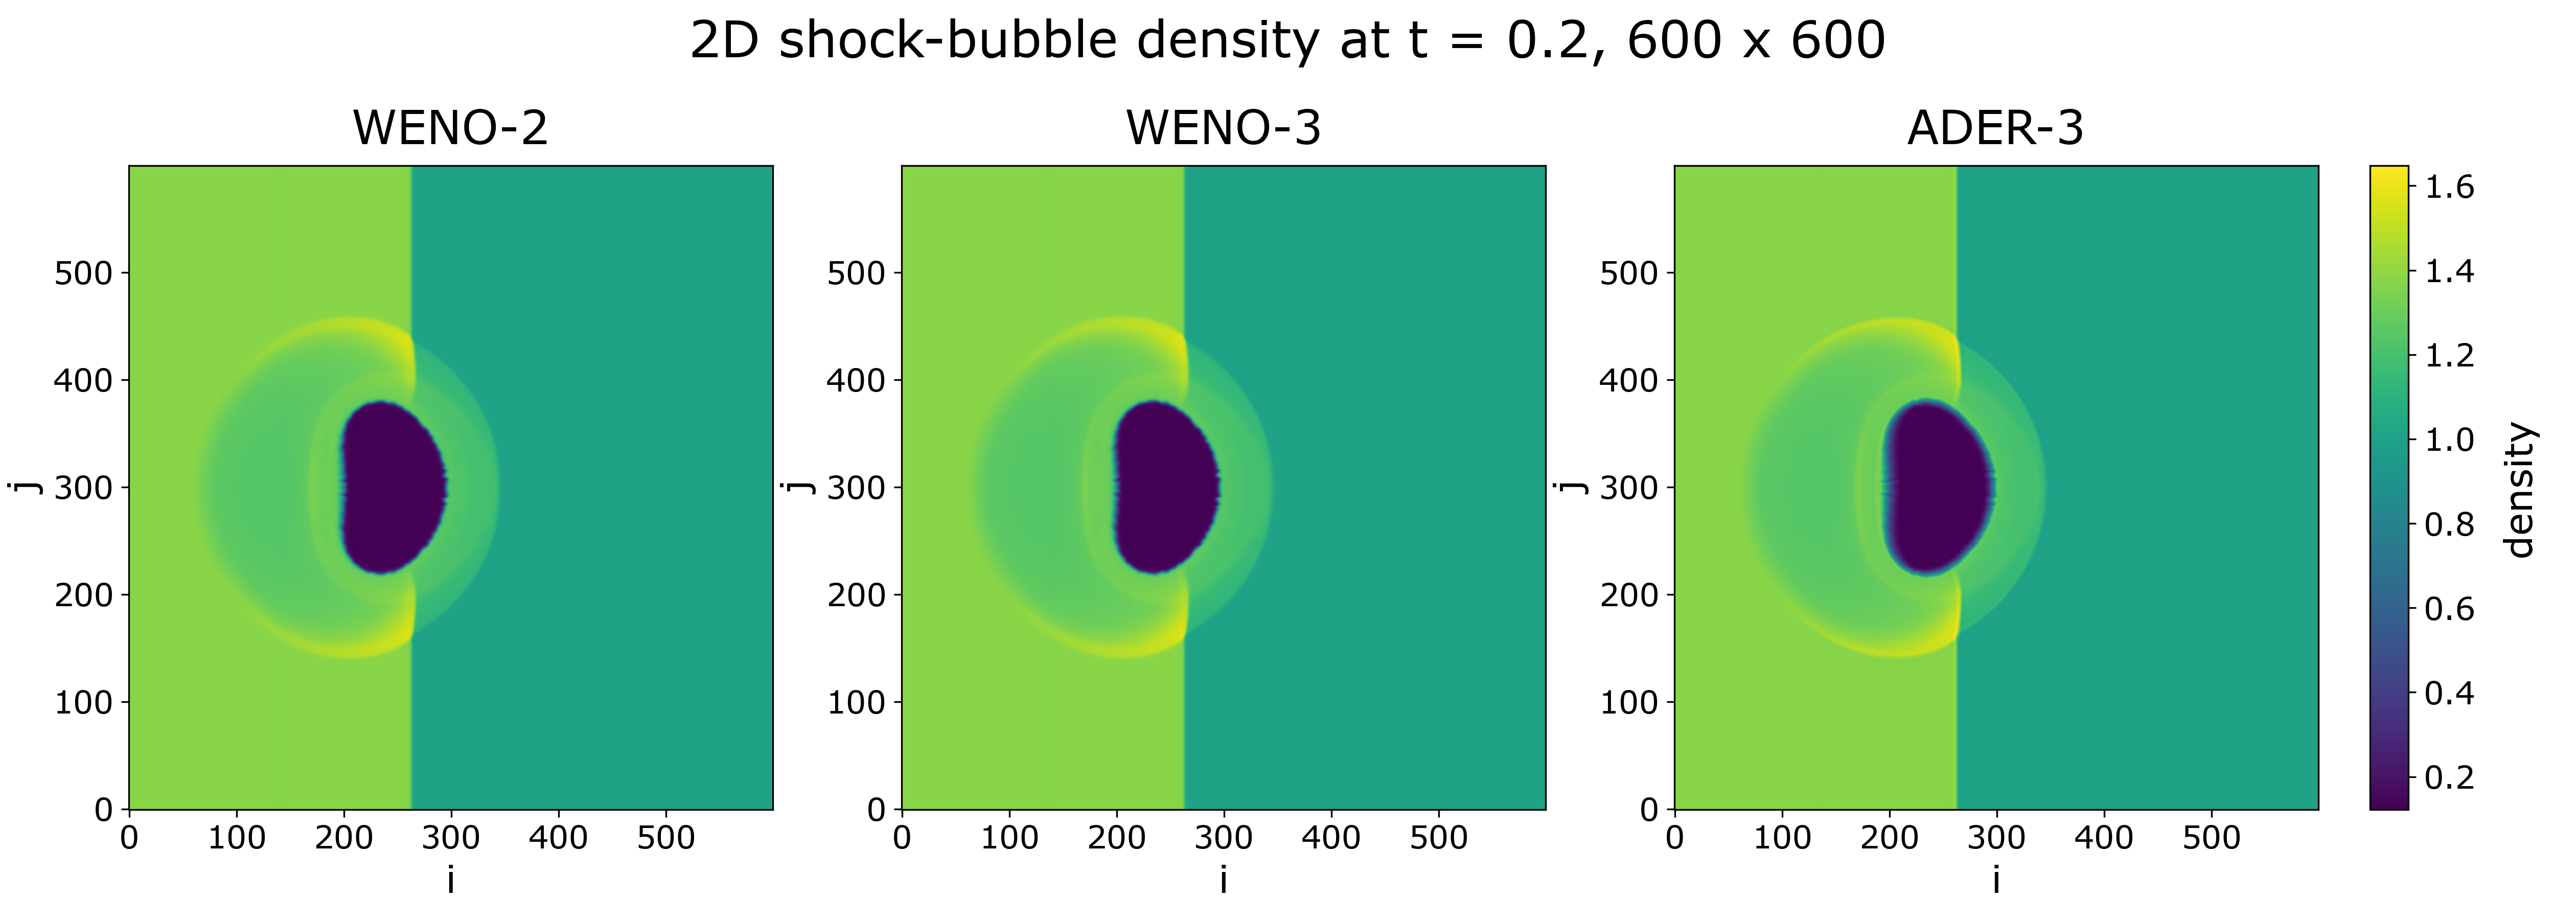
\includegraphics[width=0.98\textwidth]{shock_bubble_hllc_n600.png}
\caption{Shock--bubble density at \(t=0.2\) and \(600\times600\). The shared colour
scale exposes differences in contact thickness and extrema around the curved bubble:
WENO-2 is the most diffusive, WENO-3 retains a thinner transition, and ADER-3 gives the
strongest local contrast.}
\label{fig:shock-fields-discontinuous}
\end{figure}

All three final fields propagate the incident shock through the bubble and preserve the
expected distorted low-density region. Their differences are concentrated in contact
thickness and nearby extrema, as the centre-near slice in
Figure~\ref{fig:shock-slice-discontinuous} makes explicit.

\begin{figure}[!htbp]
\centering
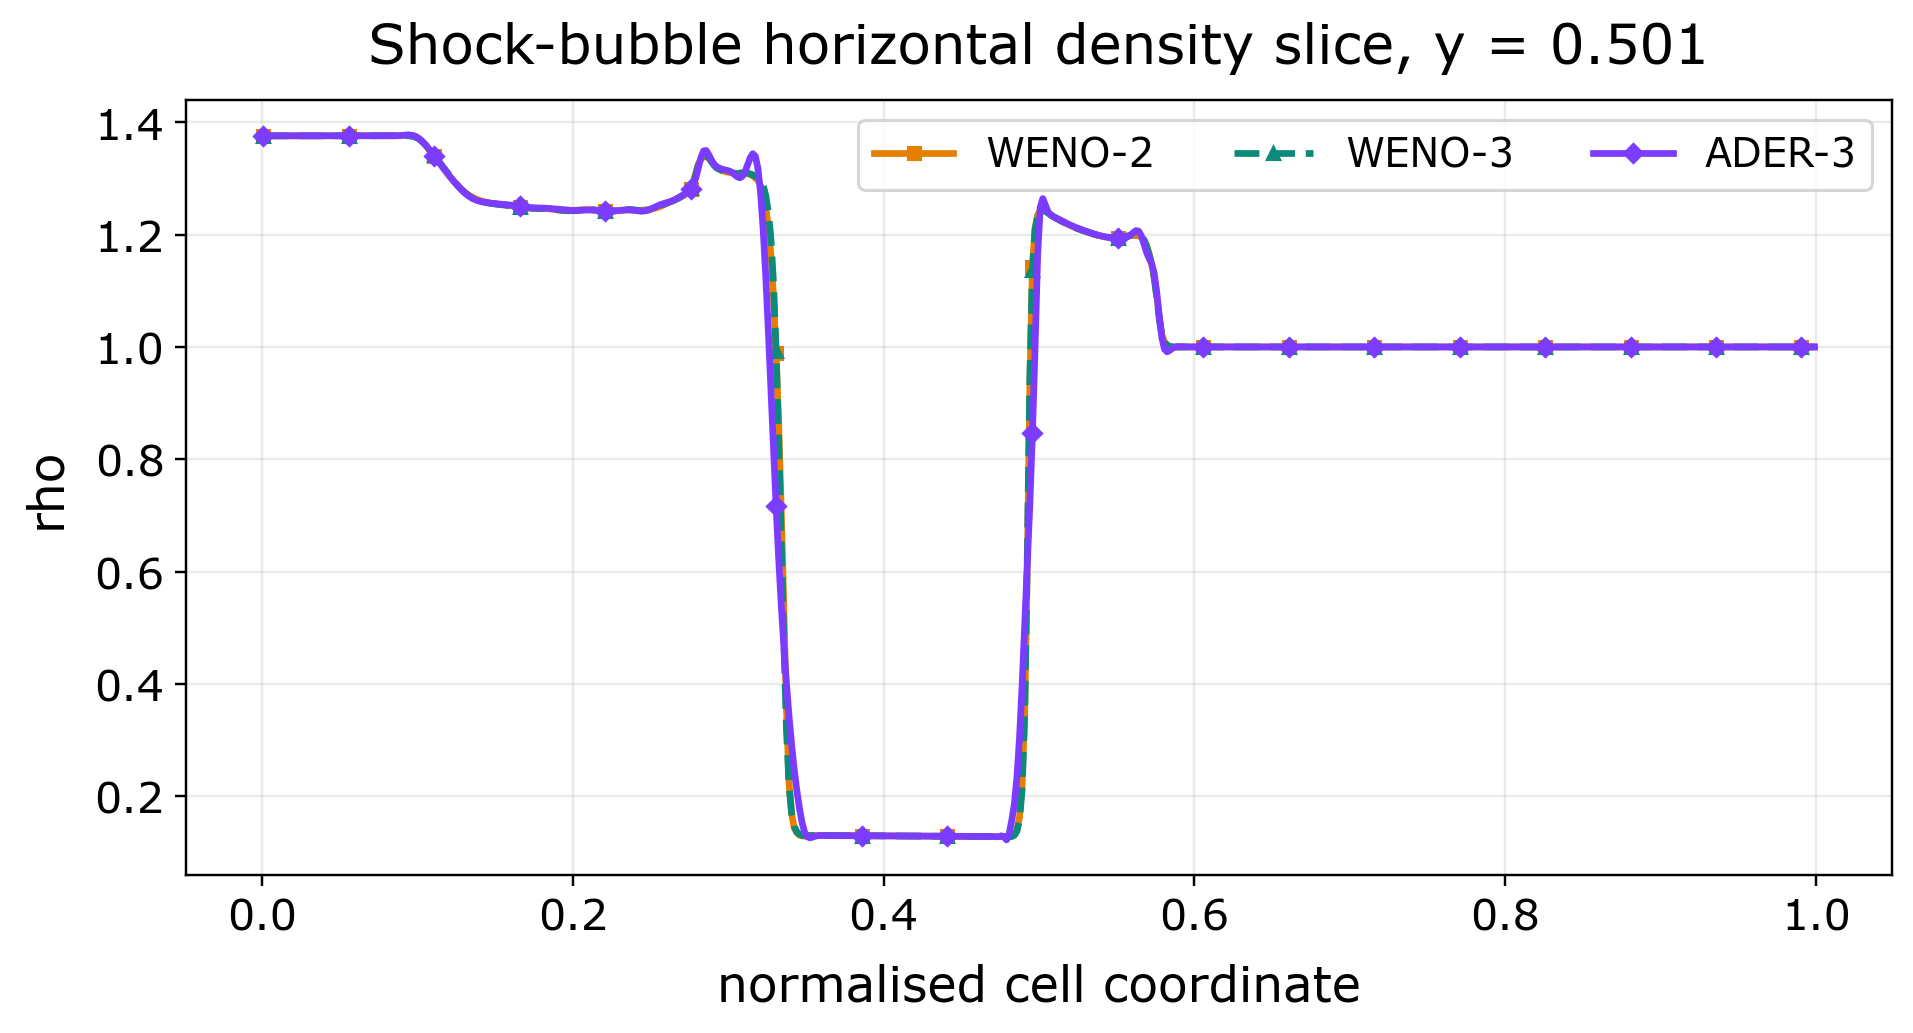
\includegraphics[width=0.90\textwidth]{shock_bubble_slice_hllc_n600.png}
\caption{Shock--bubble density along \(y=0.501\). All cell values contribute to each
line, while markers are thinned for readability.}
\label{fig:shock-slice-discontinuous}
\end{figure}

The three profiles agree through the post-shock and undisturbed states. WENO-2 gives the
broadest bubble boundaries, WENO-3 retains thinner transitions, and ADER-3 produces the
strongest local contrast. Its less smooth edge is confined to the curved interface, where
the Cartesian representation and troubled-interface fallback are most active. It is not
a global background-state error. Figure~\ref{fig:third-order-shock-difference} then tests
whether backend discrepancies alter this resolved flow or remain local.

The WENO-3 map has a visibly layered background. Its mean energy difference is
approximately \(5.2\times10^{-14}\) in the post-shock region on the left and
\(2.7\times10^{-15}\) in the undisturbed right region. These layers follow states of
different magnitude and accumulated arithmetic, while the complete map remains at
roundoff scale with a maximum of \(7.860\times10^{-14}\).

\begin{figure}[!htbp]
\centering
\begin{subfigure}[t]{0.47\textwidth}
\centering
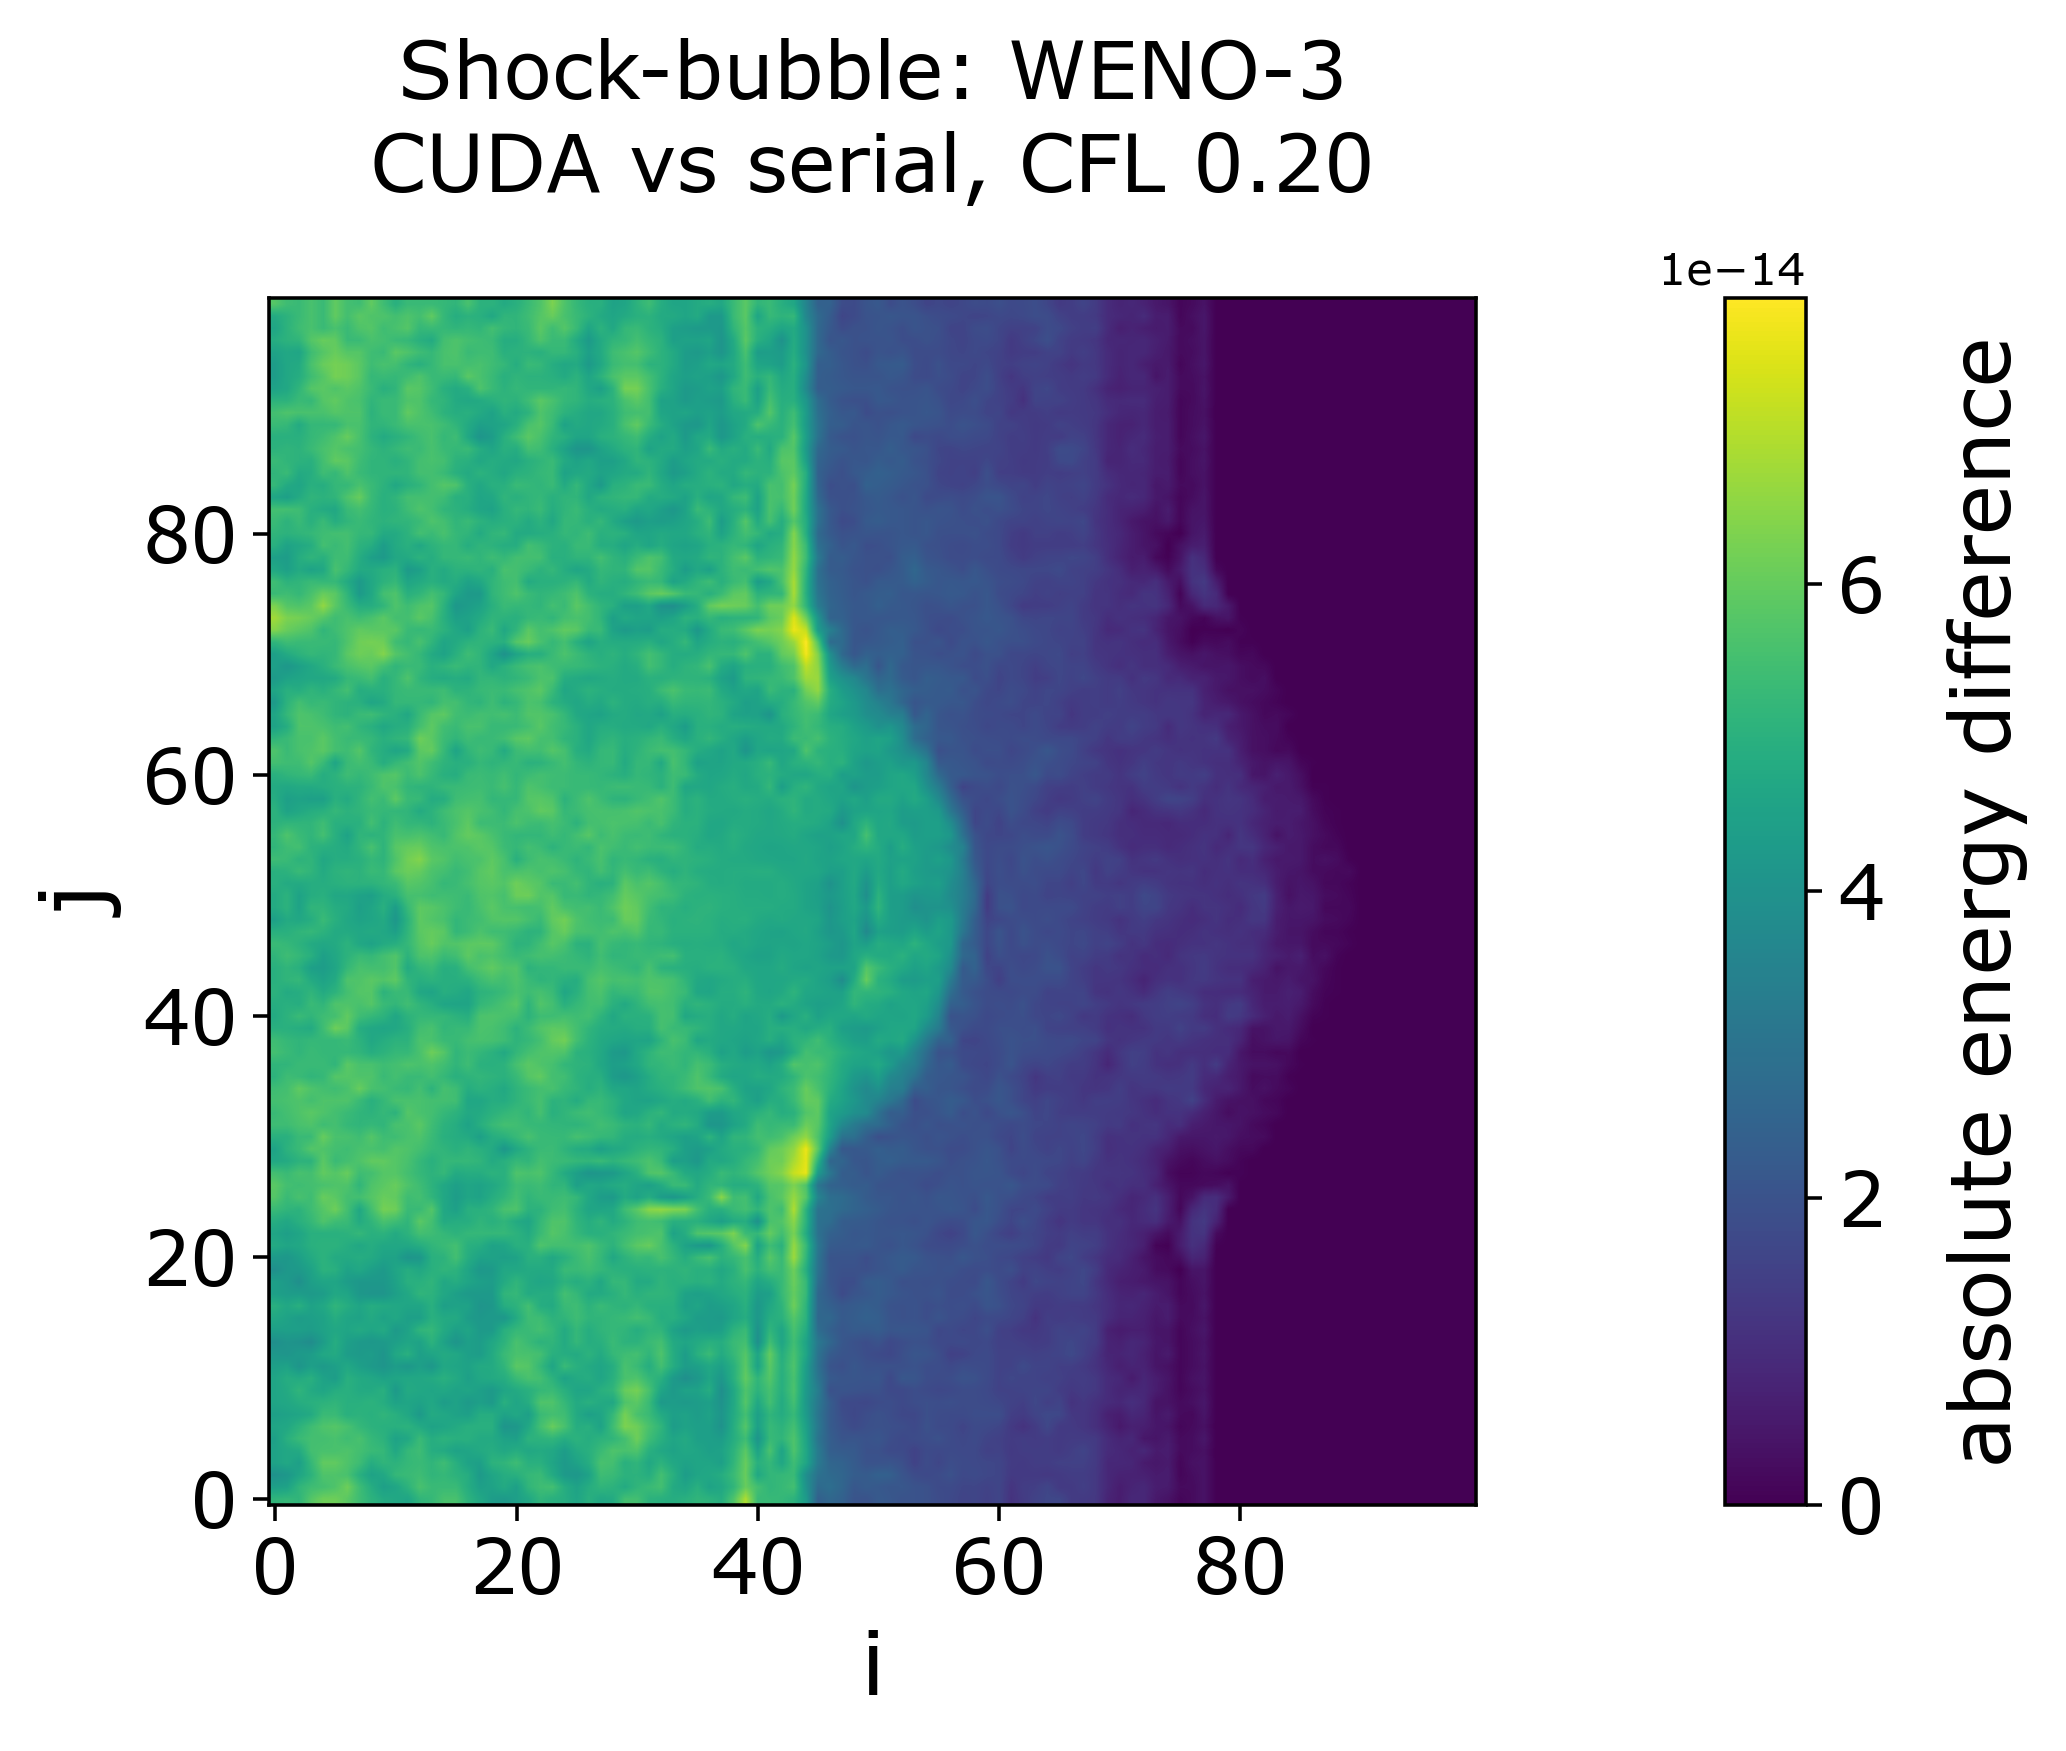
\includegraphics[width=\linewidth]{shock_bubble_weno3_energy_absdiff_cfl020.png}
\caption{WENO-3, CFL 0.20: $\max|\Delta E|=7.860\times10^{-14}$.}
\end{subfigure}\hfill
\begin{subfigure}[t]{0.47\textwidth}
\centering
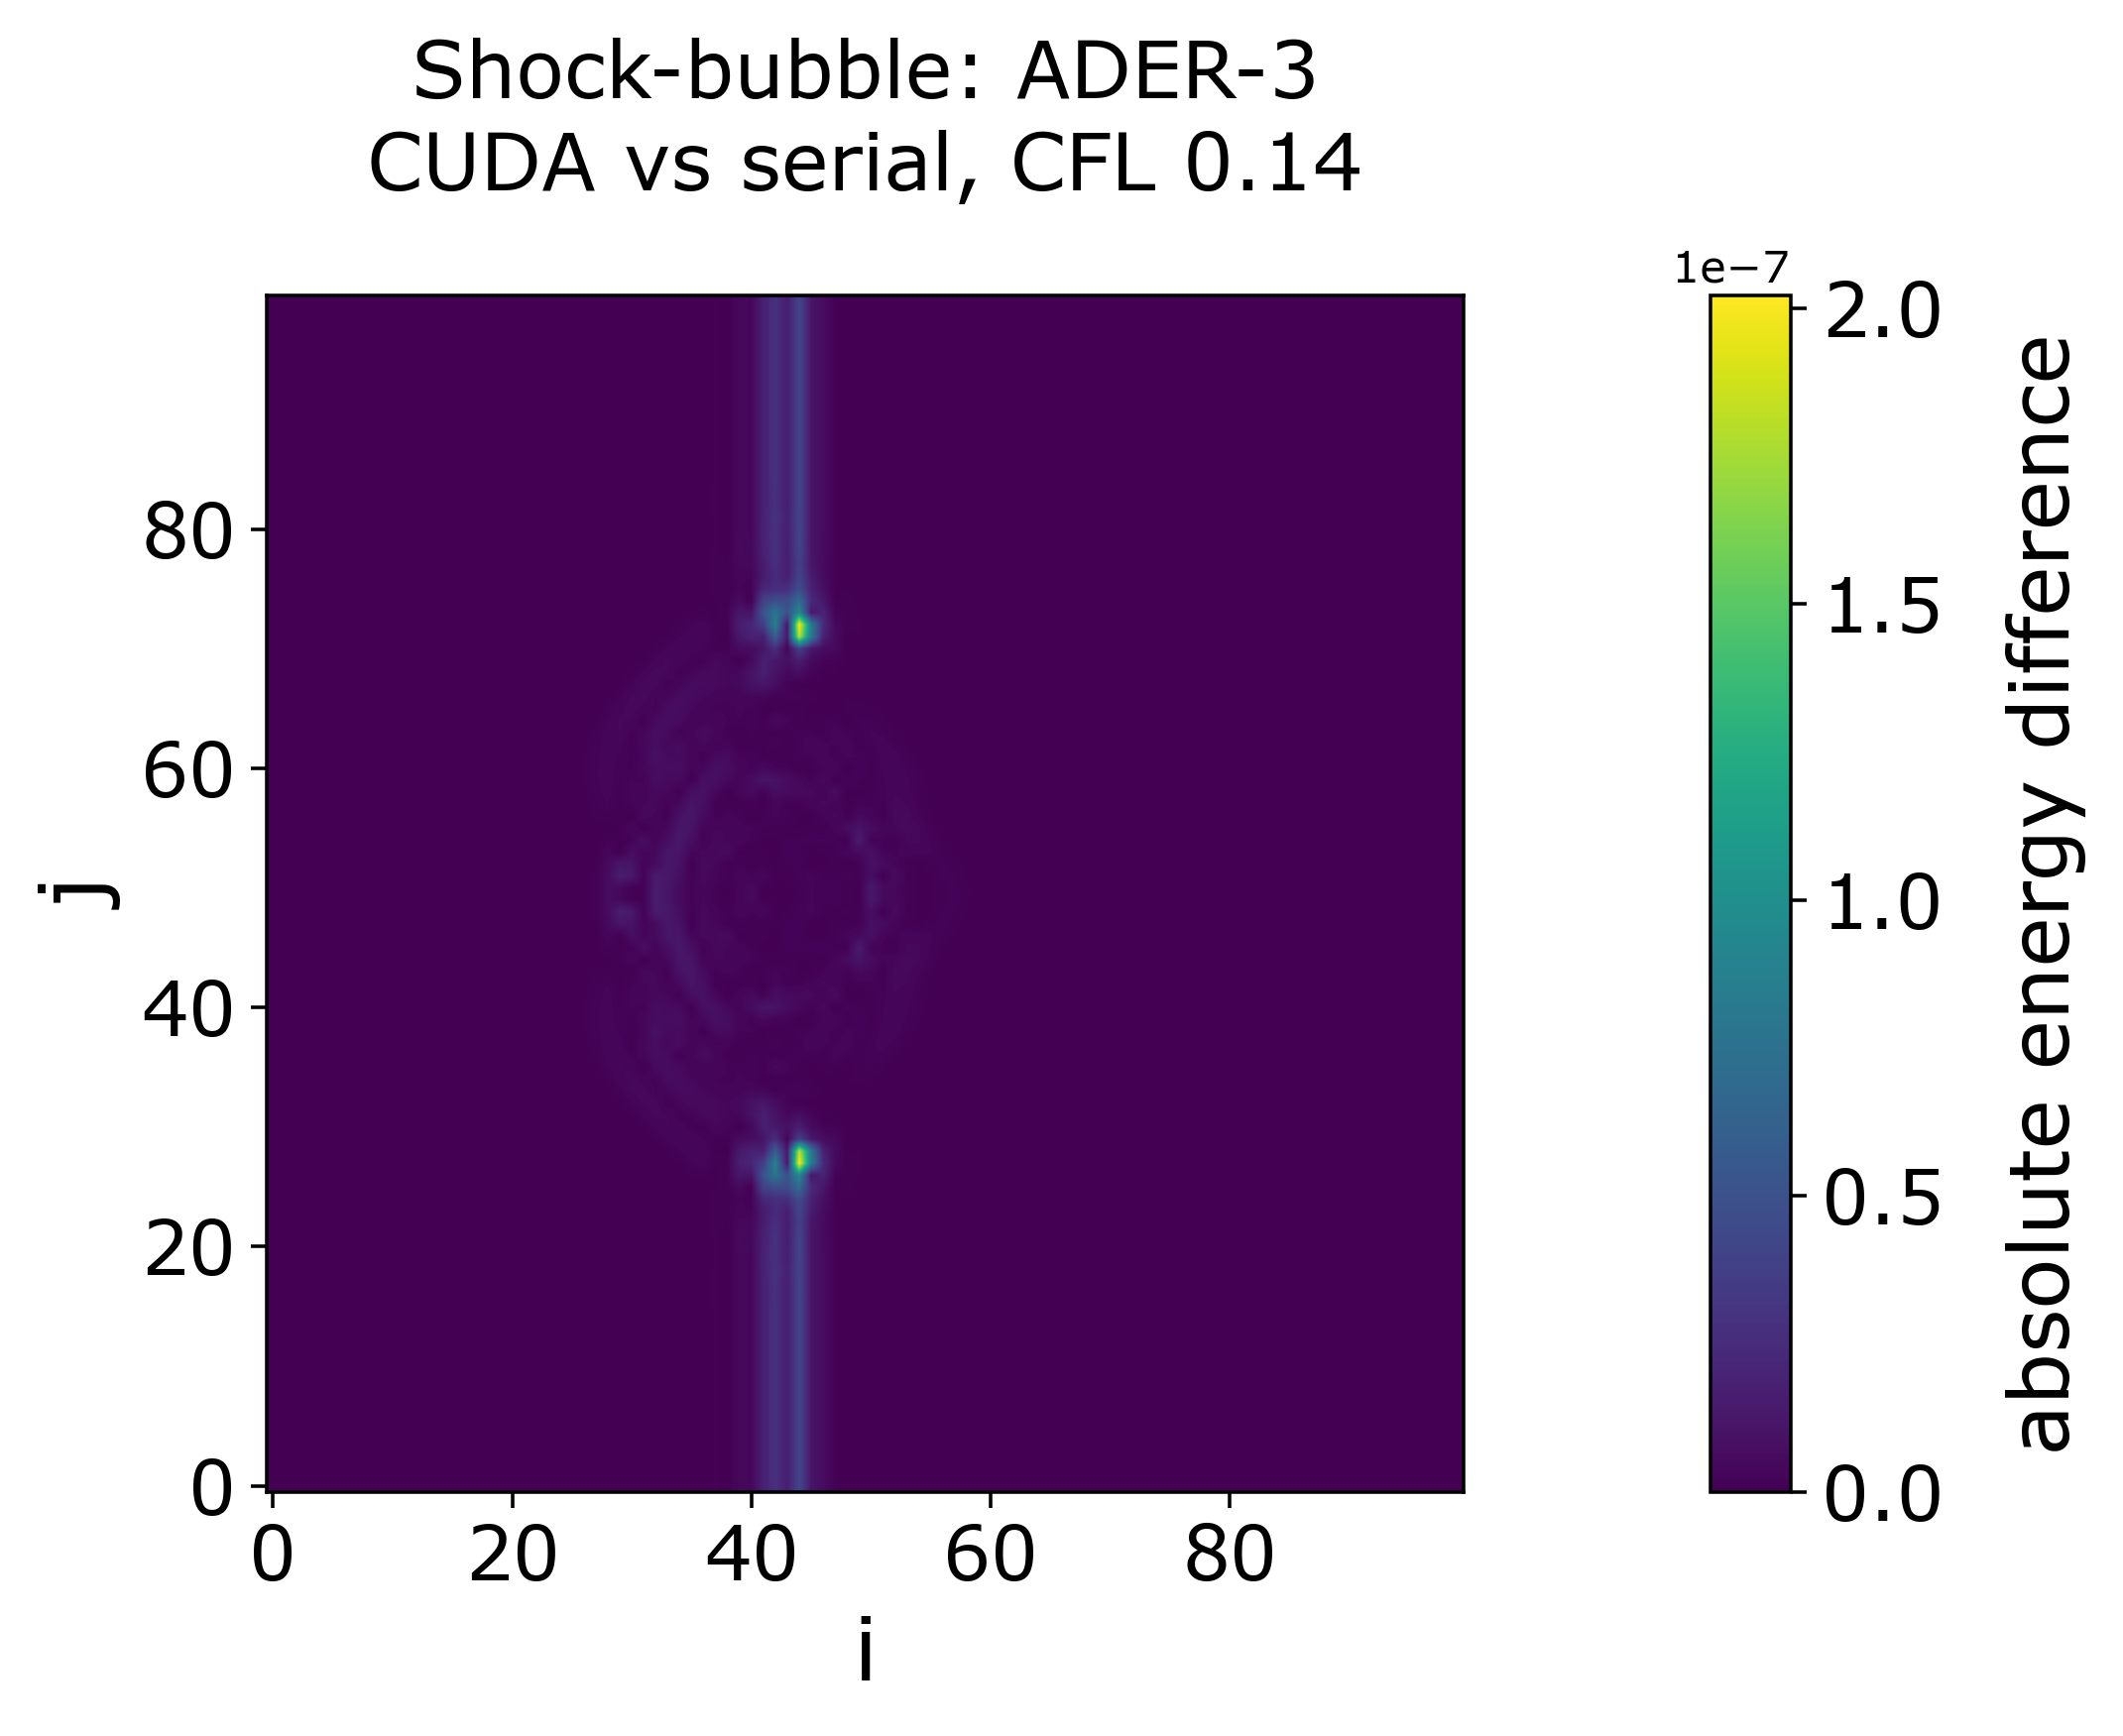
\includegraphics[width=\linewidth]{shock_bubble_ader3_energy_absdiff_cfl014.png}
\caption{ADER-3, CFL 0.14: $\max|\Delta E|=2.021\times10^{-7}$.}
\end{subfigure}
\caption{Absolute CUDA--serial energy differences for the shock--bubble problem at
\(100\times100\). WENO-3 shows broad state-dependent layers at roundoff scale, whereas
ADER-3 is dominated by local peaks where the moving front meets the bubble boundary.
Each panel uses its own colour scale.}
\label{fig:third-order-shock-difference}
\end{figure}

ADER-3 has a more localised signature. Its darker background is interrupted along the
moving shock/contact structure and the faint curved bubble interface. The two strongest
peaks occur near \((i,j)=(44,27)\) and \((44,72)\), where the front intersects the lower
and upper bubble boundaries, and reach \(2.021\times10^{-7}\). They are consistent with
the troubled-interface and fallback sensitivity discussed below, not with displacement of
the complete bubble or shock.

\begin{table}[H]
\centering
\small
\begin{tabular}{llrl}
\toprule
Problem & Method & CUDA maximum difference & Dominant field \\
\midrule
Gaussian advection & WENO-2 & \(3.997\times10^{-15}\) & \(E\) \\
Gaussian advection & WENO-3 & \(8.438\times10^{-15}\) & \(E\) \\
Gaussian advection & ADER-3 & \(2.445\times10^{-12}\) & \(E\) \\
Quadrant Riemann & WENO-2 & \(1.310\times10^{-14}\) & \(v\) \\
Quadrant Riemann & WENO-3 & \(8.527\times10^{-14}\) & \(E\) \\
Quadrant Riemann & ADER-3 & \(3.679\times10^{-12}\) & \(u\) \\
Shock--bubble & WENO-2 & \(1.865\times10^{-14}\) & \(E\) \\
Shock--bubble & WENO-3 & \(7.860\times10^{-14}\) & \(E\) \\
Shock--bubble & ADER-3 & \(2.021\times10^{-7}\) & \(E\) \\
\bottomrule
\end{tabular}
\caption{Maximum absolute field difference against serial at \(100\times100\). OpenMP differences are zero in every exported field.}
\label{tab:backend-diff}
\end{table}

\begin{figure}[!htbp]
\centering
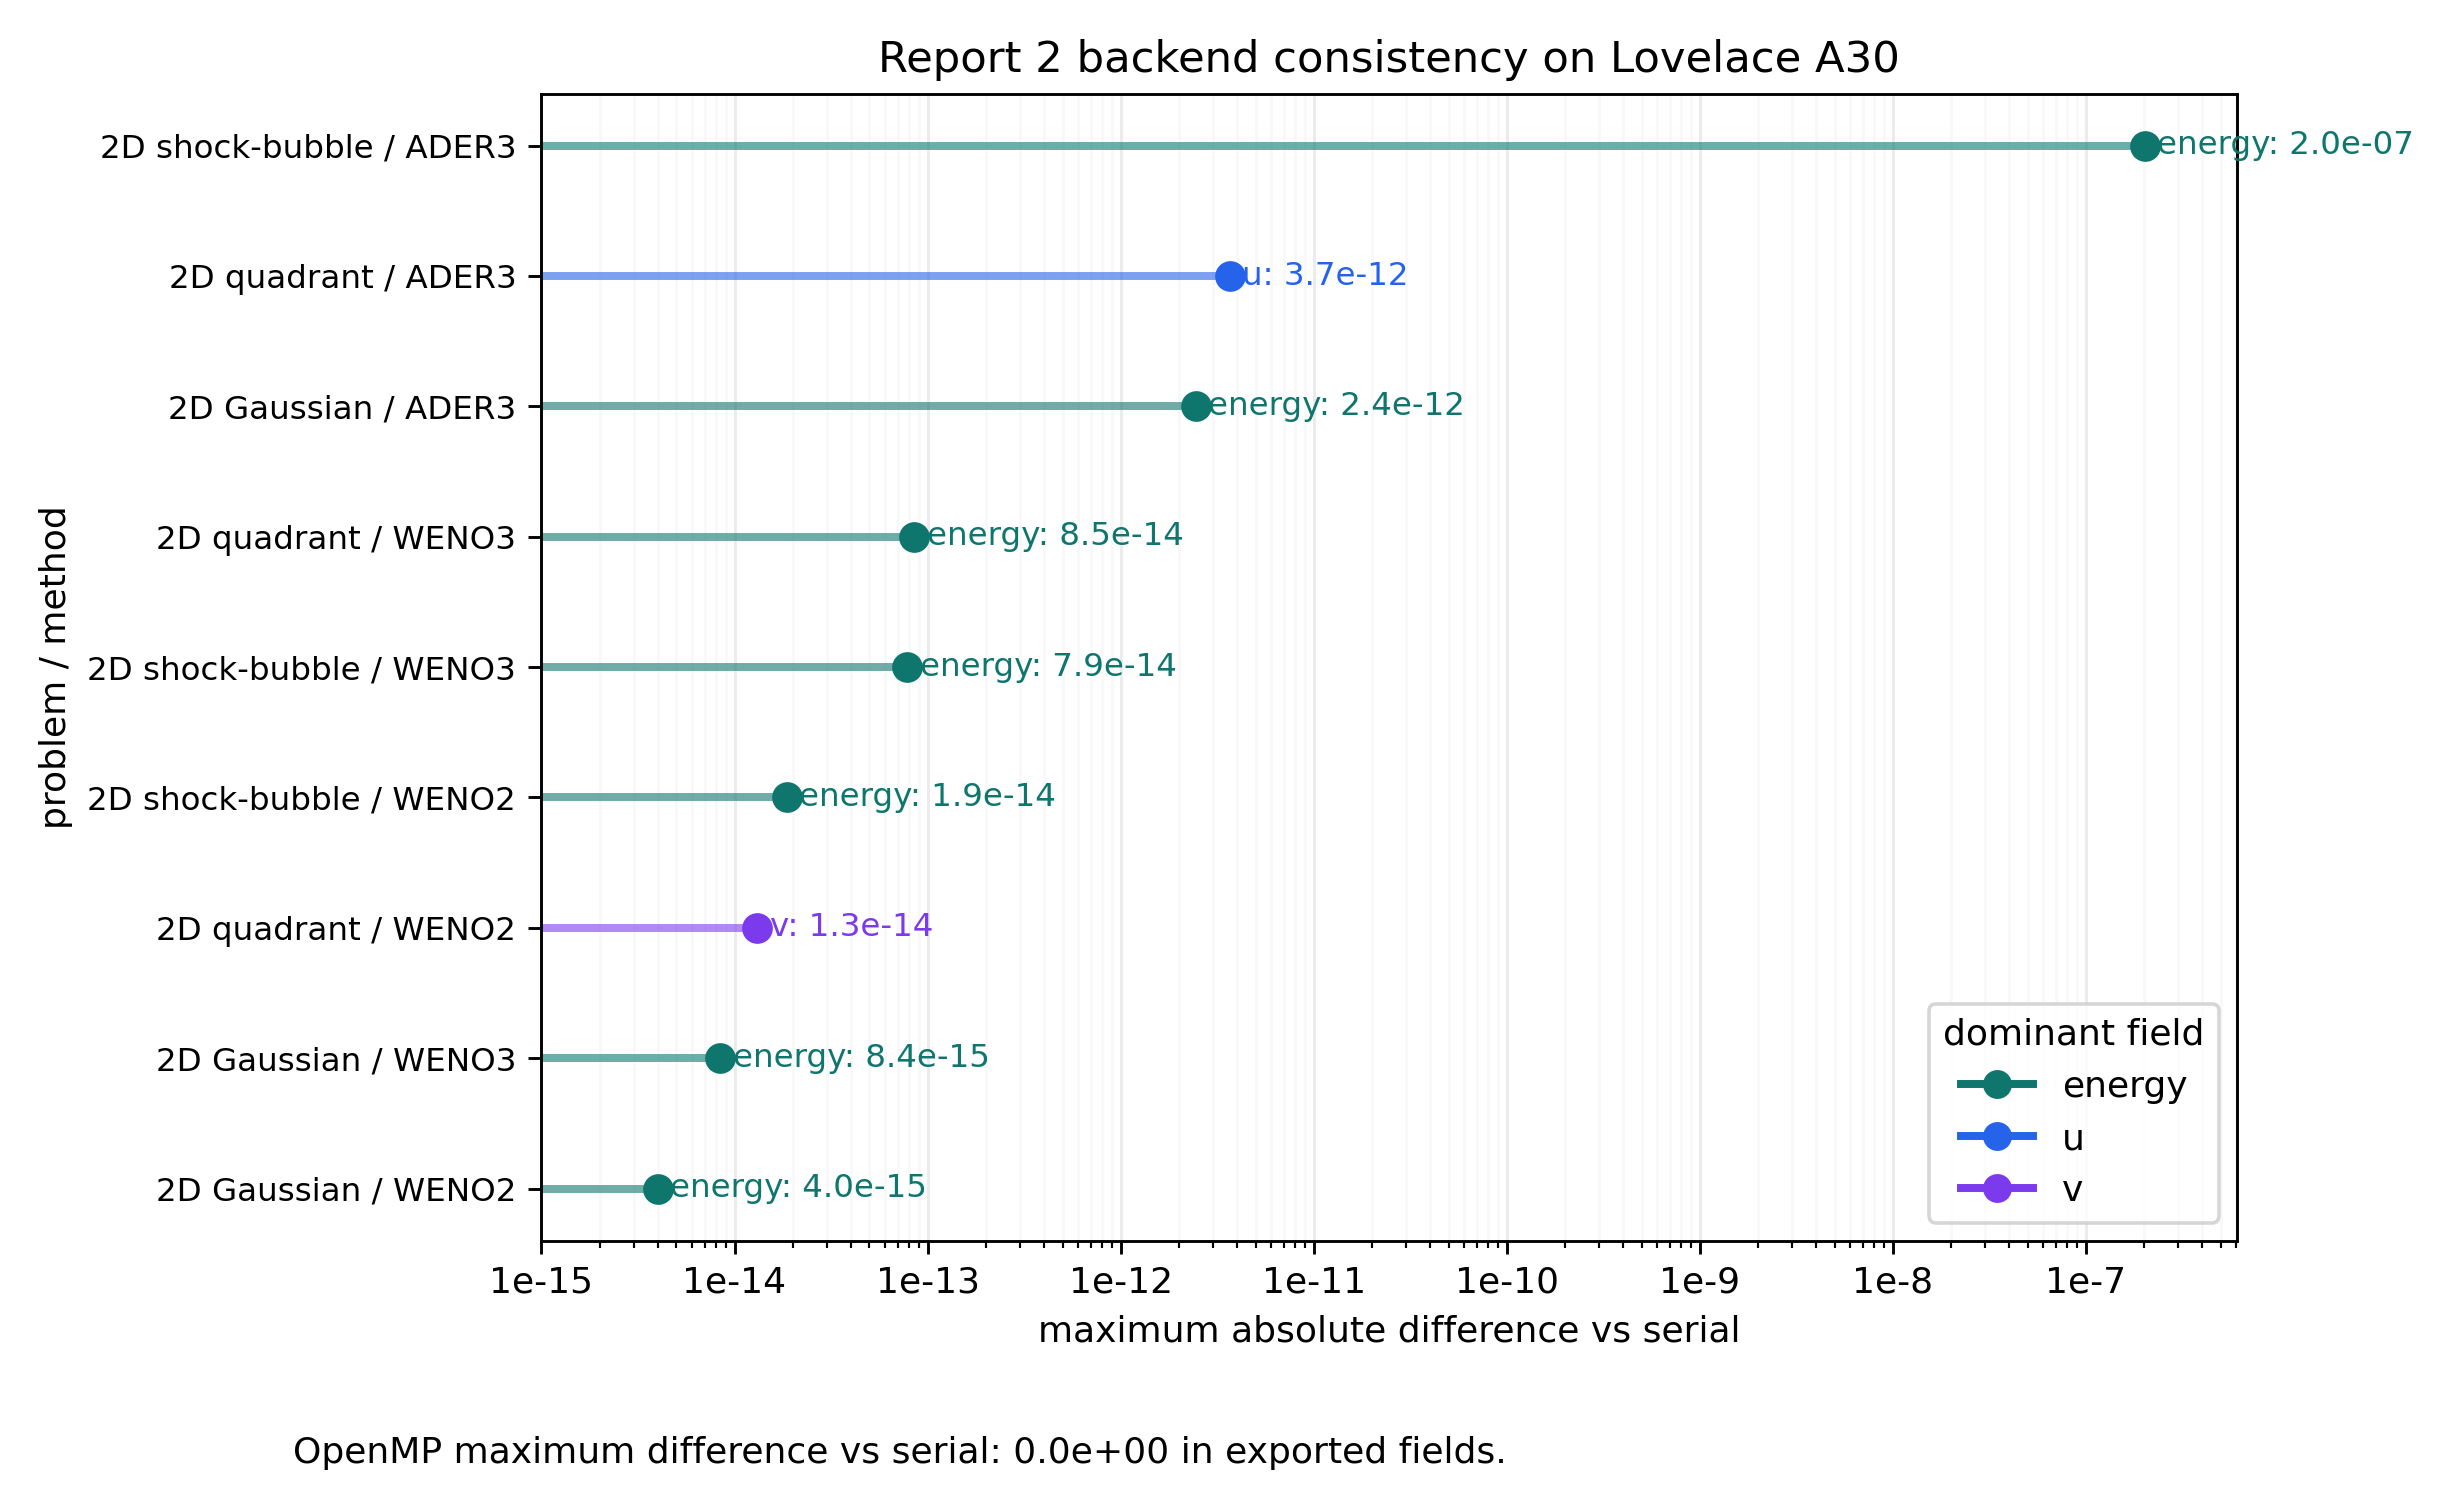
\includegraphics[width=0.88\textwidth]{backend_consistency_max_delta.png}
\caption{Largest CUDA--serial difference for each problem/method pair. OpenMP is omitted from the logarithmic axis because all stored OpenMP--serial differences are exactly zero.}
\label{fig:backend-consistency}
\end{figure}

\FloatBarrier
\section{Backend agreement and admissibility}

OpenMP matches serial exactly in all 45 stored fields. CUDA remains near roundoff for
both WENO methods and below \(4\times10^{-12}\) for smooth and quadrant ADER-3, far below
the discretisation errors in Chapter~\ref{chap:validation}. The sole larger entry is the
local shock--bubble ADER-3 energy difference of \(2.021\times10^{-7}\). Its alignment with
the moving interfaces identifies the nonlinear sensor/fallback branch as the cause rather
than a failed HLLC flux or displaced solution.

Table~\ref{tab:highres-positivity} provides the independent \(600^2\) admissibility check.
Every accepted field remains strictly positive. ADER-3 reaches the lowest shock--bubble
values but remains inside the physical domain.

\begin{table}[H]
\centering
\small
\begin{tabular}{llrr}
\toprule
Problem & Method & \(\min\rho\) & \(\min p\) \\
\midrule
Quadrant Riemann & WENO-2 & 0.137955 & 0.028944 \\
Quadrant Riemann & WENO-3 & 0.137936 & 0.028918 \\
Quadrant Riemann & ADER-3 & 0.137891 & 0.028987 \\
Shock--bubble & WENO-2 & 0.126797 & 0.999112 \\
Shock--bubble & WENO-3 & 0.127368 & 0.999683 \\
Shock--bubble & ADER-3 & 0.122012 & 0.968668 \\
\bottomrule
\end{tabular}
\caption{Minimum density and pressure in the accepted \(600\times600\) discontinuous HLLC fields.}
\label{tab:highres-positivity}
\end{table}

The three implementations therefore produce the same accepted physical solutions. The
following timings compare their execution cost rather than different numerical outcomes.

\FloatBarrier

\chapter{Accuracy and computational performance}
\label{chap:performance}

The preceding chapters established the formal order of accuracy, the admissibility of the
discontinuous solutions, and agreement between the three implementations.  This chapter
asks the practical question that motivates Report~2: how much accuracy is obtained for a
given computational cost, and which hardware is best suited to each method?  HLLC is the
authoritative flux throughout the main analysis.  The earlier HLL route is retained only in
a controlled comparison where problem, grid, CFL number, final time, method, and backend
match.

The high-resolution Gaussian fields in Figure~\ref{fig:gaussian-fields-performance}
provide the physical starting point for this analysis. At \(600\times600\), all three HLLC
methods transport the pulse to the same location and preserve a smooth, symmetric field,
while WENO-3 and ADER-3 retain a slightly more compact peak than WENO-2. The remainder
of this chapter quantifies whether that visual improvement justifies the additional
computational cost.

\section{Measurement procedure}

The main smooth campaign uses the periodic two-dimensional Gaussian problem at
\(t=0.1\) and resolutions \(n=25,50,100,200,600\).  WENO-2 and WENO-3 use
\(\mathrm{CFL}=0.4\), while ADER-3 uses its stable smooth value
\(\mathrm{CFL}=0.25\).  OpenMP uses 16 threads.  Each normal campaign point contains a
warm-up followed by repeated measurements. The best repeat is reported because it is least
affected by unrelated activity on the shared Lovelace node.  The speedup of backend \(b\)
is
\begin{equation}
  S_b = \frac{T_{\mathrm{serial}}}{T_b},
  \qquad
  E_{\mathrm{OMP}}(p)=\frac{S_{\mathrm{OMP}}(p)}{p},
  \label{eq:speedup-efficiency}
\end{equation}
Here \(T_{\mathrm{serial}}\) is the serial runtime, \(T_b\) is the runtime of
backend \(b\), and \(S_b\) is that backend's speedup relative to serial.
For OpenMP, \(p\) is the thread count, \(S_{\mathrm{OMP}}(p)\) is the speedup
measured with those \(p\) threads, and \(E_{\mathrm{OMP}}(p)\) is the resulting
parallel efficiency. Thus \(E_{\mathrm{OMP}}=1\) denotes ideal linear scaling.

These method-specific CFL values make the cross-method runtime an end-to-end efficiency
measurement rather than a fixed-time-step kernel benchmark.  In other words, the measured
cost includes the number of updates required by each method in its validated stable
configuration.  Backend speedups remain strictly controlled because all backends use the
same CFL and accepted step count for a given method.  The HLL--HLLC comparison later in
this chapter is stricter still: only rows with matching method, problem, backend, grid,
CFL, final time, and accepted step count are compared.  Consequently, different CFL
numbers are never used to create a favourable backend or flux comparison.

All performance commands use \texttt{--output=none}. Writing the full field to CSV is
therefore excluded.  The outer Python driver times the complete solver process, so the
measurement still contains executable start-up, initialization, the time integration,
terminal diagnostics, and one final error-norm pass for the smooth Gaussian problem.  The
last two costs are small compared with hundreds or thousands of updates at large \(n\), but
they correctly remain visible at the smallest grids.  Accuracy is measured from the same
run using
\begin{equation}
  L_1(\rho)=\frac{1}{N}\sum_{i=1}^{N}
       \left|\rho_i-\rho_i^{\mathrm{exact}}\right|,
  \label{eq:performance-l1}
\end{equation}
where \(N\) is the total number of cells, \(i\) indexes a cell, and
\(\rho_i^{\mathrm{exact}}\) is its exact finite-volume density average. The
corresponding \(L_2\) and \(L_\infty\) norms are retained in the processed data.

The discontinuous campaign uses the quadrant Riemann and shock--bubble problems at
\(t=0.2\), with field output again disabled.  Its main grid sequence is
\(n=50,100,200,600\).  These cases have no smooth exact solution, so their performance is
reported separately from the Gaussian error--runtime comparison.

\section{Smooth accuracy--cost landscape}

Figure~\ref{fig:smooth-runtime-performance} shows the first important change of regime.
At small grids CUDA pays an approximately fixed cost for process and device setup, kernel
launches, and synchronization \cite{nvidia129}, so it is not automatically the fastest backend.  Serial and
OpenMP costs rise much more rapidly with resolution, while the CUDA curves remain shallow
until the device has enough work to amortise those fixed costs.  This is particularly clear
for WENO-2, whose inexpensive spatial operator gives the GPU less arithmetic with which to
hide overhead. The balance between arithmetic work and memory traffic is the central idea of
the roofline performance model \cite{williams2009}.

\begin{figure}[H]
\centering
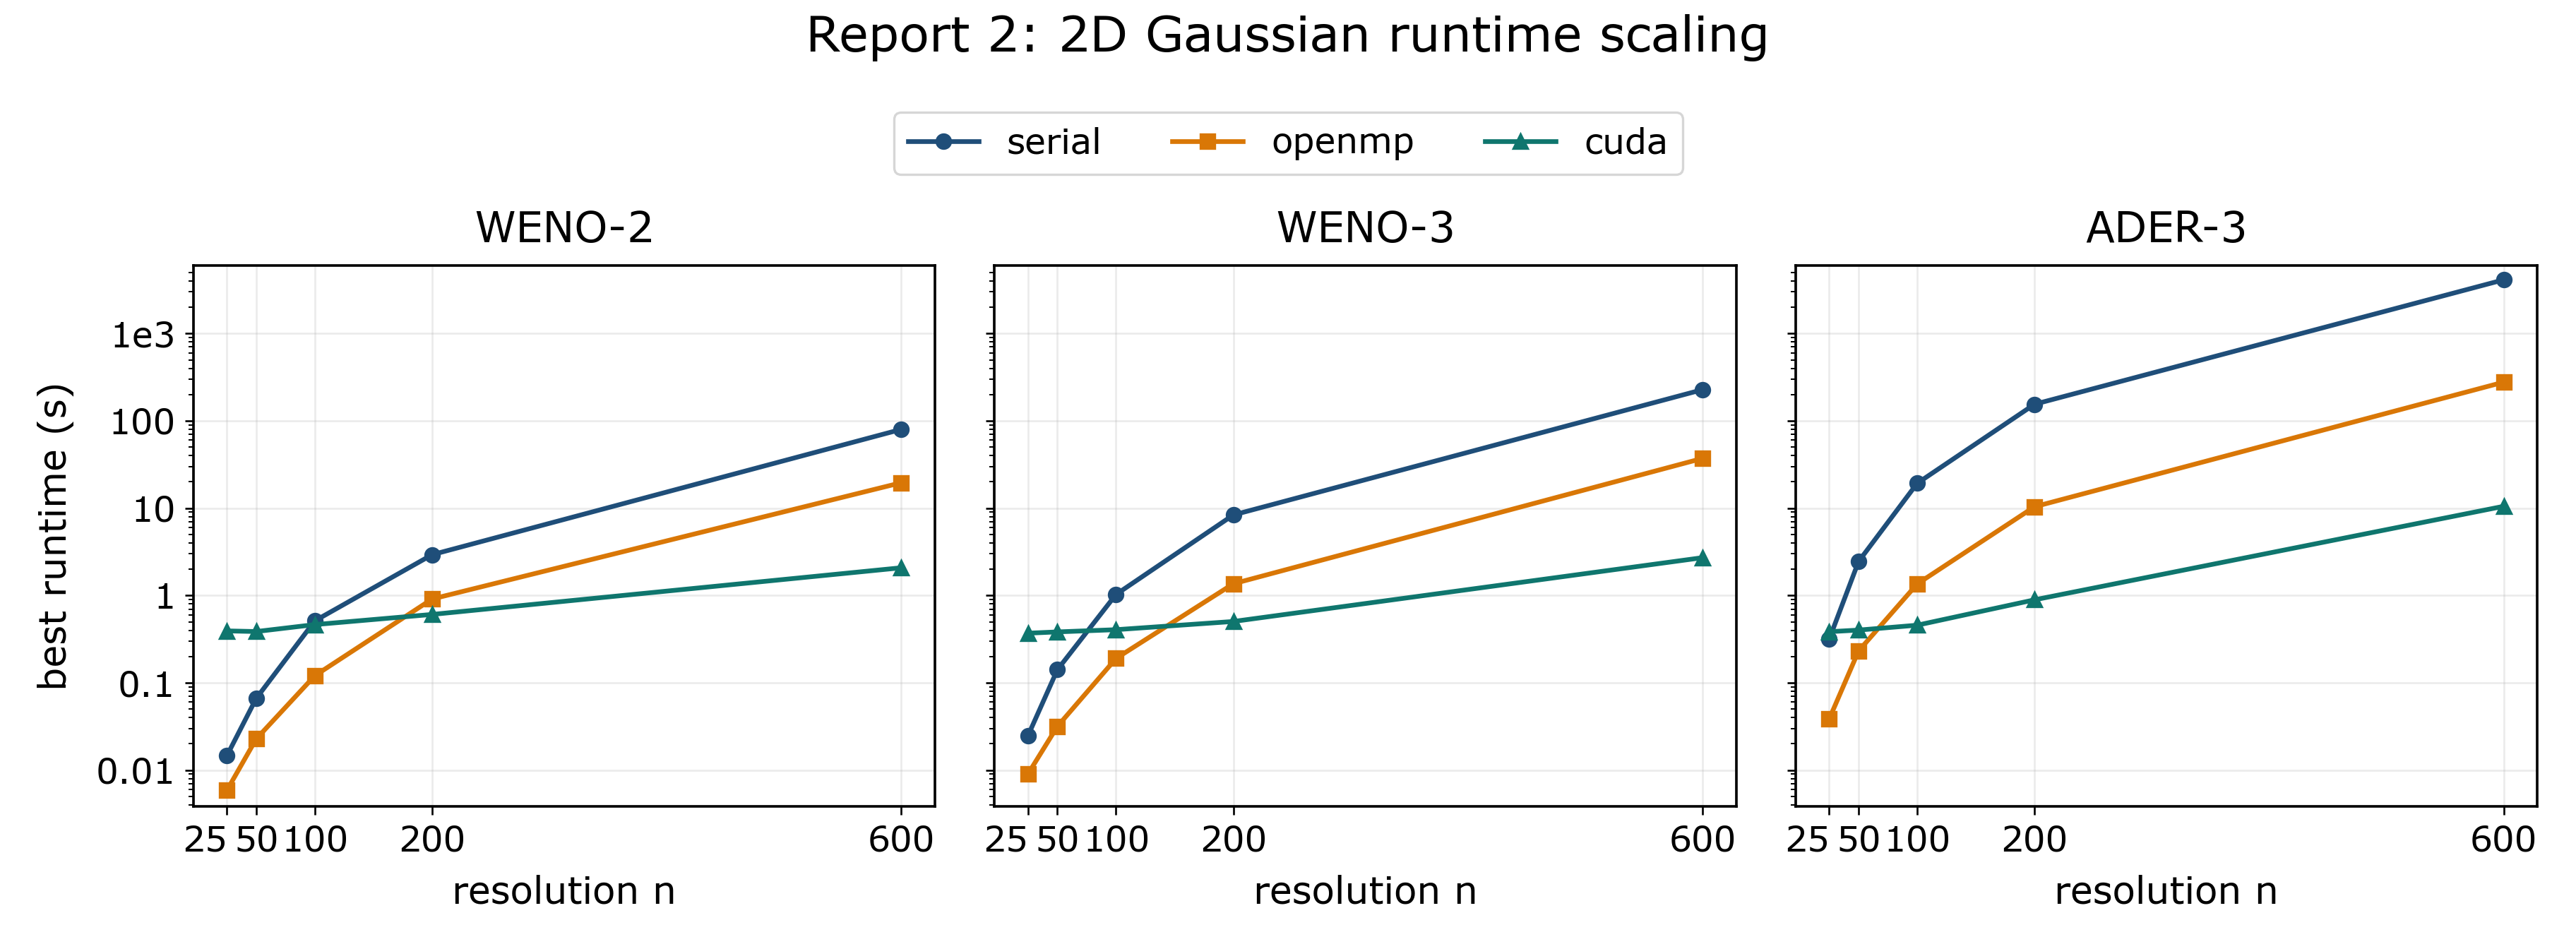
\includegraphics[width=0.98\textwidth]{performance_smooth_runtime_hllc.png}
\caption{HLLC runtime scaling for the smooth two-dimensional Gaussian problem at
\(n=25,50,100,200,600\).  OpenMP uses 16 threads, and field output is disabled during
timing.}
\label{fig:smooth-runtime-performance}
\end{figure}

The same data expressed as speedup are shown in
Figure~\ref{fig:smooth-speedup-performance}.  OpenMP provides a useful but bounded gain:
at \(600^2\) it reaches \(4.08\), \(6.12\), and \(14.86\) for WENO-2, WENO-3, and
ADER-3.  CUDA benefits much more strongly from increasing method complexity, reaching
\(38.43\), \(83.84\), and \(392.01\), respectively.  These numbers do not imply that
ADER-3 is the fastest method.  They show that its much larger serial workload contains
more parallel work and is therefore reduced by a larger factor.

\begin{figure}[H]
\centering
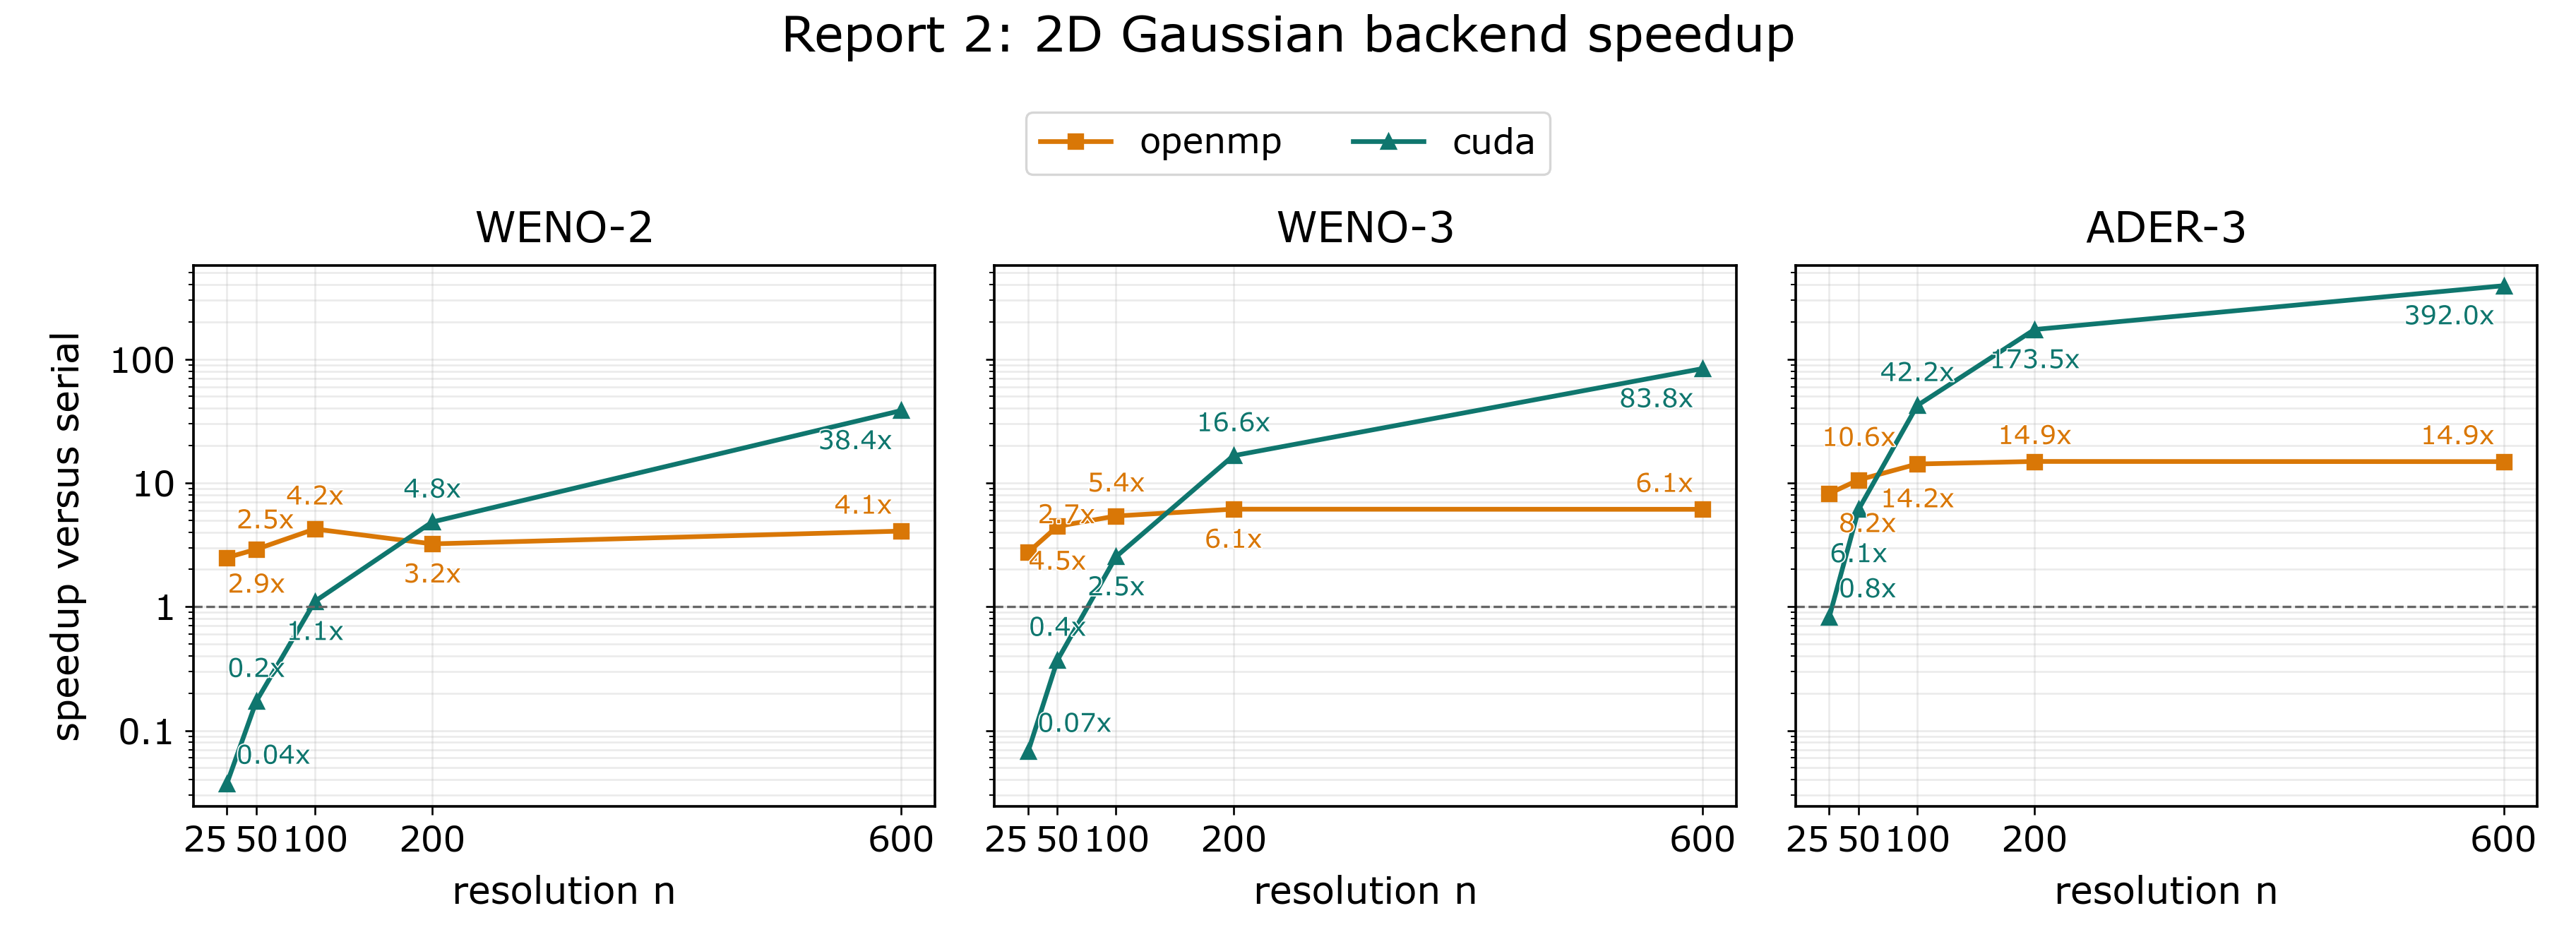
\includegraphics[width=0.98\textwidth]{performance_smooth_speedup_hllc.png}
\caption{HLLC backend speedup relative to serial for the smooth Gaussian campaign at
\(n=25,50,100,200,600\).  OpenMP uses 16 threads.}
\label{fig:smooth-speedup-performance}
\end{figure}

Table~\ref{tab:smooth-n600-performance} combines cost and accuracy at the largest common
all-backend grid.  WENO-3 and ADER-3 reduce the WENO-2 density error by factors of
approximately 27.2 and 28.0.  On serial CPU this accuracy is expensive: ADER-3 takes more
than \(4.1\times10^3\) seconds.  CUDA changes the ranking.  WENO-3 requires only 2.71 s,
close to the 2.08 s WENO-2 run, while retaining its much lower error.  ADER-3 reaches almost
the same error as WENO-3 but takes 10.51 s.  WENO-3 is therefore the strongest measured
accuracy--runtime compromise at \(600^2\). ADER-3 demonstrates the desired order and large
parallel speedup, but its one-step predictor is not yet cost competitive.

\begin{table}[H]
\centering
\small
\begin{tabular}{lrrrrrr}
\toprule
Method & \(L_1(\rho)\) & Serial & OpenMP & CUDA & OMP sp. & CUDA sp. \\
\midrule
WENO-2 & \(4.703\times10^{-7}\) & 79.86 & 19.56 & 2.08 & 4.08 & 38.43 \\
WENO-3 & \(1.726\times10^{-8}\) & 227.31 & 37.13 & 2.71 & 6.12 & 83.84 \\
ADER-3 & \(1.681\times10^{-8}\) & 4118.48 & 277.20 & 10.51 & 14.86 & 392.01 \\
\bottomrule
\end{tabular}
\caption{Smooth HLLC results at \(600\times600\) on Lovelace A30.  Times are best
repeated wall-clock measurements in seconds.}
\label{tab:smooth-n600-performance}
\end{table}

Figure~\ref{fig:smooth-tradeoff-performance} presents the full grid sequence directly in
accuracy--runtime space.  Moving down means lower error and moving left means lower cost.
The error for a fixed method and resolution is essentially backend independent after the
consistency checks in Chapter~\ref{chap:backend-consistency}. Changing backend therefore
moves a point horizontally.  This is why groups of serial, OpenMP, and CUDA points lie on
the same error level.  CUDA shifts the third-order methods far enough left that their
accuracy advantage becomes practical rather than merely formal.

\begin{figure}[H]
\centering
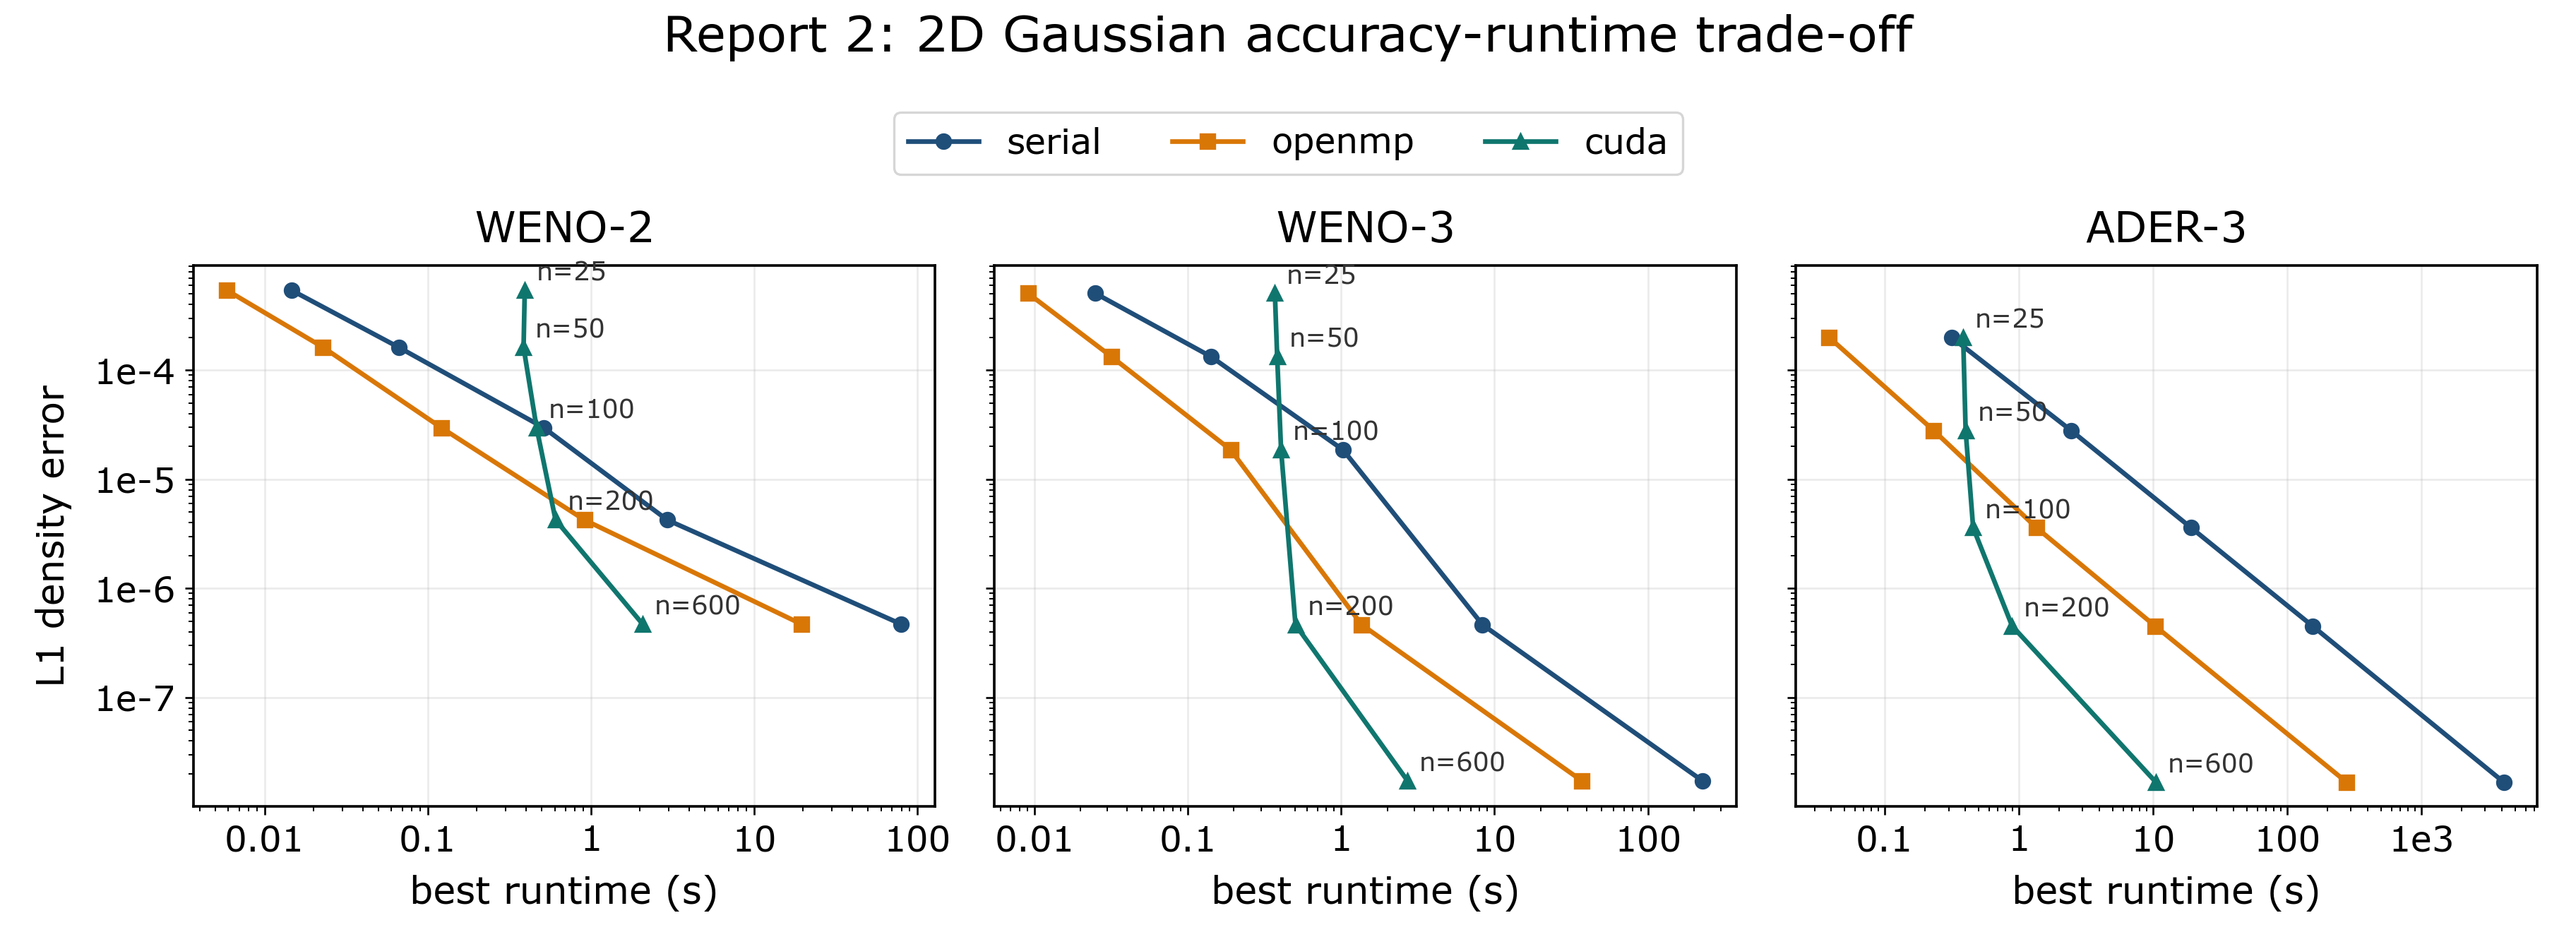
\includegraphics[width=0.96\textwidth]{performance_smooth_accuracy_runtime_hllc.png}
\caption{HLLC density-error versus runtime for the smooth Gaussian campaign.}
\label{fig:smooth-tradeoff-performance}
\end{figure}

The conclusion is not simply that higher order is better.  WENO-2 remains attractive for
small or latency-dominated calculations, where the target error is modest.  WENO-3 becomes
preferable as resolution and accuracy requirements increase.  ADER-3 offers comparable
third-order error but currently requires substantially more work per cell, so its value
depends on whether future kernel and predictor optimization can close that cost gap.

\section{Performance on discontinuous problems}

The two discontinuous cases test whether the smooth conclusions survive when HLLC branch
selection, positivity checks, and local fallback are active.  Table~\ref{tab:discontinuous-n600}
shows the \(600^2\) endpoint.  CUDA remains decisive: speedups range from 48.57 to 478.53
for the quadrant problem and from 84.98 to 427.15 for shock--bubble.  The larger ADER-3
speedups again arise from a very expensive serial baseline, not from a lower absolute cost.
Its CUDA runs remain slower than either WENO method.

\begin{table}[H]
\centering
\small
\begin{tabular}{llrrrrr}
\toprule
Case & Method & Serial & OpenMP & CUDA & OMP sp. & CUDA sp. \\
\midrule
Quadrant & WENO-2 & 388.55 & 95.18 & 8.00 & 4.08 & 48.57 \\
Quadrant & WENO-3 & 1153.71 & 197.29 & 11.86 & 5.85 & 97.24 \\
Quadrant & ADER-3 & 21749.43 & 1941.68 & 45.45 & 11.20 & 478.53 \\
Shock--bubble & WENO-2 & 741.91 & 173.33 & 8.54 & 4.28 & 86.89 \\
Shock--bubble & WENO-3 & 2067.88 & 356.72 & 24.33 & 5.80 & 84.98 \\
Shock--bubble & ADER-3 & 36977.24 & 2496.39 & 86.57 & 14.81 & 427.15 \\
\bottomrule
\end{tabular}
\caption{HLLC discontinuous timing at \(600\times600\).  The selected stable CFL values
are 0.2 for both WENO methods and 0.14 for ADER-3.}
\label{tab:discontinuous-n600}
\end{table}

The absolute CUDA costs qualify these speedups. In the quadrant case, WENO-3 costs
1.48 times WENO-2 and ADER-3 costs 3.83 times WENO-3. The corresponding shock--bubble
ratios are 2.85 and 3.56. WENO-3 therefore buys cleaner contact resolution at a moderate
cost, whereas much of ADER-3's extra predictor work is lost near shocks when the robust
fallback is activated. Its large speedup reflects abundant parallel work, not the lowest
time to solution.

\begin{figure}[H]
\centering
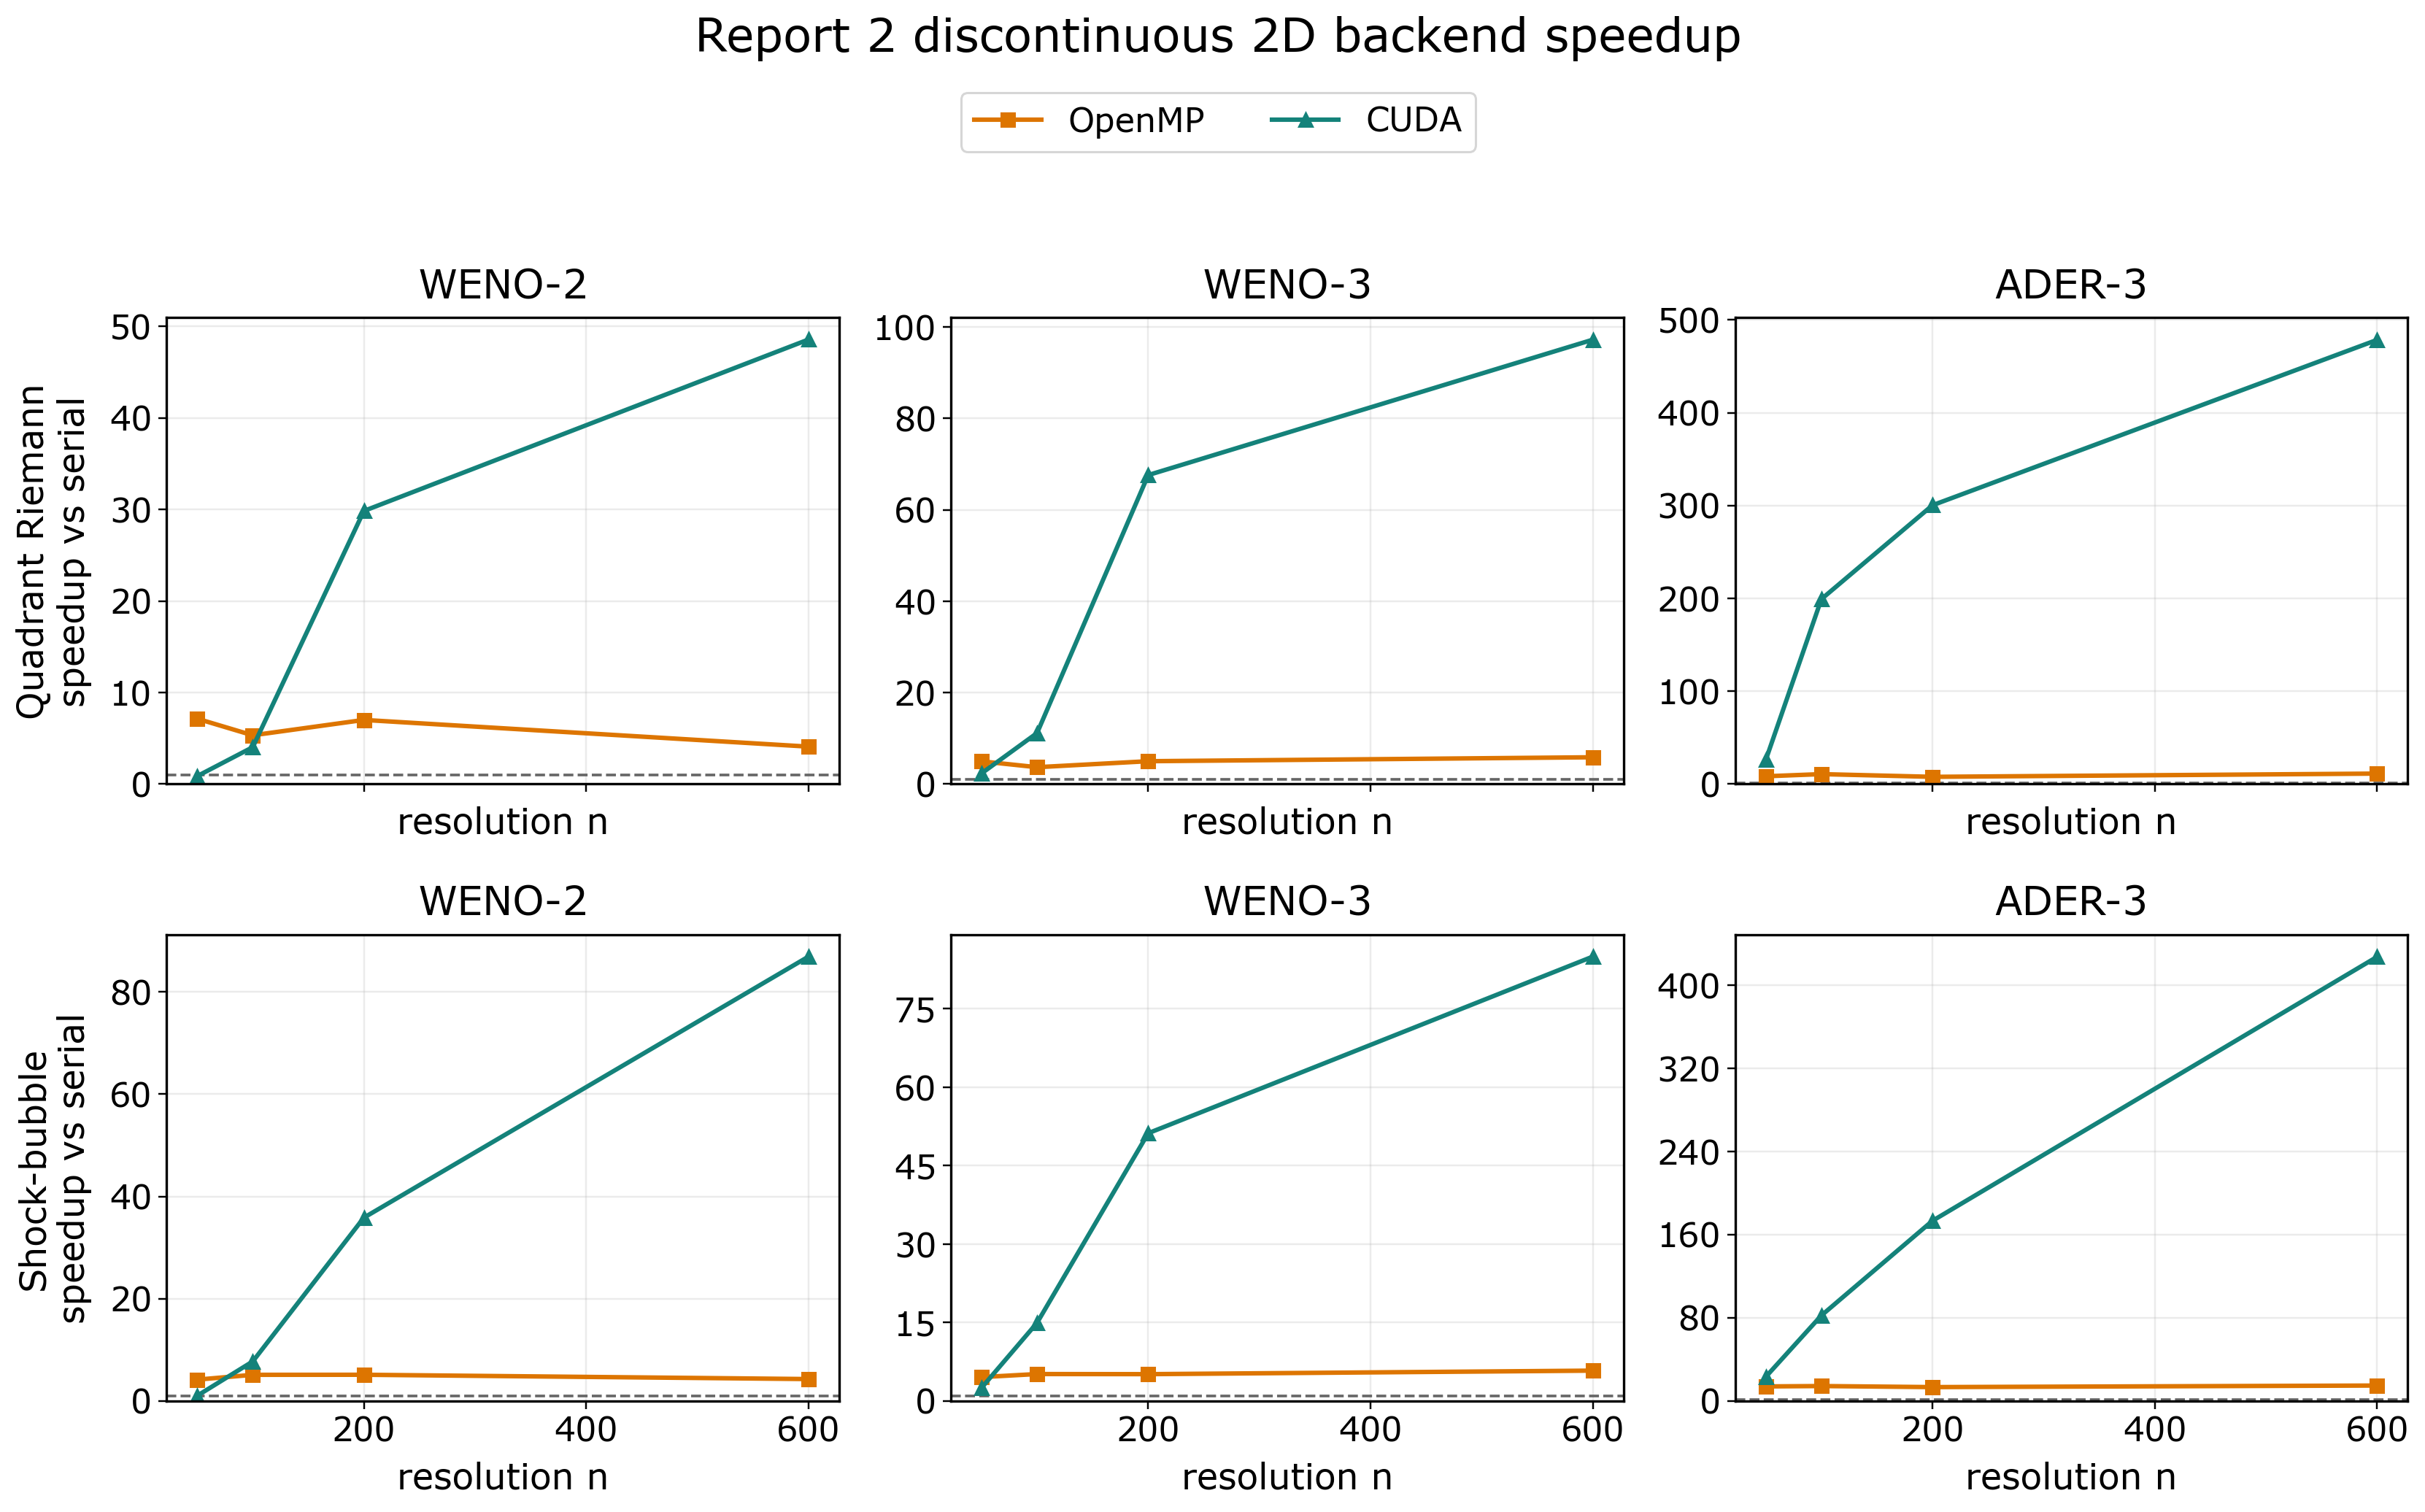
\includegraphics[width=0.94\textwidth]{performance_discontinuous_speedup_hllc.png}
\caption{OpenMP and CUDA speedup for the HLLC discontinuous campaign at
\(n=50,100,200,600\).}
\label{fig:discontinuous-speedup-performance}
\end{figure}

Figure~\ref{fig:discontinuous-speedup-performance} also exposes the crossover behaviour.
CUDA is unattractive at the smallest grids but improves rapidly once the calculation is
large enough.  OpenMP reaches its useful range earlier, then flattens because synchronization,
temporary storage, reductions, and the remaining serial work do not shrink with the same
rate as the cell-local loops.  The shock--bubble ADER-3 CUDA speedup decreases from its
\(n=200\) value to \(n=600\), but remains above 400. The result is better read as evidence
of a changing bottleneck than as a failure of acceleration.

\section{Matched HLL and HLLC comparison}

HLLC is the main Report~2 flux because it restores the contact wave omitted by HLL.  The
older HLL data are nevertheless useful in this chapter: they reveal whether the additional
wave structure changes measured accuracy and cost.  Only strict matches are used here.
The compared rows have the same problem, method, grid, CFL number, final time, backend,
and accepted time-step count, so the flux route is the intended difference.

\begin{table}[H]
\centering
\small
\begin{tabular}{lrrrrr}
\toprule
Method & HLL time & HLLC time & HLL \(L_1\) & HLLC \(L_1\) & Error change \\
\midrule
WENO-2 & 8.51 & 2.08 & \(4.746\times10^{-7}\) & \(4.703\times10^{-7}\) & \(-0.9\%\) \\
WENO-3 & 6.18 & 2.71 & \(5.112\times10^{-8}\) & \(1.726\times10^{-8}\) & \(-66.2\%\) \\
ADER-3 & 10.03 & 10.51 & \(5.063\times10^{-8}\) & \(1.681\times10^{-8}\) & \(-66.8\%\) \\
\bottomrule
\end{tabular}
\caption{Matched smooth CUDA comparison at \(600\times600\).  A negative error change
means that HLLC is more accurate.}
\label{tab:hll-hllc-n600}
\end{table}

\begin{figure}[H]
\centering
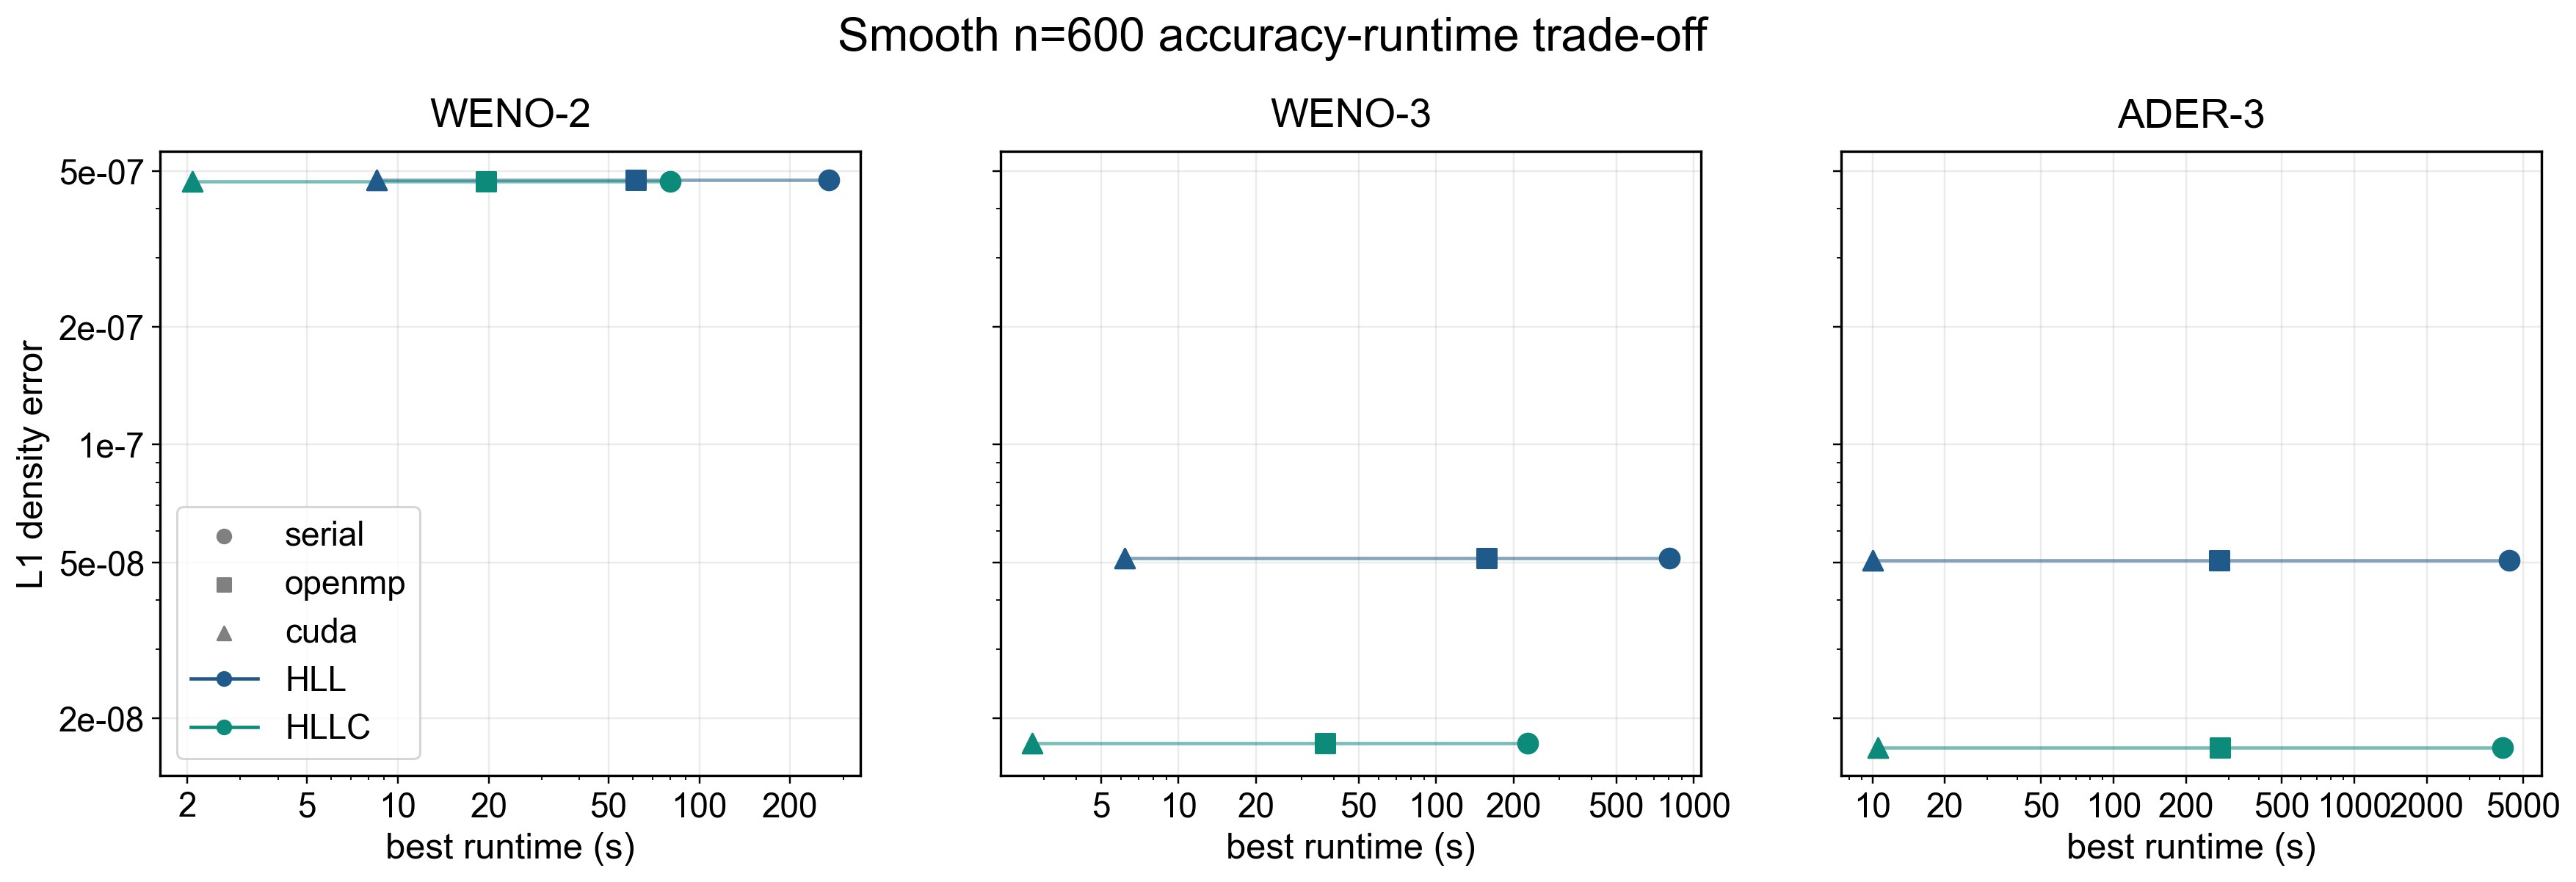
\includegraphics[width=0.96\textwidth]{performance_hll_hllc_n600_tradeoff.png}
\caption{Matched HLL--HLLC accuracy--runtime comparison at \(600\times600\).  Marker
shape identifies backend and colour identifies flux route.}
\label{fig:hll-hllc-n600-tradeoff}
\end{figure}

The flux change has little effect on WENO-2 error, but it lowers WENO-3 and ADER-3 error by
about two thirds.  This supports the physical motivation for HLLC: preserving the contact
wave matters more once the surrounding reconstruction is sufficiently accurate.  Runtime
does not follow one universal ordering.  HLLC is substantially faster for the two WENO
implementations in the stored smooth campaign, whereas ADER-3 is 4.8\% slower on CUDA.
The WENO timing gain should not be interpreted as a theorem that HLLC is intrinsically
cheaper than HLL.  It is an observed property of these complete code paths, including their
branching, memory traffic, compiler output, and accepted implementation history.

\begin{figure}[H]
\centering
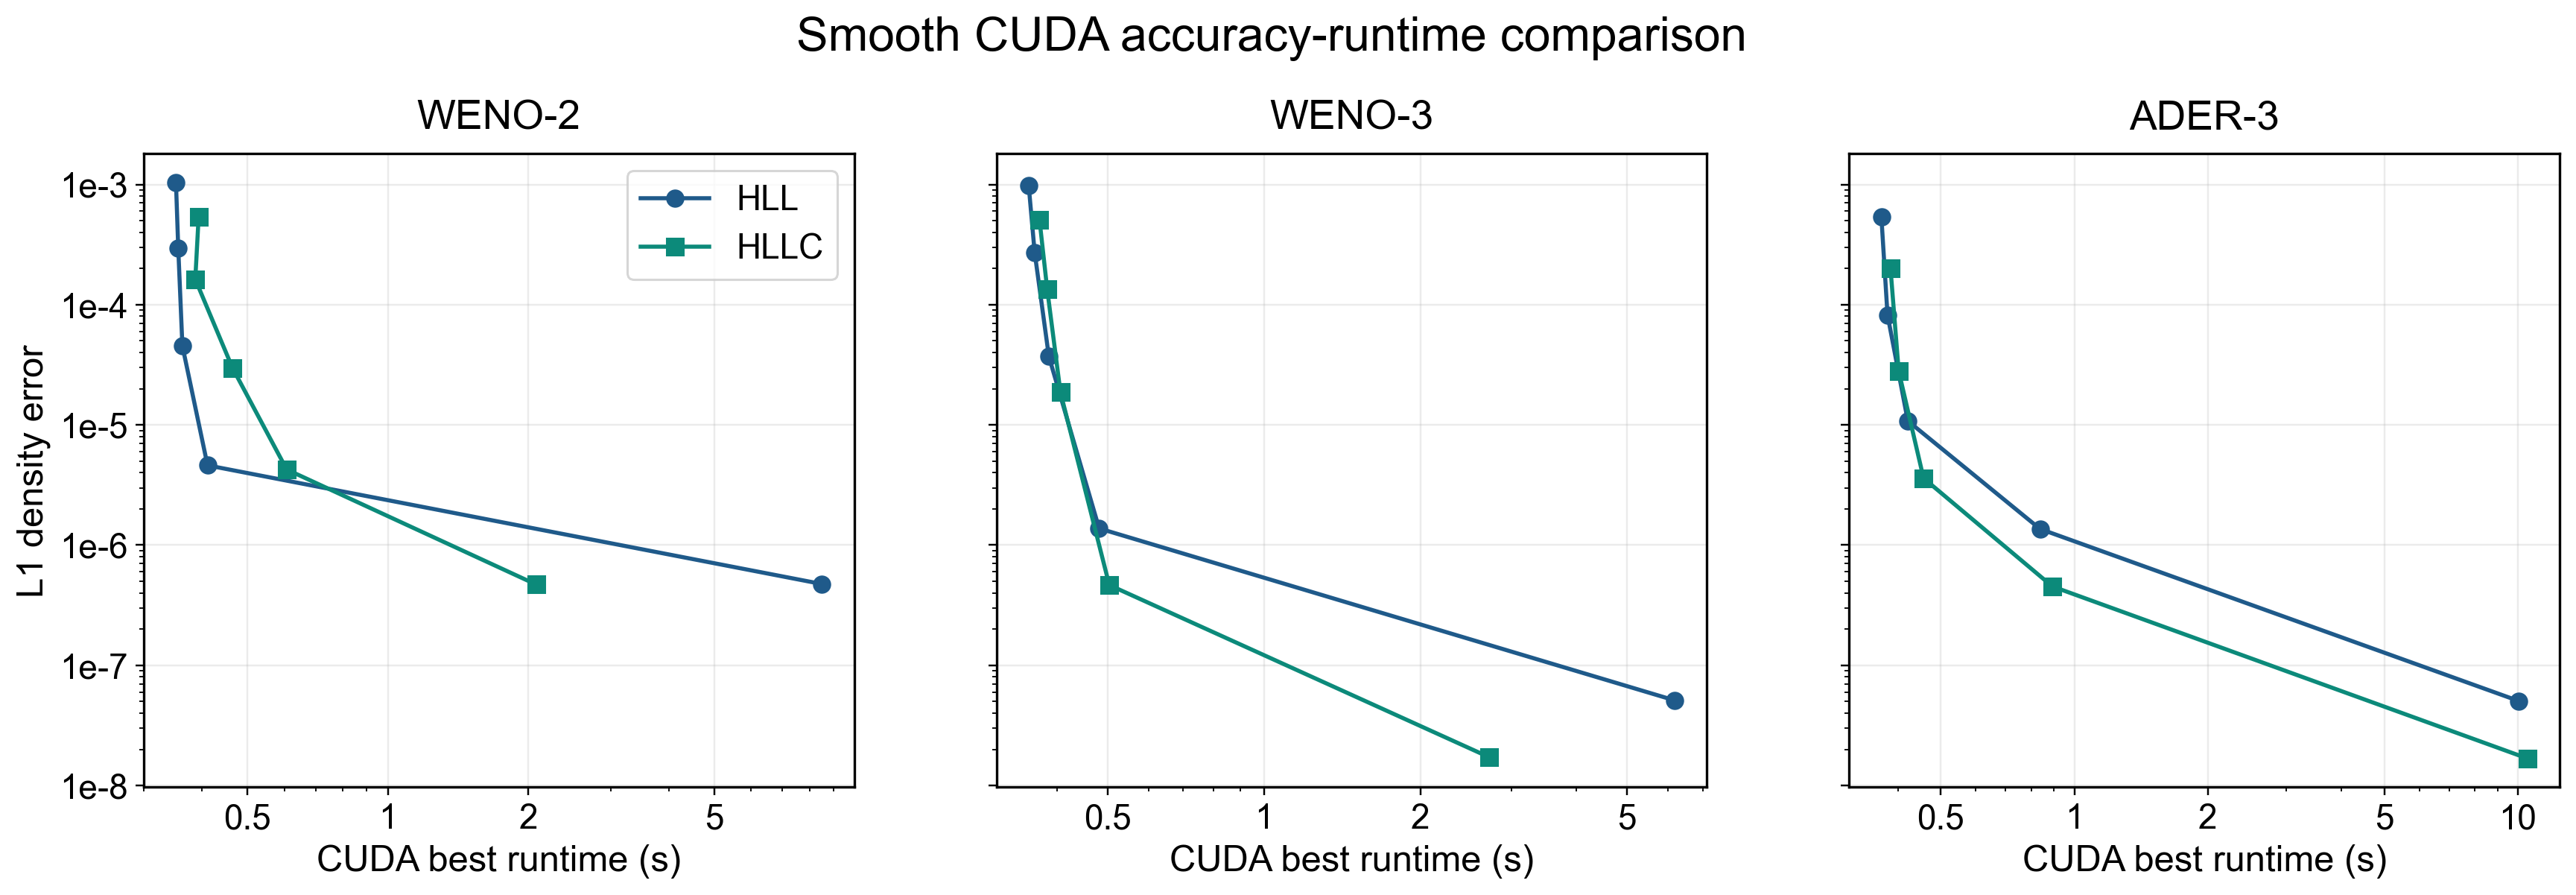
\includegraphics[width=0.92\textwidth]{performance_hll_hllc_cuda_tradeoff.png}
\caption{Matched smooth CUDA accuracy--runtime trajectories for HLL and HLLC across the
common grid sequence.}
\label{fig:hll-hllc-cuda-tradeoff}
\end{figure}

Figure~\ref{fig:hll-hllc-cuda-tradeoff} confirms that the \(600^2\) result is not an
isolated endpoint.  For WENO-3 and ADER-3, the HLLC curve remains below the HLL curve over
the refinement sequence, so it reaches a lower density error for a comparable cost.  The
HLL evidence therefore strengthens rather than displaces the HLLC conclusion: HLLC is the
appropriate authoritative dataset, while HLL provides a useful performance baseline.

\section{Phase-resolved acceleration and bottlenecks}

End-to-end speedup identifies the best backend but does not explain why it wins.  A separate
instrumented campaign therefore accumulated time in five groups:
\begin{itemize}[leftmargin=1.8em]
  \item setup/workspace/transfer: initialization, temporary flux arrays, and explicit
        host--device transfer timing.
  \item CFL reduction: characteristic-speed evaluation and the global maximum reduction.
  \item spatial operator: reconstruction or local prediction, HLLC interface fluxes, and
        assembly of the spatial residual.
  \item update/validity: conservative state update, admissibility checks, and retry logic.
  \item other: profiled time not assigned to the preceding categories.
\end{itemize}
The profiler was run at \(100^2\), where fixed costs are visible, and \(600^2\), where
the stencil work dominates.  Three repeats were used at \(100^2\). The \(600^2\) profiles
are single diagnostic runs.

\begin{figure}[H]
\centering
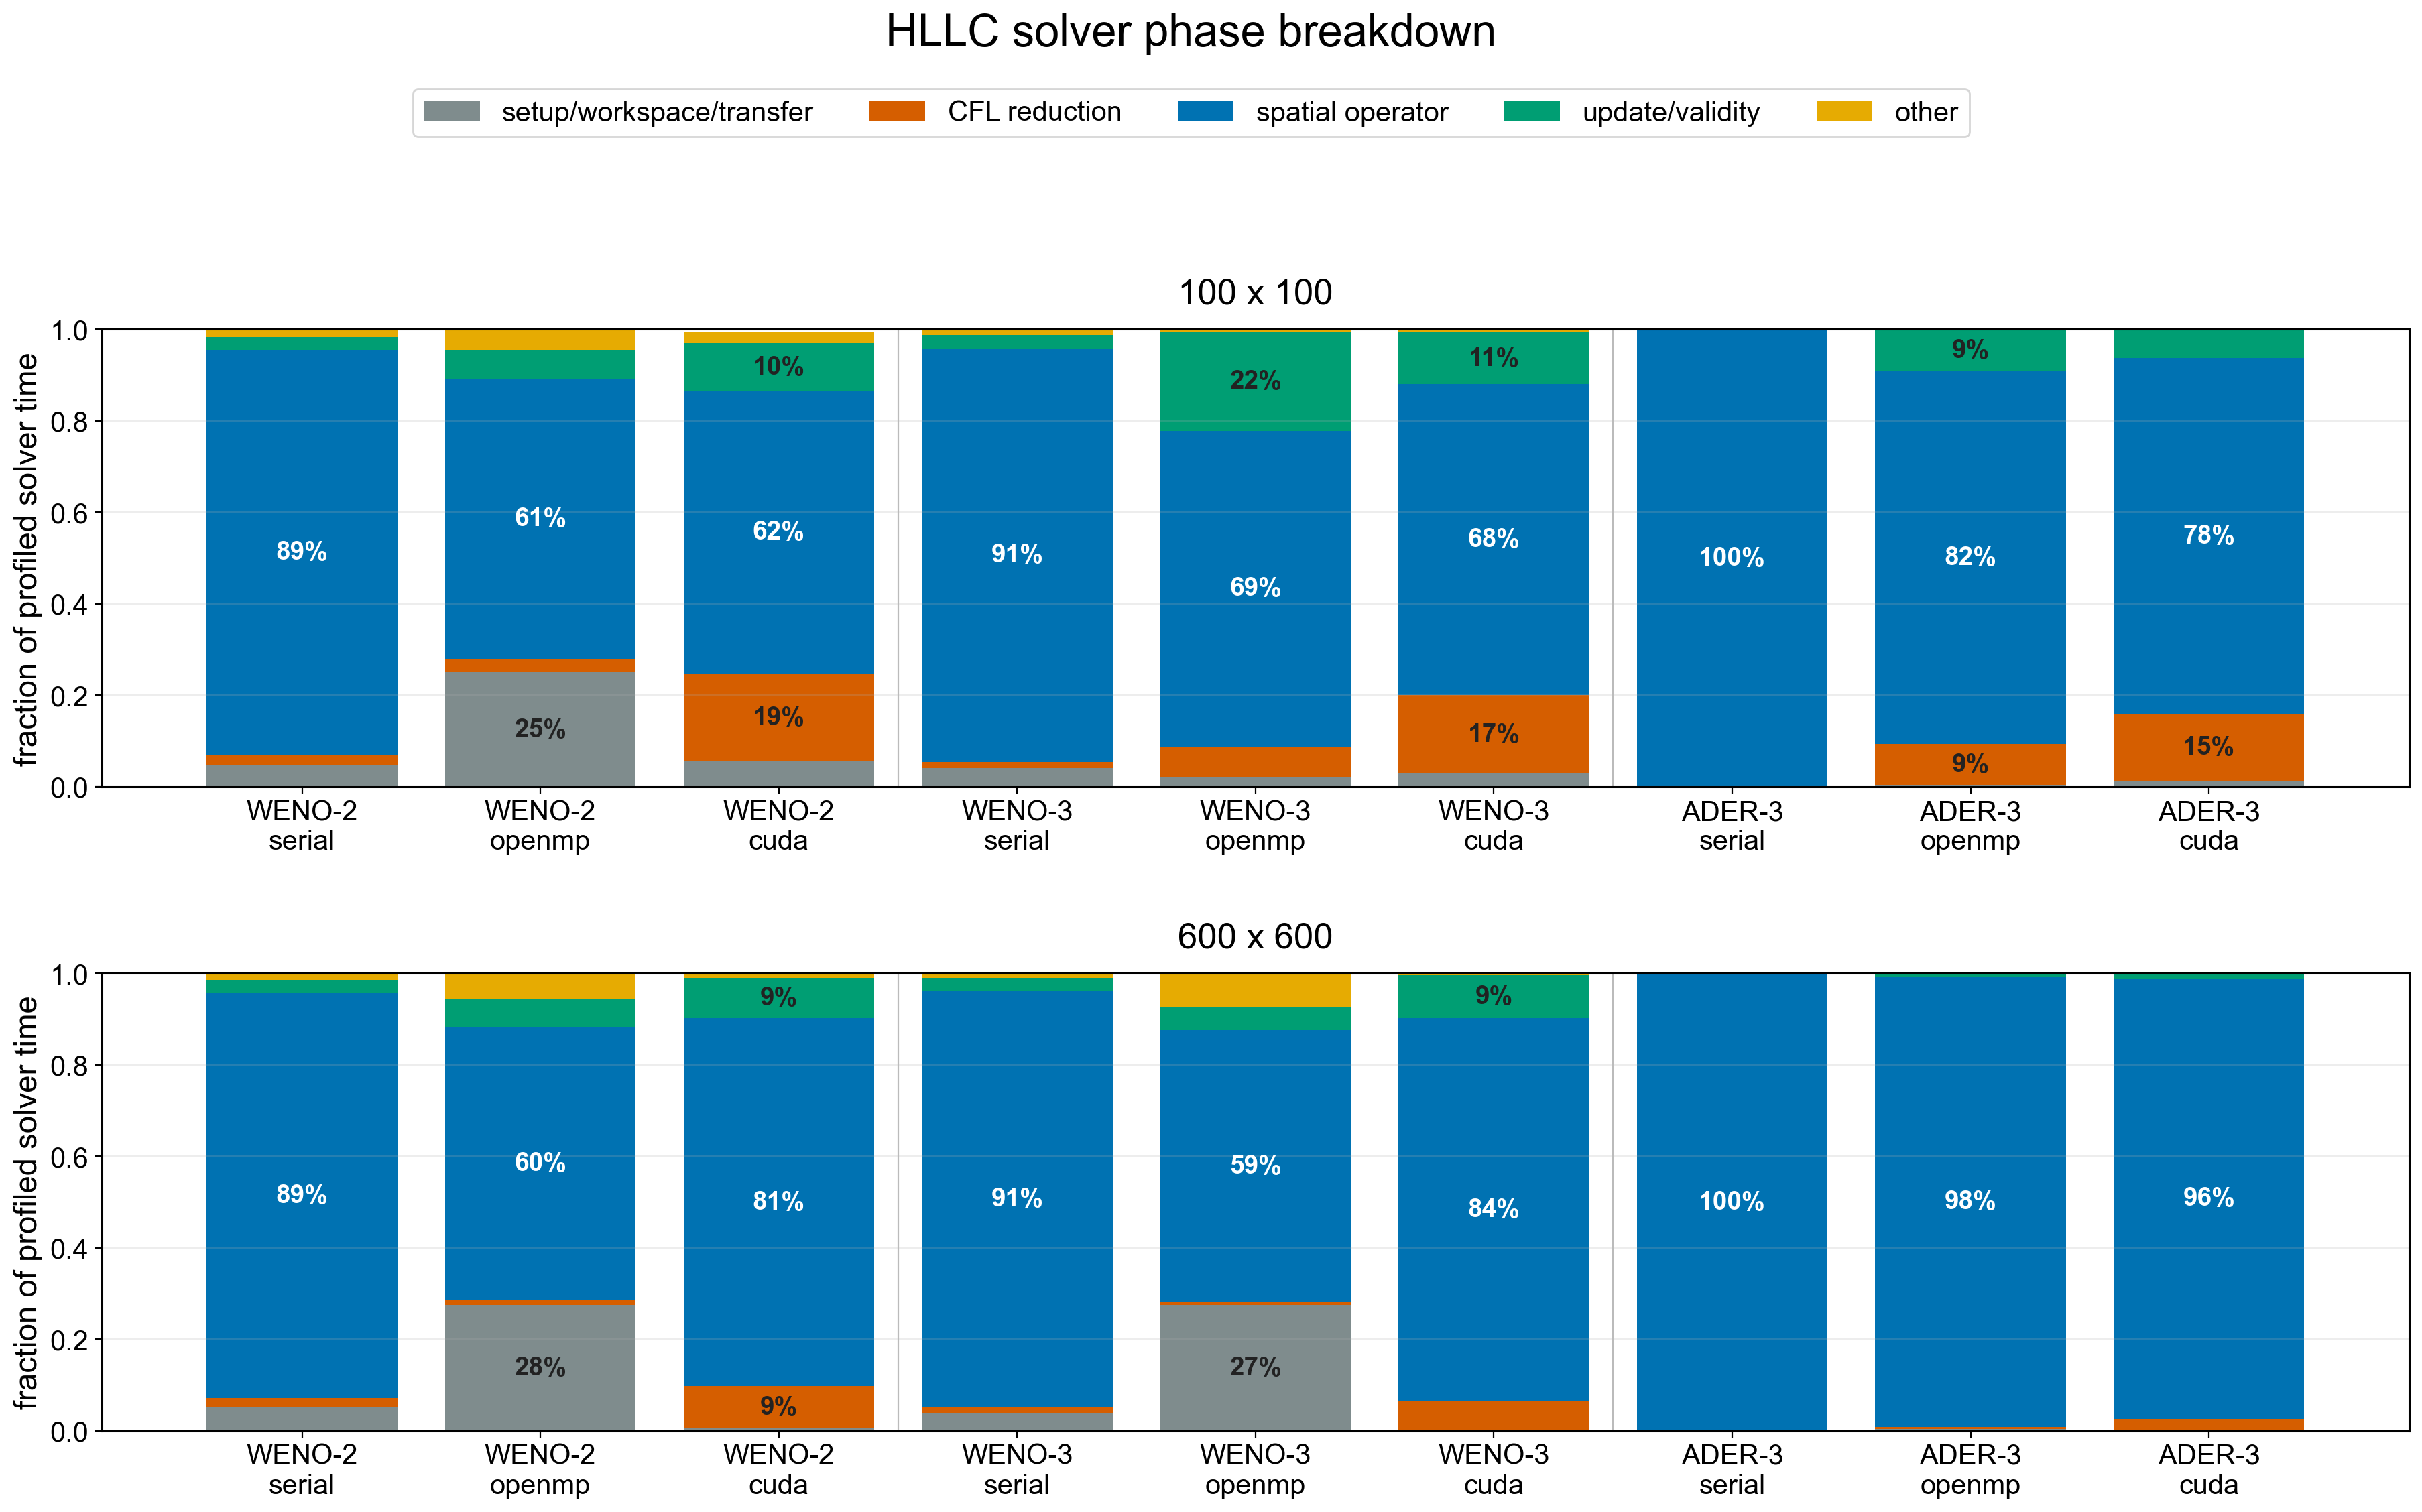
\includegraphics[width=0.98\textwidth]{performance_phase_breakdown_hllc.png}
\caption{Fraction of instrumented HLLC solver time assigned to each phase at
\(100\times100\) and \(600\times600\).}
\label{fig:phase-breakdown-performance}
\end{figure}

The spatial operator is the principal cost in every large-grid run.  Its serial share is
88.6\% for WENO-2, 91.0\% for WENO-3, and 99.7\% for ADER-3.  On OpenMP, the WENO share
falls to about 59.5\% because workspace management and the less scalable update phases
become visible after the main loops are accelerated.  ADER-3 remains 98.4\% spatial on
OpenMP because its local predictor is so expensive that fixed overhead is comparatively
small.  On CUDA, the spatial shares are 80.5\%, 83.8\%, and 96.3\%. The residual CFL and
state-update phases account for most of the remaining time.

\begin{table}[H]
\centering
\small
\begin{tabular}{lrrr|rr}
\toprule
& \multicolumn{3}{c|}{Spatial share (\%)} & \multicolumn{2}{c}{Spatial speedup} \\
Method & Serial & OpenMP & CUDA & OpenMP & CUDA \\
\midrule
WENO-2 & 88.6 & 59.5 & 80.5 & 12.20 & 204.06 \\
WENO-3 & 91.0 & 59.5 & 83.8 & 10.52 & 205.64 \\
ADER-3 & 99.7 & 98.4 & 96.3 & 11.36 & 1049.00 \\
\bottomrule
\end{tabular}
\caption{Spatial-operator share and comparable phase speedup at \(600\times600\).
Phase speedups are relative to the instrumented serial phase for the same method.}
\label{tab:phase-spatial}
\end{table}

\begin{figure}[H]
\centering
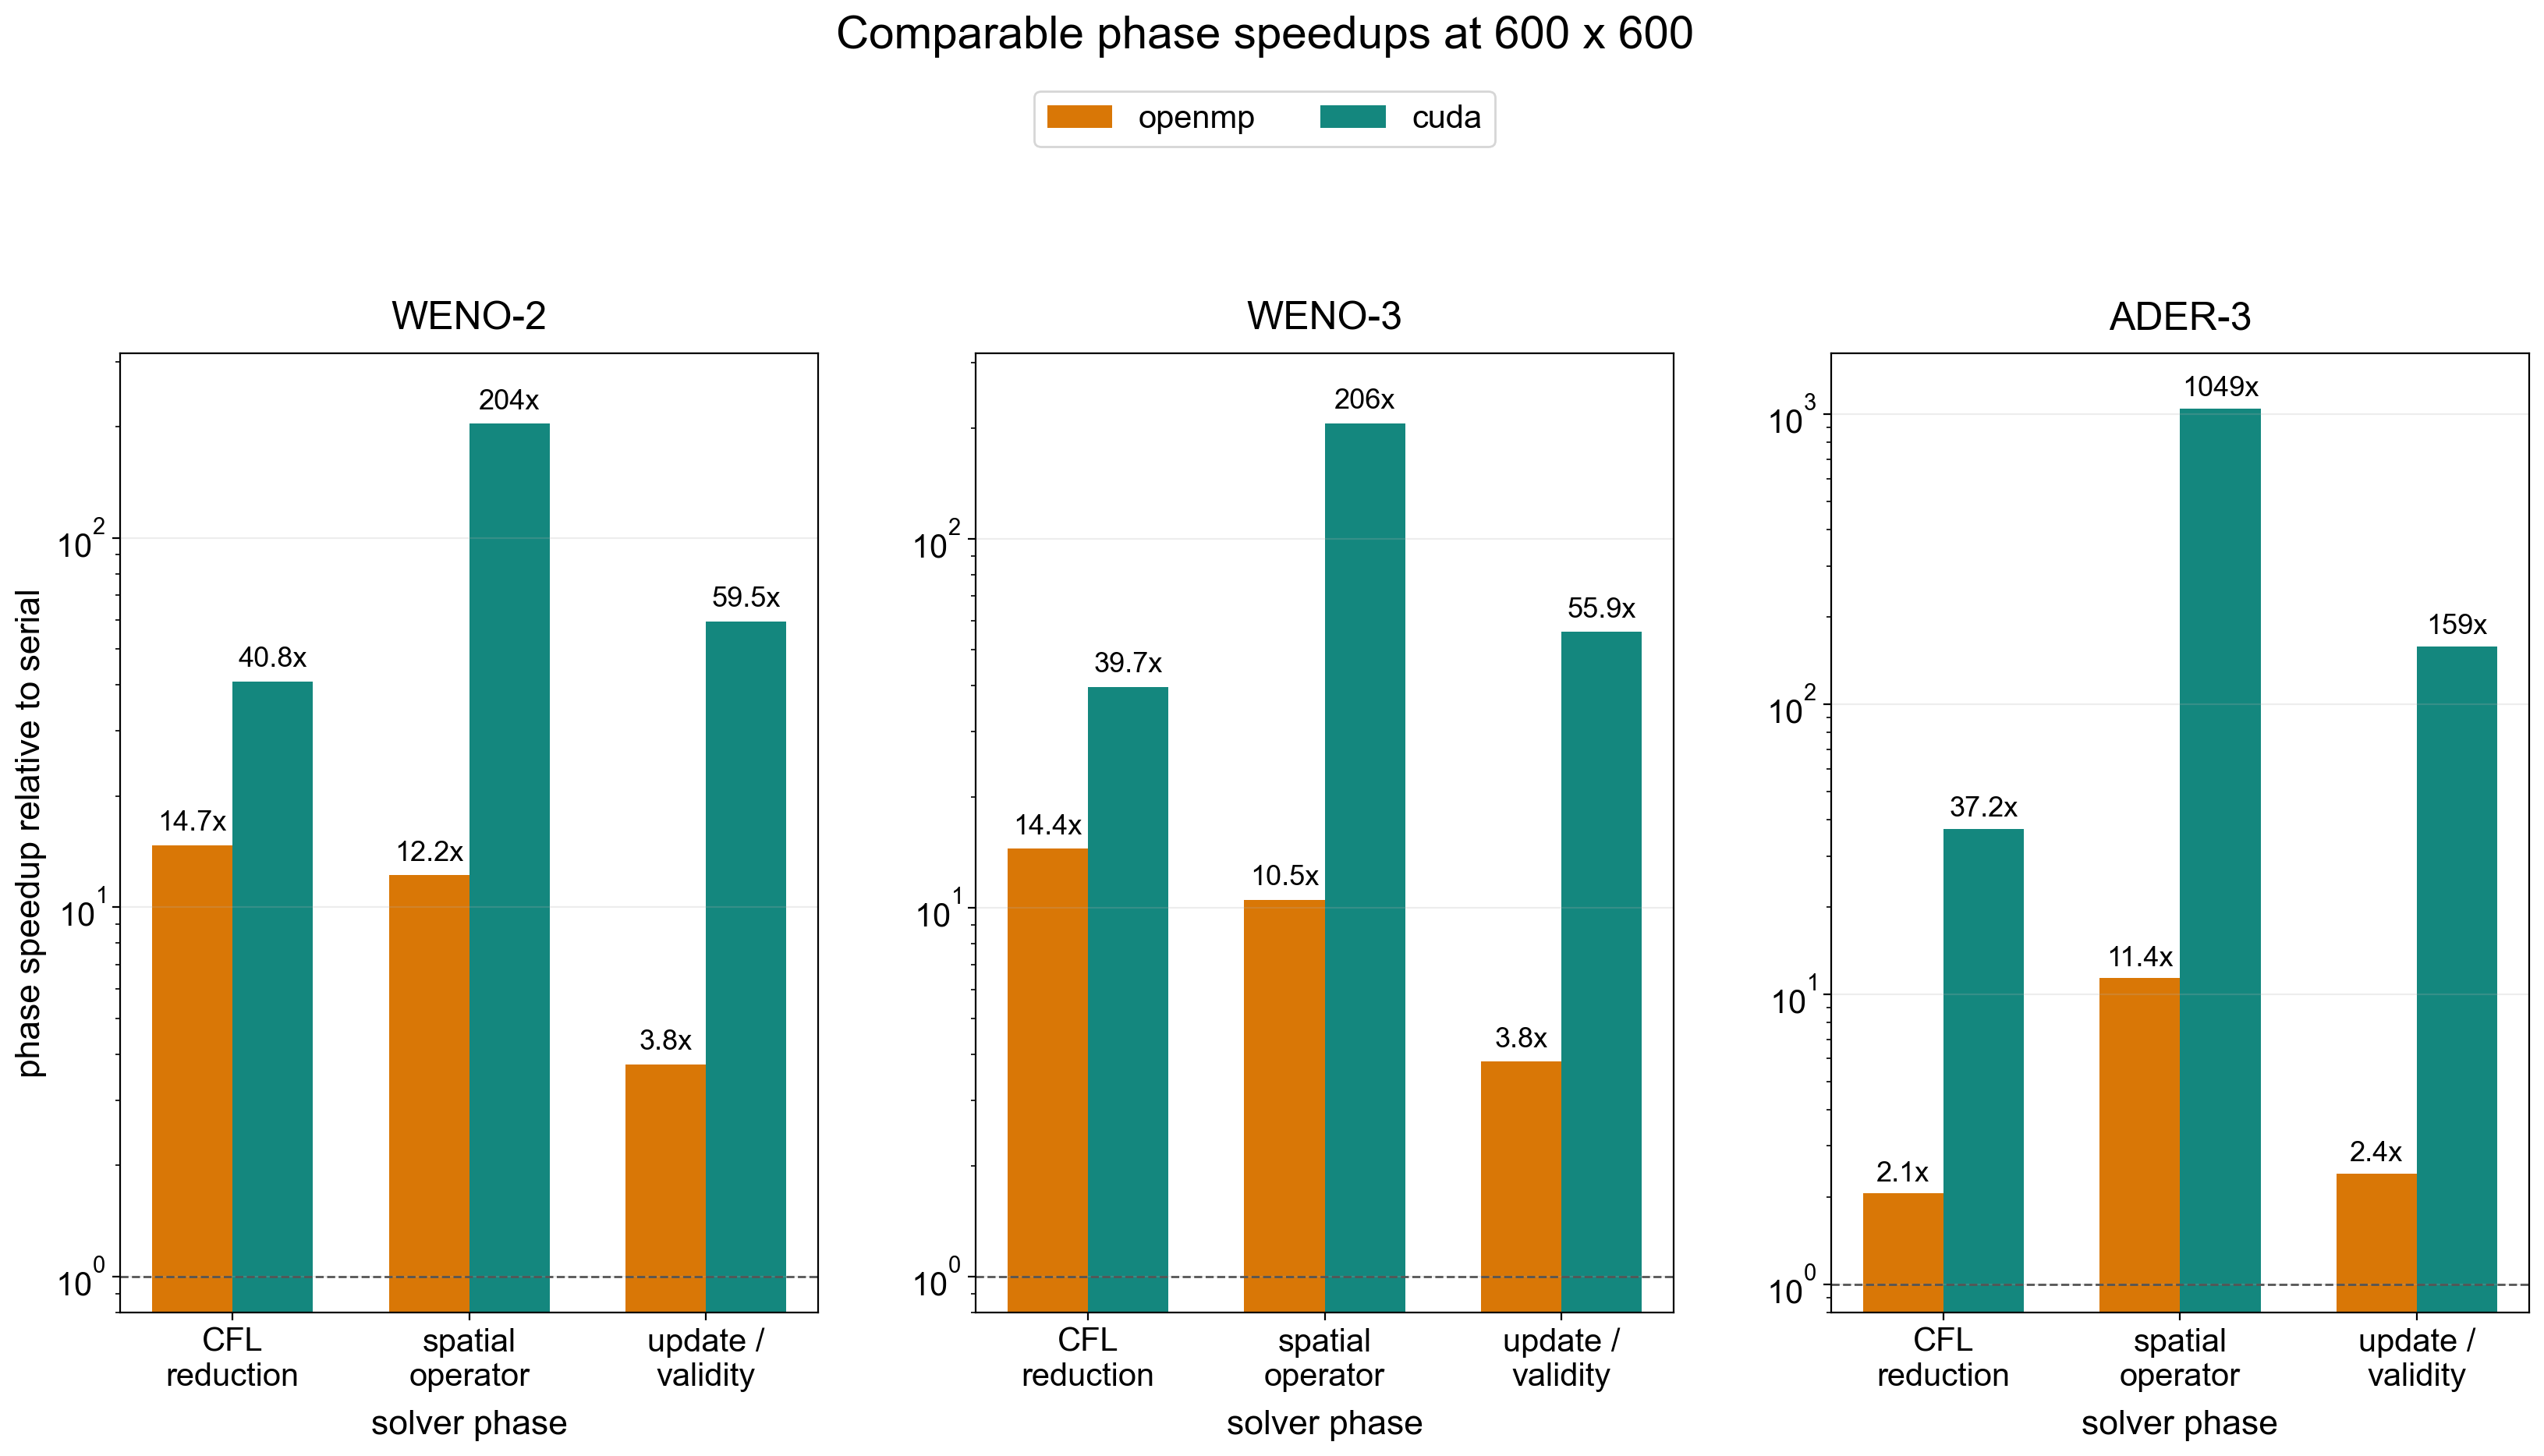
\includegraphics[width=0.98\textwidth]{performance_phase_speedup_hllc.png}
\caption{Comparable HLLC phase speedups at \(600\times600\).  The aggregate
setup/workspace/transfer category is omitted because its CPU and CUDA implementation
boundaries are not identical.}
\label{fig:phase-speedup-performance}
\end{figure}

Figure~\ref{fig:phase-speedup-performance} gives the clearest optimization priorities.
CUDA reduces the WENO spatial operators by about 204--206 times and the ADER-3 spatial
operator by roughly 1049 times.  Once that dominant work is accelerated, CFL reduction and
the final update become the limiting fractions. This is the expected Amdahl-type shift
\cite{amdahl1967}.
For OpenMP, the spatial loops still accelerate by approximately 10.5--12.2 times, but
end-to-end WENO speedup is reduced by workspace allocation, synchronization, and update
work.  ADER-3 has an additional OpenMP bottleneck: its CFL and update phases accelerate by
only about 2.05 and 2.41, respectively, even though the predictor-dominated spatial phase
scales well.

The phase measurements are diagnostic, not replacements for the canonical timings in
Table~\ref{tab:smooth-n600-performance}.  CUDA phase boundaries require explicit
synchronization to obtain meaningful kernel times, and those synchronizations change the
measured total.  The profiler is therefore used to assign cost and identify bottlenecks.
All headline runtime and speedup claims continue to use the ordinary no-output campaign.

\section{OpenMP thread scaling}

The thread experiment isolates CPU scaling on the smooth \(100^2\) case using the OpenMP
shared-memory model \cite{openmp52} and \(p=1,2,4,8,16\).
Table~\ref{tab:openmp-thread-scaling} and
Figure~\ref{fig:openmp-thread-scaling-performance} show that method complexity determines
how long additional threads remain useful.  WENO-2 reaches only 4.20 times speedup at 16
threads, equivalent to 26.3\% parallel efficiency. WENO-3 reaches 5.33 and 33.3\%.
ADER-3 reaches 14.30 and 89.4\%, because its compute-heavy predictor supplies enough
independent work to dominate thread launch, synchronization, and memory-management costs.
The bounded efficiencies are consistent with Amdahl's observation that non-parallel work
limits total speedup even when the dominant loop scales well \cite{amdahl1967}.

\begin{table}[H]
\centering
\begin{tabular}{lrrrr}
\toprule
Method & \(T_1\) (s) & \(T_{16}\) (s) & \(S_{16}\) & \(E_{16}\) \\
\midrule
WENO-2 & 0.4483 & 0.1066 & 4.20 & 26.3\% \\
WENO-3 & 1.0475 & 0.1966 & 5.33 & 33.3\% \\
ADER-3 & 19.1913 & 1.3422 & 14.30 & 89.4\% \\
\bottomrule
\end{tabular}
\caption{HLLC OpenMP scaling from one to 16 threads at \(100\times100\).}
\label{tab:openmp-thread-scaling}
\end{table}

\begin{figure}[H]
\centering
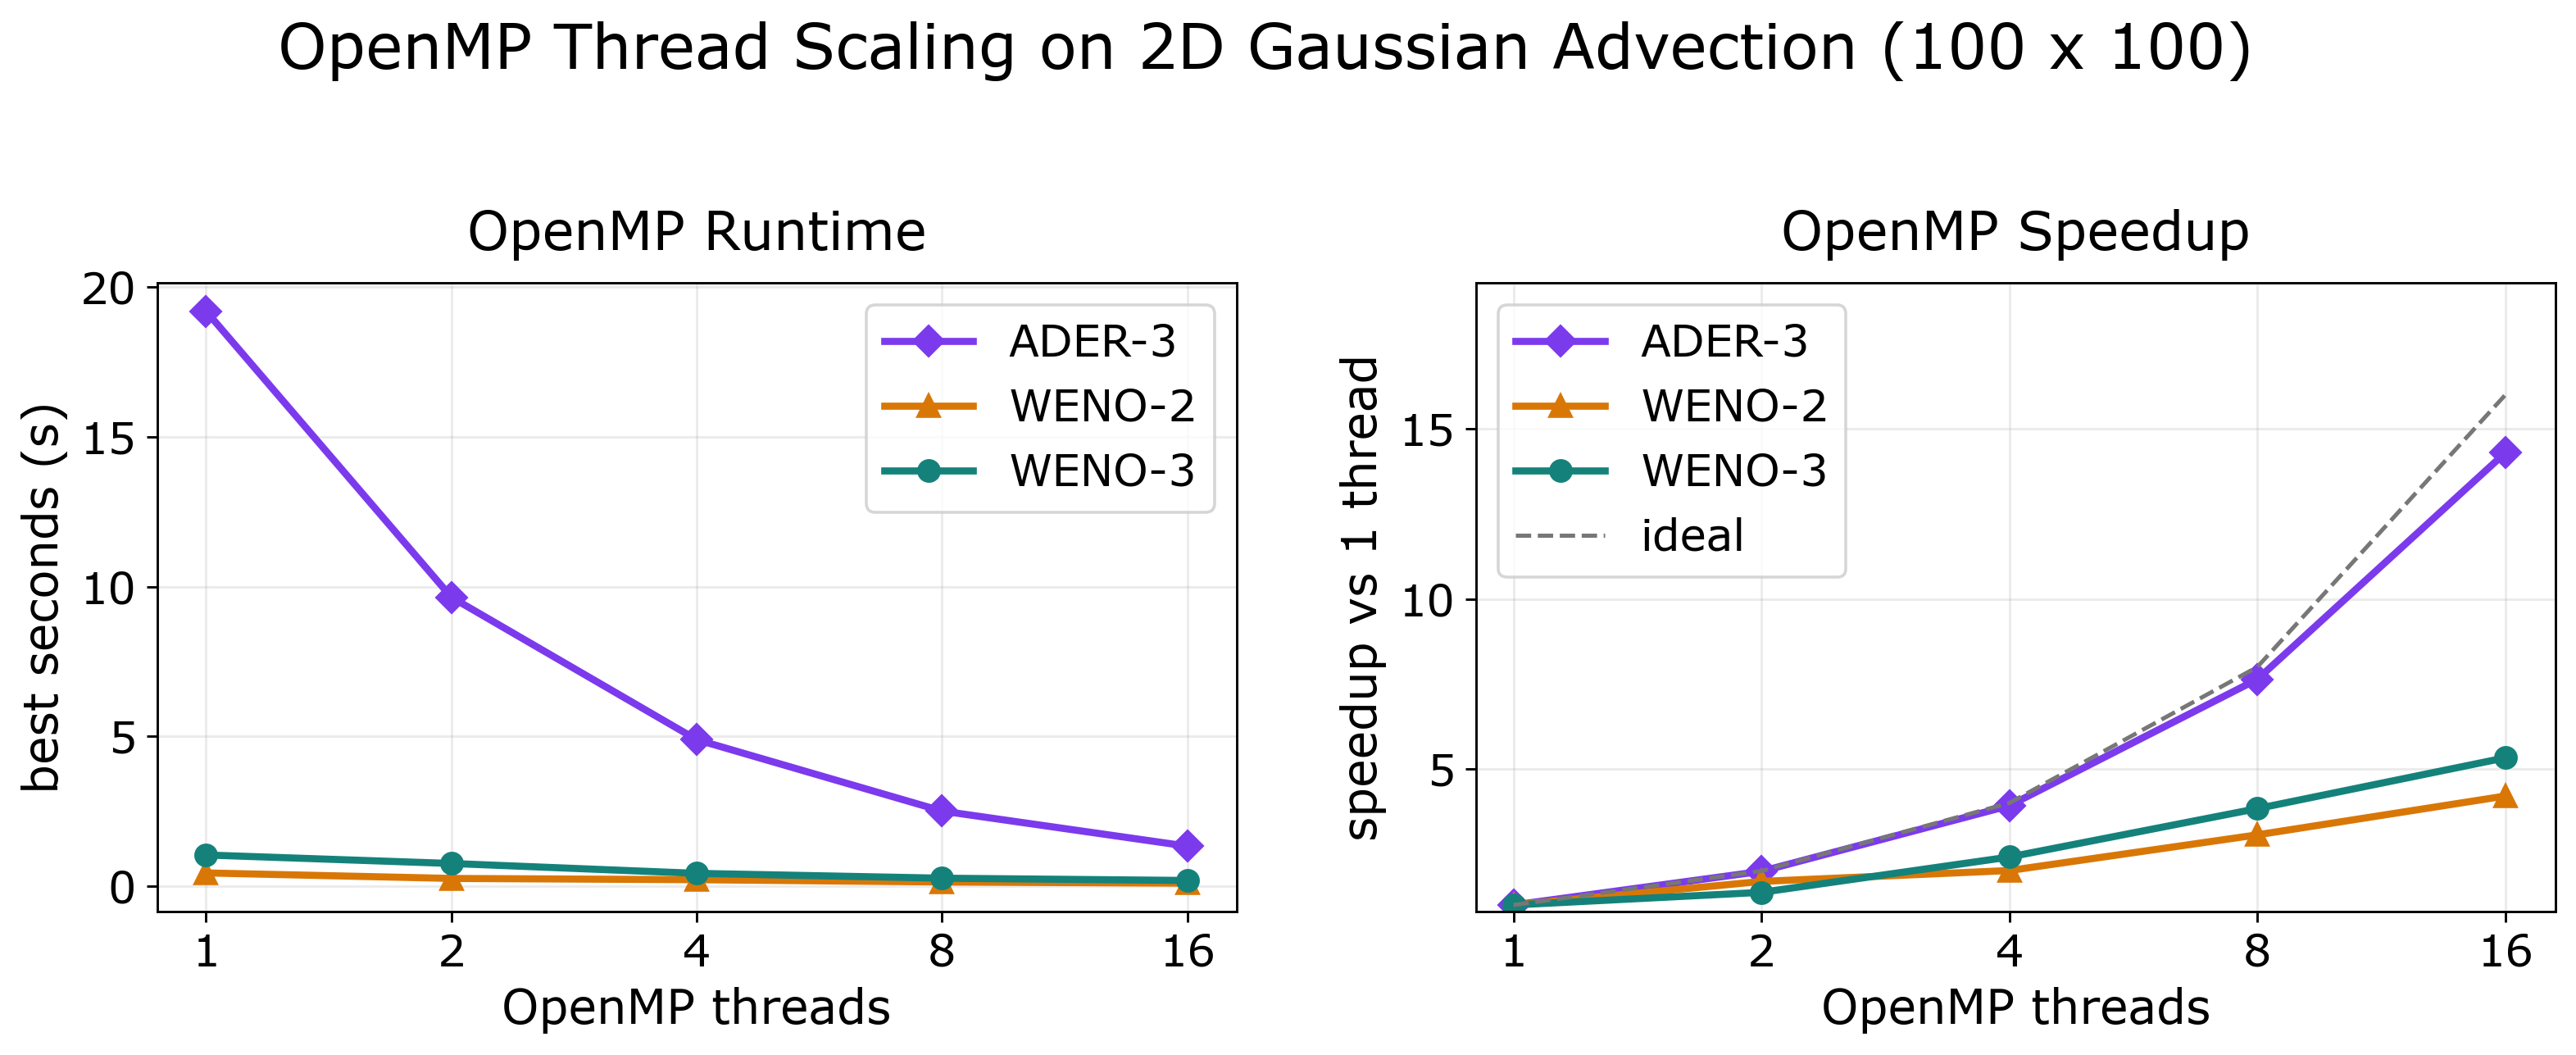
\includegraphics[width=0.88\textwidth]{performance_openmp_threads_hllc.png}
\caption{HLLC OpenMP runtime and speedup at \(100\times100\).  The corresponding
16-thread parallel efficiencies are listed in Table~\ref{tab:openmp-thread-scaling}.}
\label{fig:openmp-thread-scaling-performance}
\end{figure}

The early saturation of WENO-2 is therefore not evidence that its numerical method has
failed. It is a workload-granularity result.  A cheaper stencil leaves a larger fraction of
the run in work that is fixed, memory-bound, or repeatedly synchronized.  ADER-3 is the
opposite case: it is expensive in absolute terms, but that expense is highly parallel.

\section{CUDA scaling envelope}

The all-backend campaign stops at \(600^2\) because serial ADER-3 is already very slow.
A CUDA-only sweep extends the smooth calculation to ten resolutions between \(n=600\)
and \(n=5000\).  The sampled sequence is
\(600, 1000, 1400, 1800, 2400\), followed by
\(3000, 3600, 4200, 4600,\) and \(5000\).  In a two-dimensional explicit scheme the
number of cells scales as \(n^2\), while the CFL condition makes the number of time steps
approximately proportional to \(n\).  A well-behaved large-grid runtime is therefore
expected to approach
\begin{equation}
  T(n)\propto n^3.
  \label{eq:cubic-work}
\end{equation}
Here \(n\) is the number of cells in each coordinate direction and \(T(n)\) is
the measured CUDA runtime on the resulting \(n\times n\) grid.
The local empirical exponent between adjacent points is
\begin{equation}
  p_{12}=\frac{\log(T_2/T_1)}{\log(n_2/n_1)}.
  \label{eq:local-runtime-exponent}
\end{equation}
The subscripts 1 and 2 identify two consecutive grid sizes:
\(T_1=T(n_1)\) and \(T_2=T(n_2)\). Therefore \(p_{12}\approx3\) is consistent
with the expected cubic work growth, while a substantially larger value marks
a locally steeper runtime increase. It is a scaling diagnostic, not a formal
accuracy order.

\begin{figure}[H]
\centering
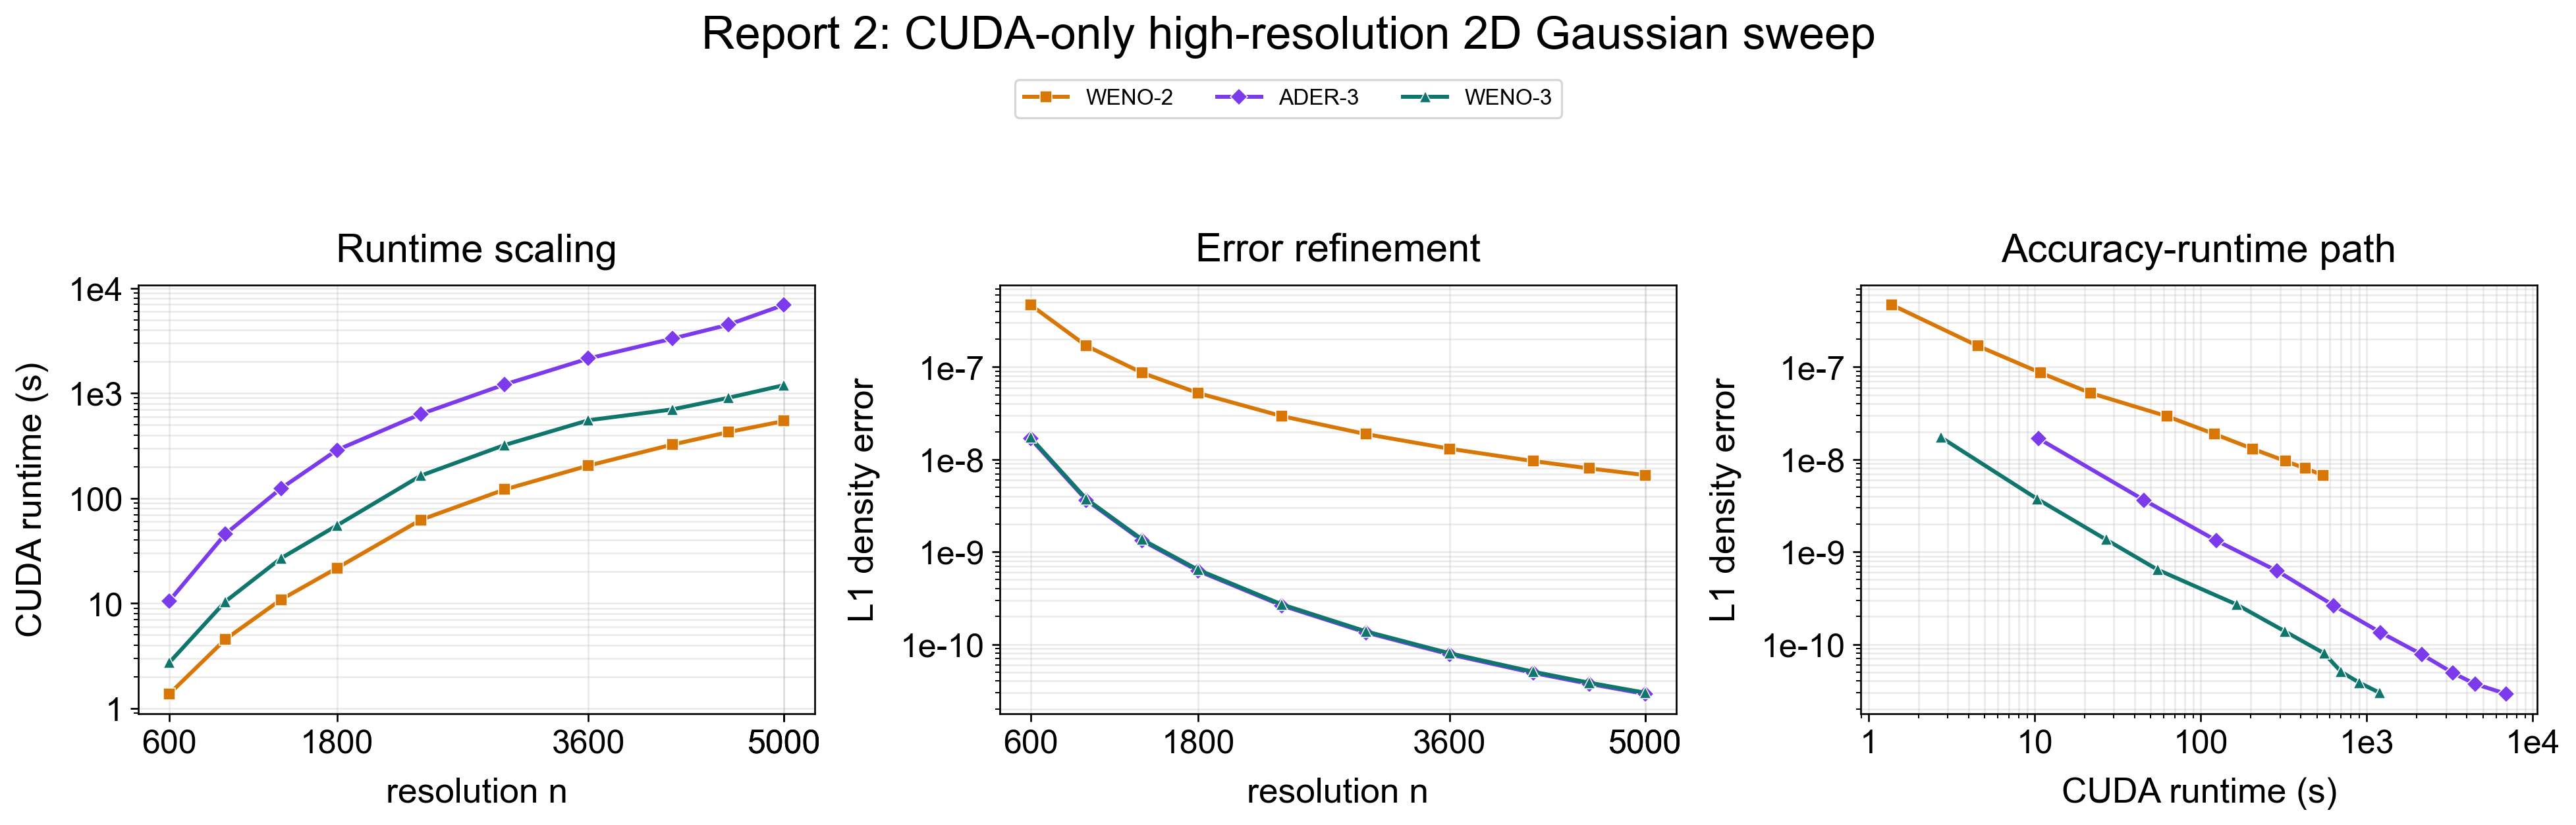
\includegraphics[width=0.98\textwidth]{performance_gpu_limit_hllc.png}
\caption{HLLC CUDA-only large-grid runtime, density error, and accuracy--runtime
trade-off through the official \(5000\times5000\) endpoint.}
\label{fig:gpu-envelope-performance}
\end{figure}

\begin{table}[H]
\centering
\begin{tabular}{lrrr}
\toprule
Method & \(T(5000)\) (s) & \(L_1(\rho)\) & Final \(p_{12}\) \\
\midrule
WENO-2 & 543.78 & \(6.769\times10^{-9}\) & 2.92 \\
WENO-3 & 1193.21 & \(2.996\times10^{-11}\) & 3.34 \\
ADER-3 & 6935.73 & \(2.908\times10^{-11}\) & 5.24 \\
\bottomrule
\end{tabular}
\caption{Largest official HLLC CUDA point and final-interval runtime exponent.  The final
exponent is a one-repeat diagnostic and is not treated as a precise hardware limit.}
\label{tab:gpu-limit-endpoint}
\end{table}

Across the complete \(600\)--\(5000\) sweep, the resolution increases by a factor of
\(8.333\), so ideal cubic work would increase by \(8.333^3=578.7\).  The measured runtime
factors are \(395.5\), \(436.9\), and \(657.2\) for WENO-2, WENO-3, and ADER-3,
respectively.  Equation~\eqref{eq:local-runtime-exponent} applied to the two endpoints
therefore gives overall exponents of \(2.82\), \(2.87\), and \(3.06\).  WENO-2 and WENO-3
grow slightly less rapidly than the nominal work count because the larger grids amortise
fixed launch and setup costs more effectively. ADER-3 is almost exactly cubic over the
full range despite its steeper final segment.

The error reduction is equally diagnostic.  From \(600^2\) to \(5000^2\),
\(L_1(\rho)\) falls by factors of \(69.5\), \(576.1\), and \(578.2\).  These values closely
match the theoretical refinement factors \(8.333^2=69.4\) for WENO-2 and
\(8.333^3=578.7\) for the two third-order methods.  Thus the large-grid sweep is not merely
making the calculation more expensive: it continues to deliver the expected second- and
third-order error reductions throughout the measured range.

The endpoint comparison quantifies the accuracy--cost trade-off.  At \(5000^2\), WENO-3
is \(2.19\) times slower than WENO-2 but reduces the density error by a factor of
\(225.9\).  ADER-3 is \(12.75\) times slower than WENO-2 and reduces the error by a similar
factor of \(232.8\).  Comparing only the third-order routes, ADER-3 costs \(5.81\) times as
much as WENO-3 for a further error reduction of only \(2.97\) percent.  WENO-3 is therefore
the stronger accuracy--efficiency choice at the largest accepted grid, even though ADER-3
attains the smallest absolute \(L_1(\rho)\).

The final two local runtime exponents are \(3.00\) and \(2.92\) for WENO-2,
\(2.79\) and \(3.34\) for WENO-3, and \(3.35\) and \(5.24\) for ADER-3.  The first two
methods consequently remain close to cubic scaling at the end of the sweep.  ADER-3's
\(4600\)--\(5000\) increase is substantially steeper and is consistent with growing memory
pressure or reduced kernel efficiency, but this final exponent comes from one repeat at
each endpoint and cannot by itself identify a unique hardware cause.

\section{Performance synthesis}

The measurements lead to a consistent hardware-dependent ranking.  WENO-2 is the cheapest
method when moderate accuracy or very small grids are sufficient.  WENO-3 gives a large
error reduction at modest CUDA cost and is the best overall accuracy--efficiency compromise
in the current implementation.  ADER-3 achieves the expected third-order accuracy and the
largest parallel speedups, but its local predictor makes it expensive in absolute time.

OpenMP is useful for all three methods, particularly ADER-3, but its scaling is bounded by
workspace, synchronization, CFL reduction, and update work.  CUDA is the decisive backend
once the grid is large enough. Phase profiling shows that it accelerates precisely the
reconstruction, prediction, and flux work that dominates the solvers.  HLLC also improves
the third-order smooth errors relative to the matched HLL baseline without imposing a
consistent runtime penalty.  These results justify using HLLC and WENO-3 as the main
accuracy--efficiency route, while retaining ADER-3 as an informative high-order one-step
comparison and WENO-2 as the Report~1 reference.

\FloatBarrier

\chapter{Integrated discussion}
\label{chap:discussion}

The experiments separate three questions that are often conflated in method comparisons:
whether the designed order is recovered, whether different implementations solve the same
discrete problem, and whether the resulting accuracy is obtained at a useful cost.  The
combined evidence now permits a direct answer.  Higher order is valuable in this code, but
only when the reconstruction or predictor is paired with hardware that can amortise its
additional work.  Among the tested combinations, WENO-3 with HLLC on CUDA gives the most
consistent balance of accuracy, robustness, and runtime.

\section{When does higher order justify its cost?}

On smooth advection, WENO-3 and ADER-3 recover third order while WENO-2 recovers second
order.  This formal distinction remains visible in the practical \(600^2\) experiment:
WENO-3 and ADER-3 reduce \(L_1(\rho)\) by factors of 27.2 and 28.0 relative to WENO-2.
The two third-order errors are almost identical, so runtime decides between them.  On CUDA,
WENO-3 costs 2.71 s compared with 2.08 s for WENO-2, whereas ADER-3 costs 10.51 s.
WENO-3 therefore purchases most of the available smooth-case accuracy improvement for a
small additional GPU cost.  ADER-3 verifies that the one-step construction is accurate and
highly parallel, but its present predictor does not improve the error enough to recover its
larger absolute cost.

The discontinuous evidence changes the criterion.  Formal order is no longer achieved at
shocks, so contact resolution, positivity, and local oscillation become more important
than the smooth convergence slope.  WENO-3 again gives the strongest compromise: it is
less diffusive than WENO-2 around narrow structures, remains close to WENO-2 in the
far-field states, and costs substantially less than ADER-3.  The ADER-3 fallback prevents
catastrophic failure and preserves positive states, but the predictor/fallback transition
introduces the largest local backend sensitivity and does not give a uniformly cleaner
field.  Thus the main advantage of ADER-3 in the current code is its demonstration of a
robust, one-step third-order route rather than superiority on every test.

\section{What changes when HLL is replaced by HLLC?}

HLLC is the authoritative flux because the tested Euler problems contain material contacts
that are absent from the two-wave HLL model.  The matched comparison in
Figure~\ref{fig:hll-hllc-n600-tradeoff} also shows that this decision is supported by the
computed data rather than by theory alone.  At \(600^2\), changing from HLL to HLLC alters
the WENO-2 density error by less than 1\%, but lowers the WENO-3 and ADER-3 errors by about
66\%.  A more accurate reconstruction can therefore expose the benefit of the contact wave
more clearly than the second-order reference.

The runtime comparison is deliberately interpreted as implementation evidence.  HLLC is
not algebraically cheaper than HLL, yet the stored WENO HLLC paths are faster because the
complete kernels differ in branching, memory traffic, and compiler output.  ADER-3, for
which the predictor dominates the flux cost, changes by only 4.8\% on CUDA.  The defensible
conclusion is consequently that HLLC improves the measured accuracy and is not prohibitively
expensive in this implementation. It is not that HLLC must always run faster than HLL.

\section{Suitability of each backend}

Serial execution remains essential as the transparent reference implementation, but its
cost rises rapidly for the third-order methods.  OpenMP is most useful in an intermediate
regime.  It avoids CUDA's fixed launch and device-management costs on small grids and gives
useful speedup on a shared-memory CPU, but its efficiency eventually flattens.  The phase
profile explains why: once the stencil loops are parallel, workspace allocation, reductions,
updates, barriers, and memory bandwidth occupy a larger fraction of the run.  At 16 threads
and \(100^2\), the measured efficiencies are 26.3\%, 33.3\%, and 89.4\% for WENO-2,
WENO-3, and ADER-3.  The compute-heavy ADER predictor supplies enough work to use the
threads effectively, whereas the lighter WENO loops encounter overhead sooner.

CUDA is the appropriate backend for large grids and for the two third-order methods.  At
\(600^2\), smooth speedups reach 38.43 for WENO-2, 83.84 for WENO-3, and 392.01 for
ADER-3.  Phase profiling attributes this gain to the spatial operator: its CUDA speedup is
about 204 for both WENO methods and 1049 for ADER-3.  Acceleration therefore shifts the
bottleneck rather than removing it.  CFL reduction and state update become visible once the
dominant stencil or predictor work has been shortened.  Future optimization should target
those residual phases and reduce synchronization, rather than only tuning an already fast
flux kernel.

\begin{table}[H]
\centering
\small
\renewcommand{\arraystretch}{1.30}
\begin{tabular}{p{0.25\textwidth}p{0.26\textwidth}p{0.40\textwidth}}
\toprule
Objective & Recommended route & Reason \tabularnewline
\midrule
Low-cost reference or modest accuracy & WENO-2 on serial/OpenMP & Lowest method cost, useful before CUDA overhead is amortised. \tabularnewline
High smooth accuracy & WENO-3/HLLC on CUDA & Near-third-order error at a runtime close to CUDA WENO-2. \tabularnewline
Contact-rich discontinuous flow & WENO-3/HLLC on CUDA & Better local resolution than WENO-2 without ADER-3's present cost and sensor sensitivity. \tabularnewline
One-step high-order research route & ADER-3/HLLC on CUDA & Correct smooth order and very large parallel speedup, but further predictor/fallback optimization is required. \tabularnewline
\bottomrule
\end{tabular}
\caption{Recommended method/backend combinations within the tested problem range.}
\label{tab:recommendations}
\end{table}

\section{Limits of the evidence}

The conclusions are bounded by the experiment design.  The Gaussian problem supplies an
exact error measure, but the two-dimensional discontinuous cases do not. Their assessment
therefore combines positivity, backend agreement, field structure, and one-dimensional
slices.  Timings are best repeated values on a shared node and are intended to suppress
transient interference, not to reproduce an exclusively reserved machine.  The phase
profiler inserts CUDA synchronizations to assign kernel time and is diagnostic rather than
the source of the headline runtimes.

The official large-grid study ends at \(5000^2\).  It shows continued accuracy reduction
and increasing CUDA cost, but no single sharp saturation point that can be defended from
runtime slope alone.  Larger exploratory points were more sensitive to memory pressure and
shared-machine variability and were therefore not promoted into the canonical results.
Finally, the ADER-3 troubled-interface decision is intentionally nonlinear.  Small backend
roundoff can change a branch near its threshold, so a localized difference larger than
roundoff is possible even when both solutions remain conservative, positive, and physically
equivalent at the resolved scale.

\chapter{Conclusions and future work}
\label{chap:conclusions}

Report~2 asked whether third-order finite-volume methods provide enough additional accuracy
to justify their cost on serial, OpenMP, and CUDA hardware.  The answer is conditional but
clear.  Both WENO-3/SSPRK3 and ADER-3 recover third order on smooth one- and two-dimensional
advection, while WENO-2 provides the expected second-order reference.  HLLC preserves the
contact wave and, in the matched smooth comparison, reduces the WENO-3 and ADER-3 density
errors by about two thirds relative to the older HLL route.  Serial, OpenMP, and CUDA fields
agree to roundoff or to small localized differences associated with nonlinear fallback
decisions, and every accepted high-resolution discontinuous field retains positive density
and pressure.

The decisive result is the interaction between method and backend.  On the smooth
\(600^2\) problem, CUDA WENO-3 achieves \(L_1(\rho)=1.726\times10^{-8}\) in 2.71 s,
compared with \(4.703\times10^{-7}\) in 2.08 s for WENO-2.  ADER-3 gives a similar error,
\(1.681\times10^{-8}\), but requires 10.51 s.  WENO-3/HLLC on CUDA is therefore the best
overall accuracy--efficiency combination tested.  WENO-2 remains the appropriate economical
baseline, especially for small grids.  ADER-3 is numerically successful and exposes much
greater parallelism than either WENO route, but the present local predictor and robust
fallback make it too expensive to be the default choice.

The discontinuous cases reinforce rather than overturn this ranking.  WENO-3 retains
contacts more sharply than WENO-2 at a manageable CUDA cost.  ADER-3 captures the same wave
pattern and remains admissible, but its local sensor transitions are more visible and its
absolute runtime is highest.  Higher formal order is therefore not sufficient by itself:
the useful method is the one whose robustness mechanism, flux, and hardware implementation
preserve the accuracy benefit at an acceptable cost.

The phase-resolved measurements identify concrete next steps.  First, OpenMP work arrays
should be allocated once and reused, and adjacent loops should be fused where this reduces
barriers and memory traffic.  Second, CUDA CFL reduction, conservative update, and validity
checks should be fused or reorganised to reduce the residual synchronization exposed after
the spatial operator is accelerated.  Third, the ADER predictor and troubled-interface
criterion should be profiled together. A smoother or characteristic-based sensor may reduce
branch sensitivity without sacrificing positivity.  Characteristic-variable WENO and a
more selective fallback are also natural numerical extensions.

Further performance work should use reserved or otherwise controlled GPU measurements,
hardware counters, and a profiler such as Nsight to separate cache, bandwidth, occupancy,
and allocation effects.  Adaptive mesh refinement would then be a more informative route
to larger effective resolution than uniform grids beyond \(5000^2\).  A longer project
could additionally examine multi-GPU decomposition and vary the shock--bubble size to test
how active-region geometry affects thread occupancy and load balance.

The principal outcome is consequently not a universal winner independent of context.
It is a tested selection rule: use WENO-2 when low cost is primary, use WENO-3/HLLC on CUDA
when accuracy and robustness must both be retained, and treat ADER-3 as a promising one-step
route whose numerical machinery is ready but whose implementation still offers substantial
scope for optimization.

\begin{thebibliography}{99}

\bibitem{harten1983}
A. Harten, P. D. Lax, and B. van Leer,
On upstream differencing and Godunov-type schemes for hyperbolic conservation laws,
\emph{SIAM Review} 25 (1983), 35--61.
\href{https://doi.org/10.1137/1025002}{doi:10.1137/1025002}.

\bibitem{toro1994}
E. F. Toro, M. Spruce, and W. Speares,
Restoration of the contact surface in the HLL-Riemann solver,
\emph{Shock Waves} 4 (1994), 25--34.
\href{https://doi.org/10.1007/BF01414629}{doi:10.1007/BF01414629}.

\bibitem{toro2009}
E. F. Toro,
\emph{Riemann Solvers and Numerical Methods for Fluid Dynamics},
3rd ed., Springer, 2009.
\href{https://doi.org/10.1007/b79761}{doi:10.1007/b79761}.

\bibitem{henrick2005}
A. K. Henrick, T. D. Aslam, and J. M. Powers,
Mapped weighted essentially non-oscillatory schemes: achieving optimal order near critical points,
\emph{Journal of Computational Physics} 207 (2005), 542--567.
\href{https://doi.org/10.1016/j.jcp.2005.01.023}{doi:10.1016/j.jcp.2005.01.023}.

\bibitem{jiang1996}
G.-S. Jiang and C.-W. Shu,
Efficient implementation of weighted ENO schemes,
\emph{Journal of Computational Physics} 126 (1996), 202--228.
\href{https://doi.org/10.1006/jcph.1996.0130}{doi:10.1006/jcph.1996.0130}.

\bibitem{borges2008}
R. Borges, M. Carmona, B. Costa, and W. S. Don,
An improved weighted essentially non-oscillatory scheme for hyperbolic conservation laws,
\emph{Journal of Computational Physics} 227 (2008), 3191--3211.
\href{https://doi.org/10.1016/j.jcp.2007.11.038}{doi:10.1016/j.jcp.2007.11.038}.

\bibitem{gottlieb2001}
S. Gottlieb, C.-W. Shu, and E. Tadmor,
Strong stability-preserving high-order time discretization methods,
\emph{SIAM Review} 43 (2001), 89--112.
\href{https://doi.org/10.1137/S003614450036757X}{doi:10.1137/S003614450036757X}.

\bibitem{dumbser2008}
M. Dumbser, C. Enaux, and E. F. Toro,
Finite volume schemes of very high order of accuracy for stiff hyperbolic balance laws,
\emph{Journal of Computational Physics} 227 (2008), 3971--4001.
\href{https://doi.org/10.1016/j.jcp.2007.12.005}{doi:10.1016/j.jcp.2007.12.005}.

\bibitem{courant1967}
R. Courant, K. Friedrichs, and H. Lewy,
On the partial difference equations of mathematical physics,
\emph{IBM Journal of Research and Development} 11 (1967), 215--234.
\href{https://doi.org/10.1147/rd.112.0215}{doi:10.1147/rd.112.0215}.

\bibitem{amdahl1967}
G. M. Amdahl,
Validity of the single processor approach to achieving large scale computing capabilities,
in \emph{Proceedings of the AFIPS Spring Joint Computer Conference}, 1967, pp.~483--485.
\href{https://doi.org/10.1145/1465482.1465560}{doi:10.1145/1465482.1465560}.

\bibitem{williams2009}
S. Williams, A. Waterman, and D. Patterson,
Roofline: an insightful visual performance model for multicore architectures,
\emph{Communications of the ACM} 52 (2009), 65--76.
\href{https://doi.org/10.1145/1498765.1498785}{doi:10.1145/1498765.1498785}.

\bibitem{openmp52}
OpenMP Architecture Review Board,
\emph{OpenMP Application Programming Interface, Version 5.2}, November 2021.
\href{https://www.openmp.org/spec-html/5.2/openmp.html}{openmp.org/spec-html/5.2}.

\bibitem{nvidia129}
NVIDIA Corporation,
\emph{CUDA C++ Programming Guide, CUDA Toolkit 12.9}, 2025.
\href{https://docs.nvidia.com/cuda/archive/12.9.0/cuda-c-programming-guide/contents.html}{docs.nvidia.com/cuda/archive/12.9.0}.

\end{thebibliography}


\end{document}
